%----------------------------------------------------------------------------------------
%	PACKAGES AND OTHER DOCUMENT CONFIGURATIONS
%----------------------------------------------------------------------------------------

\documentclass[
11pt,
oneside,
english,
singlespacing,
%liststotoc, % Uncomment to add the list of figures/tables/etc to the table of contents
%toctotoc, % Uncomment to add the main table of contents to the table of contents
%nohyperref, % Uncomment to not load the hyperref package
headsepline,
%consistentlayout, % Uncomment to change the layout of the declaration, abstract and acknowledgements pages to match the default layout
]{MastersDoctoralThesis}

\usepackage[utf8]{inputenc}
\usepackage[T1]{fontenc} % Output font encoding for international characters
\usepackage{markdown}
\usepackage{palatino}

\usepackage[backend=biber,style=authoryear,natbib=true]{biblatex} % Use the bibtex backend with the authoryear citation style (which resembles APA)

\addbibresource{bibliography.bib}

\usepackage[autostyle=true]{csquotes} % Required to generate language-dependent quotes in the bibliography

\usepackage{float}

\usepackage{pdfpages}

\usepackage{hyperref}

% ------------------------------------------------ Including code in doc
\usepackage{listings}
\usepackage{color}

\definecolor{dkgreen}{rgb}{0,0.6,0}
\definecolor{gray}{rgb}{0.5,0.5,0.5}
\definecolor{mauve}{rgb}{0.58,0,0.82}
\lstset{frame=tb,
  language=Python,
  aboveskip=3mm,
  belowskip=3mm,
  showstringspaces=false,
  columns=flexible,
  basicstyle={\small\ttfamily},
  numbers=none,
  numberstyle=\tiny\color{gray},
  keywordstyle=\color{blue},
  commentstyle=\color{dkgreen},
  stringstyle=\color{mauve},
  breaklines=true,
  breakatwhitespace=true,
  tabsize=3
}

%----------------------------------------------------------------------------------------
%	MARGIN SETTINGS
%----------------------------------------------------------------------------------------

\usepackage{amsmath}

%----------------------------------------------------------------------------------------
%	MARGIN SETTINGS
%----------------------------------------------------------------------------------------

\geometry{
	paper=a4paper,
	inner=2.5cm,
	outer=3.8cm,
	bindingoffset=.5cm,
	top=1.5cm,
	bottom=1.5cm,
}

%----------------------------------------------------------------------------------------
%	THESIS INFORMATION
%----------------------------------------------------------------------------------------

\thesistitle{Collaborative Genre Tagging} %\ttitle
\supervisor{Dr Miguel \textsc{Lacerda}} %\supname
\examiner{} %\examname
\degree{M.Sc. Data Science} %\degreename
\author{James \textsc{Leslie}} %\authorname
\addresses{} %\addressname

\subject{Data Science} %\subjectname
\keywords{} %\keywordnames
\university{\href{https://www.uct.ac.za/}{University Of Cape Town}} %\univname
\department{\href{http://www.science.uct.ac.za/sci/departments/study-statistical-sciences}{Department of Statistical Sciences}} %\deptname
\group{\href{http://www.science.uct.ac.za/}{Faculty of Science}} %\groupname
\faculty{\href{http://www.ebe.uct.ac.za/}{Faculty of Science}} %\facname

% \AtBeginDocument{
% \hypersetup{pdftitle=\ttitle} % Set the PDF's title to your title
% \hypersetup{pdfauthor=\authorname} % Set the PDF's author to your name
% \hypersetup{pdfkeywords=\keywordnames} % Set the PDF's keywords to your keywords
% }

\begin{document}

\frontmatter % Use roman page numbering style (i, ii, iii, iv...) for the pre-content pages

\pagestyle{plain} % Default to the plain heading style until the thesis style is called for the body content

%----------------------------------------------------------------------------------------
%	TITLE PAGE
%----------------------------------------------------------------------------------------

\begin{titlepage}
\begin{center}

\vspace*{.06\textheight}
{\scshape\LARGE \univname\par}\vspace{1.5cm} % University name
\textsc{\Large Research Project}\\[0.5cm] % Thesis type

\HRule \\[0.4cm] % Horizontal line
{\huge \bfseries \ttitle\par}\vspace{0.4cm} % Thesis title
\HRule \\[1.5cm] % Horizontal line
 
\begin{minipage}[t]{0.4\textwidth}
\begin{flushleft} \large
\emph{Author:}\\
\href{https://james-leslie.github.io/E-Portfolio/}{\authorname} % Author name - remove the \href bracket to remove the link
\end{flushleft}
\end{minipage}
\begin{minipage}[t]{0.4\textwidth}
\begin{flushright} \large
\emph{Supervisor:} \\
\href{http://www.geomatics.uct.ac.za/geomatics/staff/george-sithole}{\supname} % Supervisor name - remove the \href bracket to remove the link  
\end{flushright}
\end{minipage}\\[3cm]
 
\vfill

\large \textit{A project submitted in fulfilment of the requirements\\ for the degree of \degreename}\\[0.3cm]
\textit{in the}\\[0.4cm]
\groupname\\\deptname\\[2cm]
\vfill

{\large \today}\\[4cm] % Date
%\includegraphics{Logo} % University/department logo - uncomment to place it
 
\vfill
\end{center}
\end{titlepage}

%----------------------------------------------------------------------------------------
%	DECLARATION PAGE
%----------------------------------------------------------------------------------------

\begin{declaration}
\addchaptertocentry{\authorshipname} % Add the declaration to the table of contents
\noindent I, \authorname, declare that this project titled, \enquote{\ttitle} and the work presented in it are my own. I confirm that:

\begin{itemize} 
\item This work was done wholly or mainly while in candidature for a master's degree at this University.
\item Where any part of this dissertation has previously been submitted for a degree or any other qualification at this University or any other institution, this has been clearly stated.
\item Where I have consulted the published work of others, this is always clearly attributed.
\item Where I have quoted from the work of others, the source is always given. With the exception of such quotations, this project is entirely my own work.
\item I have acknowledged all main sources of help.
\item Where the project is based on work done by myself jointly with others, I have made clear exactly what was done by others and what I have contributed myself.
\end{itemize}
\vspace{5em}
\noindent Signed:\\
\rule[0.5em]{25em}{0.5pt} % This prints a line for the signature
 
\noindent Date:\\
\rule[0.5em]{25em}{0.5pt} % This prints a line to write the date
\end{declaration}

\cleardoublepage

% include PDF
% 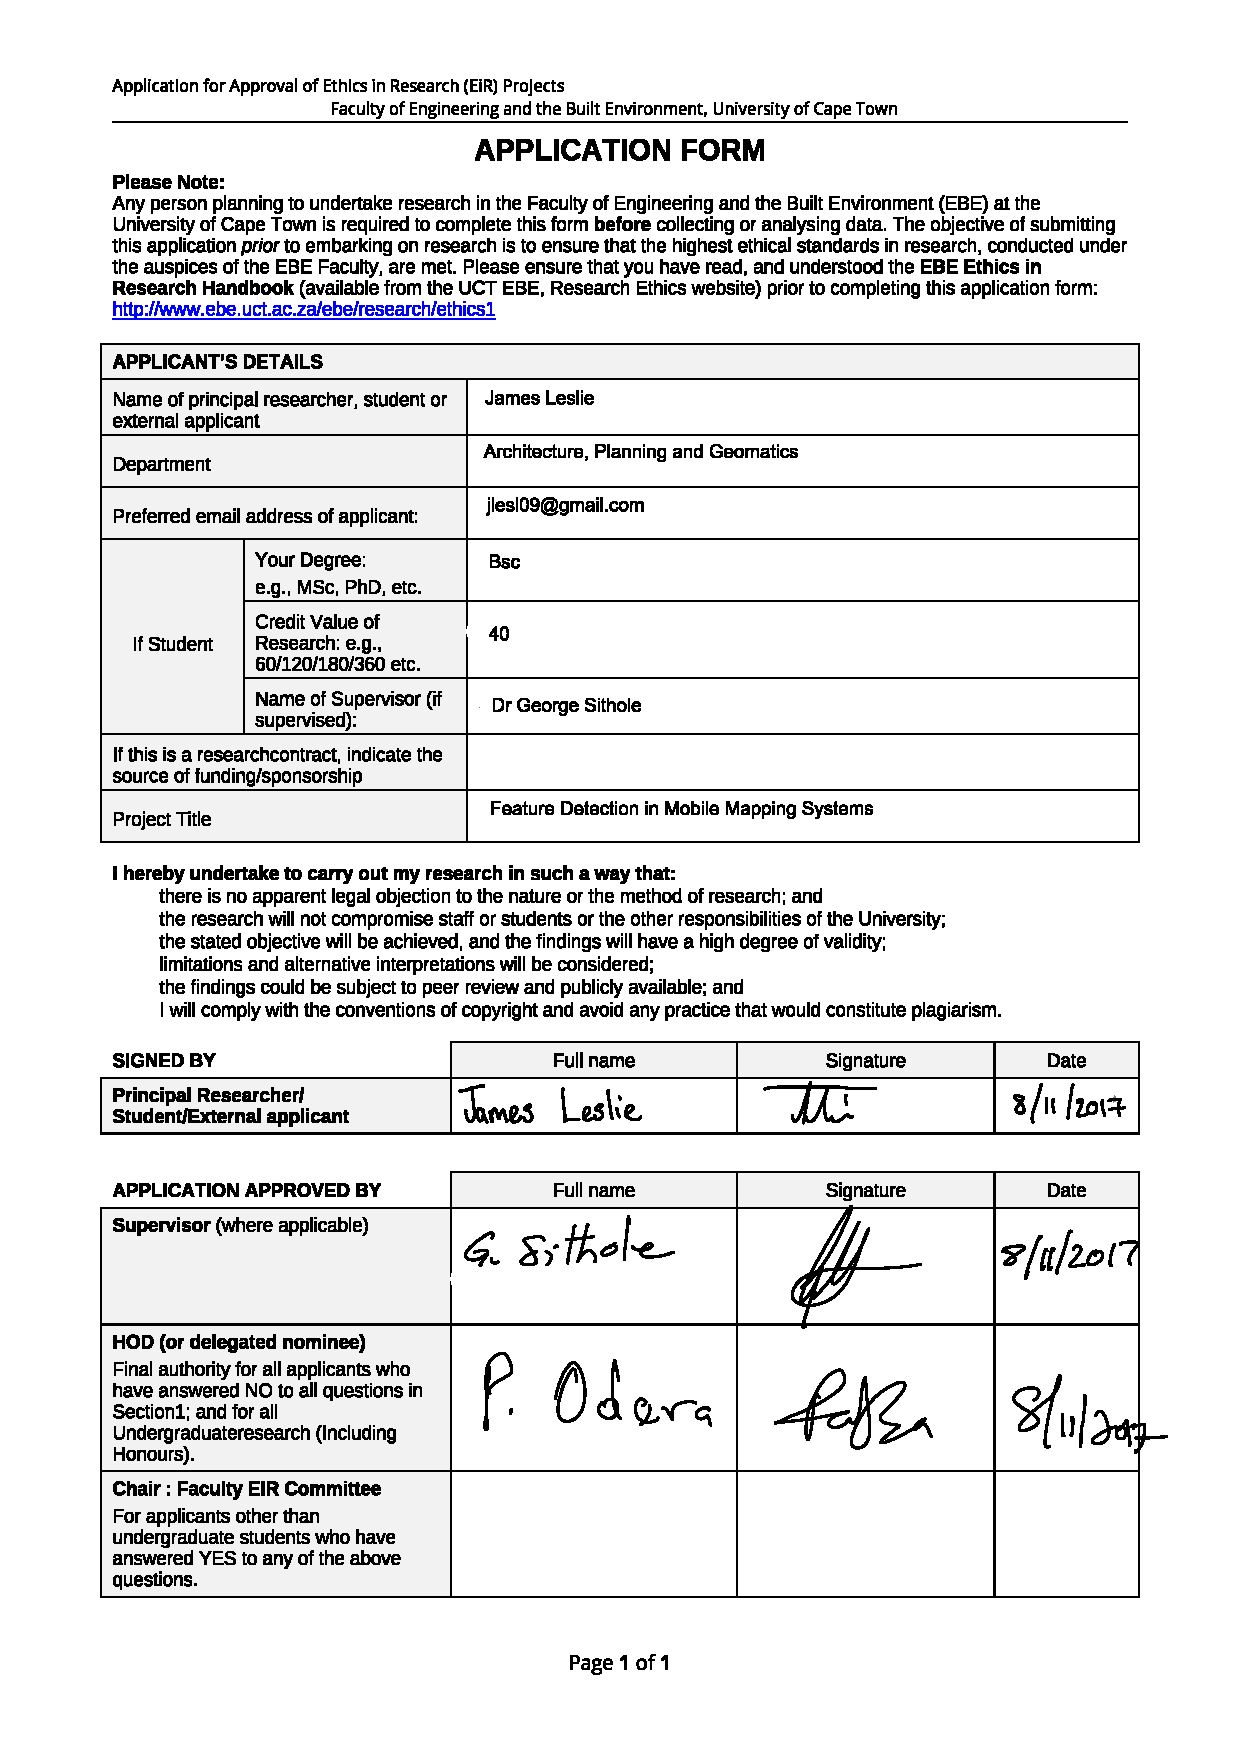
\includepdf[pages={1}]{Figures/0_Ethics.pdf}

%----------------------------------------------------------------------------------------
%	ABSTRACT PAGE
%----------------------------------------------------------------------------------------

\begin{abstract}
\addchaptertocentry{\abstractname} % Add the abstract to the table of contents
Recommender systems (RS) are used extensively in online retail and on media streaming platforms to help users filter the plethora of options at their disposal. Their goal is to provide users with suggestions of products or artworks that they might like.

Content-based RS's make use of user and/or item metadata to predict user preferences, while collaborative-filtering (CF) has proven to be an effective approach in tasks such as predicting movie or music preferences of users without using any data other than the interactions between users and items.

Latent factor models have have been used to achieve state-of-the-art accuracy in many CF settings, playing an especially large role in beating the benchmark set in the Netflix Prize in 2008. These models learn latent features for users and items to predict the preferences of users. The first latent factor models made use of matrix factorisation to learn latent factors, but recent approaches have made use of neural architectures with embedding layers.

This master's dissertation outlines collaborative genre tagging (CGT), a transfer learning application of CF that makes use of latent factors to predict genres of movies, using only explicit user ratings as model inputs.
\end{abstract}

%----------------------------------------------------------------------------------------
%	ACKNOWLEDGEMENTS
%----------------------------------------------------------------------------------------

\begin{acknowledgements}
\addchaptertocentry{\acknowledgementname} % Add the acknowledgements to the table of contents
I would like to give a sincere thank you to my project supervisor, Dr Miguel Lacerda. Without his guidance and direction, the result achieved in this project would not have been possible.
\end{acknowledgements}

%----------------------------------------------------------------------------------------
%	LIST OF CONTENTS/FIGURES/TABLES PAGES
%----------------------------------------------------------------------------------------

\tableofcontents % Prints the main table of contents

\listoffigures % Prints the list of figures

\listoftables % Prints the list of tables

%----------------------------------------------------------------------------------------
%	THESIS CONTENT - CHAPTERS
%----------------------------------------------------------------------------------------

\mainmatter % Begin numeric (1,2,3...) page numbering

\pagestyle{thesis} % Return the page headers back to the "thesis" style

% Include the chapters of the thesis as separate files from the Chapters folder
% Uncomment the lines as you write the chapters


\chapter{Introduction}

\label{intro} % For referencing the chapter elsewhere, use \ref{intro} 

\section{Problem Description}
The purpose of a  recommender system is to help people make decisions in an area where they do not necessarily have a wealth of personal experience \parencite{rs_1.1_Resnick}. The output of a recommender system is usually in the form of a suggestion to the user, helping them to make decisions such as what items to buy, what music to listen to or what movie to rent \parencite{handbook_1.1_intro}.

As the world of online commerce grew with the internet boom of the '90s, shoppers were presented with an overwhelming number of options to choose from. The need arose for a means for users to filter through the multitude of options to find the offerings most relevant to them \parencite{handbook_1.1_intro}.

As the number of options grew, so too did the amount of user feedback data. Already in 2007, the online video subscription service Netflix had collected nearly 2 billion ratings from more than 11.7 million subscribers on over 85 thousand titles in its first 10 years of operating. Considering the number of similar streaming and online commerce services, there is indeed an overwhelming number of options for users to choose from -- but also a wealth of data recommender systems can use to make suggestions \parencite{netflix_description}.

More choices means more feedback, we now have more recorded interactions of what people do -- and \textit{don't} -- like than ever before.

Much of these data are low-dimensional, typically containing only two or three attributes for each interaction, namely the user and item IDs and (optionally) a rating. This type of low-dimensional data is what separates recommender models from typical machine learning applications and is the focus of a specific type of approach to recommender system, known as collaborative filtering \parencite{cf_1.5_explicit}.

\section{Background to Research}
The Netflix Prize contest in 2008 paved the way for large improvements to the state of the art for predictive ability in collaborative filtering models \parencite{netflix_description}. The contest saw the progression from simpler k-nearest-neighbour models to the use of more advanced latent factor models, achieving a reduction of 10\% in the root mean squared error compared to the previous state of the art \parencite{netflix_bellkor}.

Despite the advances made during the contest, the timing of these efforts was untimely as this was before the mainstream adoption of deep learning. Four years after the close of the Netflix Prize contest "AlexNet", utilising the enhanced computational capacity of GPUs for model training, showcased the predictive ability of neural networks with its record-breaking accuracy in the annual ImageNet image classification contest \parencite{krizhevsky2012imagenet}. Since then, the field of deep learning has continued to grow, with neural networks achieving state-of-the-art accuracy on a wide range of problems \parencite{alom2018history}.

This project seeks to revisit the advances made by the contestants of the Netflix Prize and compare their results to those achievable with more modern deep learning approaches.

\section{Purpose of the Research}


\section{Layout of the Paper}
The literature review provides an overview of the relevant literature on recommender systems. The chapter covers the methodology surrounding the evaluation of recommender systems and outlines the two main types of models, namely content-based and collaborative filtering models. Particular attention is given to collaborative filtering models applied to explicit feedback data, leading to an in-depth discussion of the models that have been developed to perform this task on explicit feedback data.

Chapter 3 ...

Chapter 4 ...

Chapter 5 ...

Conclusions and recommendations for further research are outlined in Chapter 6


 
\chapter{Literature Review}
\label{lit_review} % For referencing the chapter elsewhere, use \ref{intro} 
This chapter provides a review of all related works in the field of recommender systems. The chapter first focuses on the background and origin of recommender systems and outlines their main applications. This is then followed by an overview of the methods used to evaluated the accuracy and effectiveness of recommender systems. Then, the two main categories of approaches to recommender systems are discussed, namely \textit{content-based} and \textit{collaborative filtering} systems. Finally, the chapter is concluded by evaluating the top submissions to the Netflix Prize, a contest that was held in 2008, which was a major event in the progression of collaborative filtering algorithms.

\section{Introduction to Recommender Systems}
As the world has become more digitally connected, people too have become connected to an increasing number of options. When trying to decide on what movie to watch, or what album to listen to, people are presented with a vast number of options that can, oftentimes, be overwhelming. To help people in making decisions such as these, inspiration is often taken from friends' word of mouth, reviews from critics, or general surveys. Recommender systems provide an automated means for helping people discover new items \parencite{rs_1.1_Resnick}.

The goal of a recommender system can be defined as predicting the response of a user for new items, based on historical information, and suggesting novel and/or original items for which the estimated response is positive \parencite{handbook_1.4_neighbourhood}.

\subsection*{Approaches to Recommender Systems}
Recommender systems can be divided into two broad categories. \textbf{Content-based} recommender systems make use of meta data for generating recommendations. Examples of item meta data include the genre of a musical artist or song, or the director of a movie. For users, meta data such as demographic information might be used. This meta data is used to match users to items based on matching tags - the recommendations for a user who likes work of a certain author, for example, might include other books by the same author or books of the same genre \parencite{di2012linked}.

There have been a number of successful content-based recommender systems. Many web recommenders use a keyword-based technique to match web pages based on the frequency of words on the page. In movie and book recommenders, a common approach is to use similarities between the text descriptions to match products. \parencite{handbook_1.3_content-based}

One major obstacle to content-based approaches is the lack of sufficient meta data, which can be time-consuming and costly to collect. \parencite{cf_1.6_implicit}

An alternative approach, known as \textbf{collaborative filtering} (CF), uses only the historical interaction behaviour between users and items to make recommendations \parencite{cf_1.1}. This is the approach that will be investigated in this project and will be described in more detail below.

\section{Evaluating Recommender Systems}
Before expanding on the intricacies of collaborative filtering, it is first necessary to discuss the methods and metrics that are commonly used to evaluate recommender systems. This is the most subjective aspect of the process, since the success of the system depends on the objectives of its designer. For example, the intent could be to stretch customer spend, or it could be to encourage users to discover new products. In each of these cases, success would be measured using different yard sticks \parencite{eval_colab}.

There are three main approaches for evaluating the success of a recommender system. The first approach is to evaluate the system offline, without any form of user testing. The other two approaches involve user testing; either using small groups of subject matter experts, or a more large-scale approach using online user testing. While each recommender system can be evaluated subjectively based on its ability to meet certain outcomes, there are certain measurable properties which can be used to compare different systems \parencite{handbook_1.8_evaluation}. The intended outcomes of the recommender system will determine whether it can be evaluated offline, or if it will require expert or user group online testing.

\subsection{Offline Evaluation}
Most recommender systems are scored and assessed on their ability to predict known user ratings. In this case, the models have been trained to predict the numeric values of ratings that users will assign to items. The predicted values can be compared to the true ratings using common regression metrics such as mean absolute error (MAE) or root mean square error (RMSE) \parencite{eval_coverage}. If we use $P$ and $O$ to denote the ordered sets of predicted and observed user ratings respectively, and $n$ to represent the total number of user-item interactions, then the accuracy of the recommender system can be measured as

\begin{equation}
    \text{MAE} = \dfrac{|P - O|}{n}
\end{equation}
or
\begin{equation}
    \text{RMSE} = \sqrt{\dfrac{(P - O)^{2}}{n}}.
\end{equation}

However, there are alternative metrics that aim to better reflect the quality perceived by users of the system \parencite{eval_colab}.

Prediction \textbf{coverage} provides a measure of how well the recommender system is able to encourage users to explore all of the item space. If $I$ is used to denote all items available to users and $I_p$ to denote all items recommended by the recommender system, then coverage can be measured as

\begin{equation} \label{eqn:cov}
    \text{coverage} = \dfrac{|I_p|}{|I|},
\end{equation}
which is the total number of items recommended by the system divided by the total number of items contained in the training data \parencite{eval_coverage}.

In some cases, a recommender system could achieve high levels of both accuracy and coverage, but still struggle to recommend new items to users. \cite{eval_colab} used the example of a recommender system that suggests bananas to shoppers in a grocery store: \textit{"Statistically, this recommendation is highly accurate: almost everyone buys bananas. However, everyone who comes to a grocery store to shop has bought bananas in the past, and knows whether or not they want to purchase more. Further, grocery store managers already know that bananas are popular, and have already organised their store so people cannot avoid going past the bananas."} 

It should be noted, however, that a recommender system should not \textit{only} recommend unexpected items. As \cite{swearingen2001beyondalgorithms} showed, non-novel recommendations help to develop trust from users in the system and should be combined with more unexpected suggestions to provide an enjoyable overall user experience.

\textbf{Serendipity} is a metric that has been used to assess both a recommendation's unexpectedness \textbf{and} its usefulness \parencite{online_predicting}. Serendipity is more of a conceptual evaluative measure, rather than a fixed formula like RMSE. One approach to capture serendipity numerically has been suggested by \parencite{eval_colab}. In the case where a recommender can produce expected probabilities for a given user for every item in the system, fir example, one could divide each probability by the average user probability score to produce re-weighted scores. The resulting probabilities would represent a measure of how much more likely a given user is to like items than the average user.

In the case where ratings are not available -- that is when only a list of user-item interactions is given -- the task of providing recommendations is often transformed into one of providing a set number of items to a user. Using $P$ to denote the set of items that are suggested to the user and $O$ to denote the set of items which the user was observed to have preferred, this type of approach can then be evaluated using \textbf{precision} and \textbf{recall}, computed as

\begin{equation}
    \text{precision} = \dfrac{|P \cup O|}{|P|}
\end{equation}
and
\begin{equation}
    \text{recall} = \dfrac{|P \cup O|}{|O|}
\end{equation}
\parencite{handbook_1.4_neighbourhood}.

\subsection{Online Testing}
Testing recommender systems in an online manner, be it user studies or large-scale trials, requires a large enough audience that can be split into test and control groups. Ideally, the two user groups would be identical apart from the fact that the test group would receive suggestions from the recommender system, while the control group would not. The two groups would then be assessed on their behaviour over a trial period, allowing for the recommender system to be assessed in various areas such as uplift in incremental sales or exploration of the item space \parencite{online_predicting}.

An example of online testing can be found in the work done by \cite{swearingen2001beyondalgorithms}, where users were asked to evaluate a number of internet recommender systems and compare their suggestions to those of their friends. Users were asked to classify which recommendations they received were good, and then to further distinguish between \textbf{useful} recommendations they had never seen before and \textbf{previously liked} recommendations. One particularly interesting observation from this study was that recommender systems tended to produce more suggestions of completely new items than friends, who tended to recommend items of which users were already aware.

The advantage of testing recommender systems in this way is that it affords the systems the chance to influence a user's interaction behaviour. Indeed, recommender systems exist for the main purpose of suggesting items to users that they are predicted to like, but would otherwise not have known about. The influence of a recommender system cannot be assessed through back-testing. It can only be done through online trials \parencite{handbook_1.4_neighbourhood}.

Since each system needs its own independent test group, the size of the audience required only increases with the number of recommender systems being compared, which makes online testing infeasible in the context of this master's dissertation. Therefore, all comparisons between recommender systems in this paper will be made using offline metrics.

\subsection{Netflix Prize}
A major event in the progression of recommender system methods, as well as the evaluative metrics thereof, was the 2006 Netflix Prize. In 2019, Netflix is a well-known online video subscription service that provides content to subscribers through streaming. However, in 2006 Netflix was an online video subscription service that provided DVD rentals to subscribers via the mail. As part of their service, they encouraged users to rate movies that they watched which resulted in the creation of a data set of some 1.9 billion ratings from 11.7 million subscribers across 85 thousand titles in under 10 years \parencite{netflix_description}.

This data set was used by Netflix to create their own recommendation algorithm, which was known as Cinematch. Cinematch used a variant of Pearson's correlation to determine a movie's similarity to all other movies. These similarities between movies were used to provide personalised recommendations to users based on the movies they had rated. The main method used to assess the performance of Cinematch was to compute the RMSE between the predicted and observed user ratings \parencite{netflix_description}.

In 2006, Netflix released a variation of this data set to the data science community at large with the challenge of improving on the performance achieved by the existing Cinematch algorithm. The data set provided for this challenge contained over 100 million ratings (and their dates) from over 480 thousand subscribers on almost 18 thousand movies. The data were collected between 1998 and 2005, and comprised a representative sample of all ratings captured by Netflix during this period. The user ratings were measured on an integer scale from 1 to 5. Three million of the most recent ratings from those same subscribers across the same set of movies was withheld as a competition qualifying set. Half of the qualifying data set was used to compute the RMSE of submissions onto the running public leader board, while the other half, known as the "quiz" subset was used by Netflix to decide the eventual winning team \parencite{netflix_description}.

As a reference for competition contestants, Netflix reported that the Cinematch algorithm was able to achieve a performance of 0.9514 RMSE on the quiz subset, which was 9.6\% lower than simply predicting using the average movie ratings \parencite{netflix_description}.

Figure \ref{fig:netflix_submissions} shows the relative distribution of the submissions' performance with respect to that of the Cinematch algorithm. The figure was created in 2007, at which point no team had achieved the goal of a 10\% improvement over Cinematch. The numbers in red correspond to submissions in which the same value is used for every prediction, while the "wooden spoon" was the lowest score achieved by any of the entrants. Interestingly, a significant number of submissions achieved RMSE scores lower than would be achieved by predicting every rating to be 4.

\begin{figure}[H]
\centering
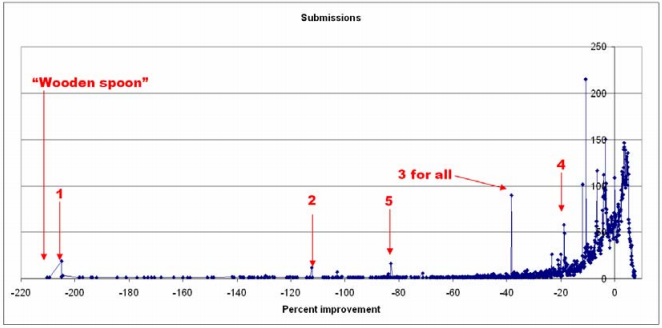
\includegraphics[width=13cm]{Figures/2_1_netflix-prize.png}
\decoRule
\caption[Netflix submissions]{Netflix prize submissions ordered by improvement over Cinematch \parencite{netflix_description}.}
\label{fig:netflix_submissions}
\end{figure}

However, in 2008, the competition reached its conclusion, when the team known as "BellKor's Pragmatic Chaos" surpassed the 10\% improvement level \parencite{netflix_bellkor}.

\section{Collaborative Filtering}
The term ``collaborative filtering'' was first coined by \cite{cf_1.3_origin}, who used it to refer to a system for suggesting relevant emails for a person from a selection of mailing lists. This system incorporated the reactions of other users in the filtering process.

Since then, the term has generally been used to describe a process through which known preferences of users in a group are used to predict the unknown preferences of other users \parencite{cf_1.1}. In most cases, the preferences of users within the group are indicated by a rating or score of some kind; for example, users might assign positive ratings to items they liked, and negative ratings to items they did not. The term \textit{collaborative} refers to the fact that the users of the system improve its performance with each rating that they contribute \parencite{cf_1.2_eigentaste}, i.e., as users record more ratings of items, the ability of the system to \textit{filter} accurate recommendations for other users improves. 

Collaborative filtering techniques provide an algorithmic method for making recommendations to users, based on the preferences of other similar users. The fundamental assumption that underlies CF techniques is that users who have rated $k$ items similarly will also rate other items similarly. For example, if user $A$ likes movies $m_1$, $m_2$, $m_3$, and user $B$ likes movies $m_1$, $m_2$, $m_3$, $m_4$, then user $A$ is also likely to enjoy movie $m_4$ \parencite{cf_1.1}.

One of the advantages of collaborative filtering is that it can be performed without any meta data relating to either the users or the items in the database. Whereas other predictive models make predictions for a response variable using the values of one or more predictor variables, CF models make predictions for ratings using only other ratings \parencite{handbook_1.1_intro}.

One issue with content-based approaches is their limited capacity to recommend novel, unexpected items. The system will recommend items which match highly to a user's known preferences, i.e. they are limited by the user's tendency for exploration. \parencite{handbook_1.3_content-based}

Collaborative-filtering-based models, on the other hand, leverage the collective experiences of all users to recommend interesting new items to users. In contrast to content-based models, models that employ collaborative filtering are known to produce serendipitous recommendations that users would not typically expect \parencite{herlocker2002empirical}.

\subsection{User Feedback}
 In collaborative filtering recommender systems, the inputs are provided by people (users) who rate items with which they have interacted \parencite{cf_1.5_explicit}. The function of a recommender system is to aggregate these ratings from users to make recommendations to other users on which items they might like. In some cases, ratings are provided to a recommender system explicitly by users, but in many other cases these ratings have to be inferred based on user-item interactions \parencite{cf_1.6_implicit}. 

\subsubsection{Explicit Ratings}
Explicit feedback is captured when a user makes the conscious decision to \textit{explicitly} rate an item. These ratings can be binary (e.g.\ like or dislike), numeric (e.g.\ 1-10 rating scale) or unstructured (e.g.\ annotated text). For example, a user can indicate that they like a certain song by giving it a "thumbs up" on a music streaming service \parencite{cf_1.5_explicit}.

This type of feedback directly captures user preferences towards items; however, it can be scarce. It has also been found that the rate at which users provide explicit feedback decreases over time and, furthermore, that leaving feedback has a negative effect on user behaviour overall \parencite{cf_1.5_explicit}. This is shown in figure \ref{fig:playcount} where the average percentage of loved tracks over all users is shown to decrease as playcount increases.

\begin{figure}[H]
\centering
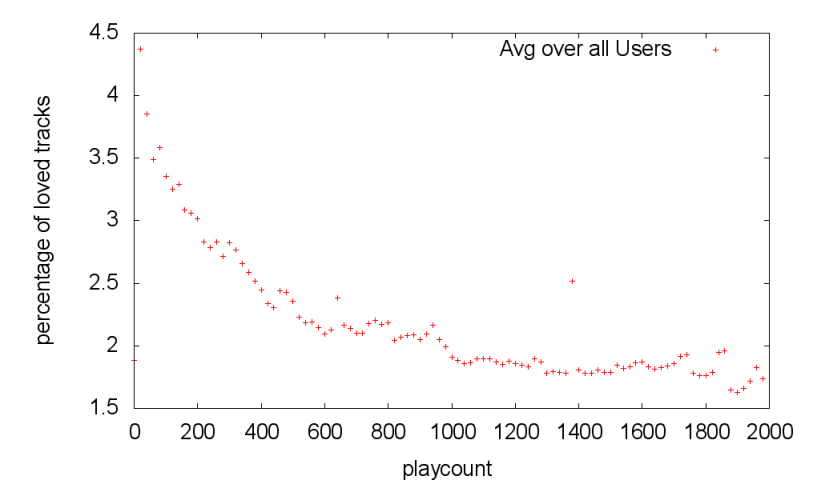
\includegraphics[width=13cm]{Figures/2_2_playcount-vs-loved.png}
\decoRule
\caption[Playcount-loved]{Percentage of loved tracks as playcount increases \parencite{cf_1.5_explicit}.}
\label{fig:playcount}
\end{figure}

\subsubsection{Implicit Feedback}
Alternatively, the user might not explicitly rate items they like, in which case a recommender system would need to infer their preferences from their interaction history. Using the example of a music streaming service, many users do not choose to 'like' or rate songs; however, they will tend to listen to songs they like more often than those they do not. \cite{cf_1.5_explicit}, showed that there is a positive correlation between the number of 'likes' a track receives from users and its total play count. Therefore, it is a viable option to infer positive feedback from user interaction data. Other forms of implicit feedback include purchase history, browsing and search patterns, or mouse movements and click patterns \parencite{handbook_1.5_cf}.

Whether the user feedback is implicit or explicit, the job of the recommender system is the same - to aggregate this feedback from users to aid others in discovering new items of interest. It has been shown that using a combination of explicit and implicit feedback can yield improved recommendation accuracy \parencite{cf_1.4_comparison}; however, it is the subtleties around \textit{how} recommender systems identify all the signals from the available user feedback data that remains the greatest area of focus for improving accuracies.

\subsection{Neighbourhood-based Recommender Models}
There are two main techniques used in collaborative filtering recommender systems: \textit{neighbourhood-based} and \textit{latent factor} models \parencite{handbook_1.5_cf}. As the name suggests, neighbourhood models employ a nearest-neighbours approach to recommending items to users.

Neighbourhood-based approaches were some of the most prevalent in the early years of recommender systems at the end of the 90s. These methods make use of similarity measures to select subsets -- or neighbourhoods -- of users or items \parencite{cf_1.6_implicit}. These neighbourhoods are used to produce weighted average ratings to generate predictions for users \parencite{herlocker1999algorithmic}.

\subsubsection{User-based similarity}
The first types of neighbourhood models estimated unknown ratings using a user-oriented approach in which predictions were based on the known ratings of like-minded users \parencite{cf_1.6_implicit}.

To make a prediction for a given user $a$ for item $i$, the first step is to measure their similarities to all other users of the system. Similarity between users $a$ and $u$ can be calculated using the Pearson correlation coefficient, $w_{a,u}$, computed as
\begin{equation}
    w_{a,u} = \dfrac{\sum\limits_{i=1}^{m}[(r_{a,i}-\bar{r}_a)(r_{u,i}-\bar{r}_u)]}{\sqrt{\sum\limits_{i=1}^{m}(r_{a,i}-\bar{r}_a)^2\sum\limits_{i=1}^{m}(r_{u,i}-\bar{r}_u)^2}},
\end{equation}
where $r_{a,i}$ is the rating for the active user $a$ of item $i$ and $\bar{r}_a$ is their average rating, while $m$ is the set of items covered by either user.

This similarity can then be used to predict the rating for the active user for item $i$ as
\begin{equation}
    P_{a,i} = \bar{r}_a + \dfrac{\sum\limits_{u \in N(a)}w_{a,u}(r_{u,i}-\bar{r}_u)}{\sum\limits_{u \in N(a)}w_{a,u}},
\end{equation}
where $N(a)$ is the set of user $a$'s neighbours \parencite{herlocker2002empirical}.

This approach was modified by \cite{shardanand1995social}, who used a constrained Pearson correlation coefficient, calculated as
\begin{equation}
    w_{a,u} = \dfrac{\sum\limits_{i=1}^{m}[(r_{a,i}-4)(r_{u,i}-4)]}{\sqrt{\sum\limits_{i=1}^{m}(r_{a,i}-4)^2\sum\limits_{i=1}^{m}(r_{u,i}-4)^2}}.
\end{equation}
The value 4 was used as it was the midpoint of the seven-point rating scale on which their music recommendation system, dubbed "The Ringo", was based. The number of neighbours was limited by applying a correlation threshold, where only users above the threshold could be considered for membership to the neighbourhood. Increasing the magnitude of this threshold resulted in greater accuracy, but limits the number of items for which the system can make recommendations \parencite{herlocker2002empirical}.

The most common alternative similarity measure to the Pearson correlation coefficient is the cosine similarity, which is calculated between users $a$ and $u$ as
\begin{equation}
    \cos(r_a,r_u) = \dfrac{(r_a\cdot r_u)}{||r_a||\times||r_u||},
\end{equation}
where $a$ and $u$ represent the ratings vectors for each user, considering only items which have been rated by both users, $r_a\cdot r_u$ is the dot product of the two rating vectors and $||r_a||\times||r_u||$ is the product of their magnitudes \parencite{handbook_ch2}.

This measure can then be used to make a prediction for user $a$ and item $i$ by selecting the $n$ most similar neighbours and taking an average of their rating of the item, weighted by their cosine similarity.

Though the Pearson correlation and cosine similarity are the most popular measures used, it is possible to use any other common distance measure, such as the Euclidean or Minkowski distance \parencite{handbook_ch2}.

\subsubsection{Item-based similarity}
An alternative to neighbourhood models is an item-oriented approach, in which the known ratings of a user for similar items are used to make a prediction for a new item \parencite{cf_1.6_implicit}. When making a prediction for user $a$ and item $i$, all known ratings of the user are used as the neighbourhood. The predicted rating is taken as the average of all known ratings, weighted by their corresponding item similarity with $i$. The similarity measure for this neighbourhood can be any of the same measures as used in the user-based approach, only in this case the similarities are measured between items instead of users \parencite{handbook_1.4_neighbourhood}.

\subsection{Latent Factor Recommender Models}
Latent factor models attempt to characterise both users and items using anywhere in the region of between 20 to 100 factors. These latent factors capture behavioural patterns between users and items in the ratings space \parencite{koren2009matrix}.

The most common version of latent factor model is the matrix factorisation (MF) method, used by \cite{bellkor_2008} to win the Netflix Prize. In this approach, the user/item interaction data is represented as a matrix which is then factorised as the product of two lower rank matrices. 

Figure \ref{fig:2_matrix-decomposition} shows the matrix representation of the explicit interactions between users and items. All blue values are known ratings submitted by users, while the white zeroes represent unknown values which need to be predicted. Each row thus holds the ratings made by a particular user and each column the ratings received by a single item. The rating made by user $i$ of item $j$ can be found in the $j^{th}$ column of row $i$.

\begin{figure}[H]
\centering
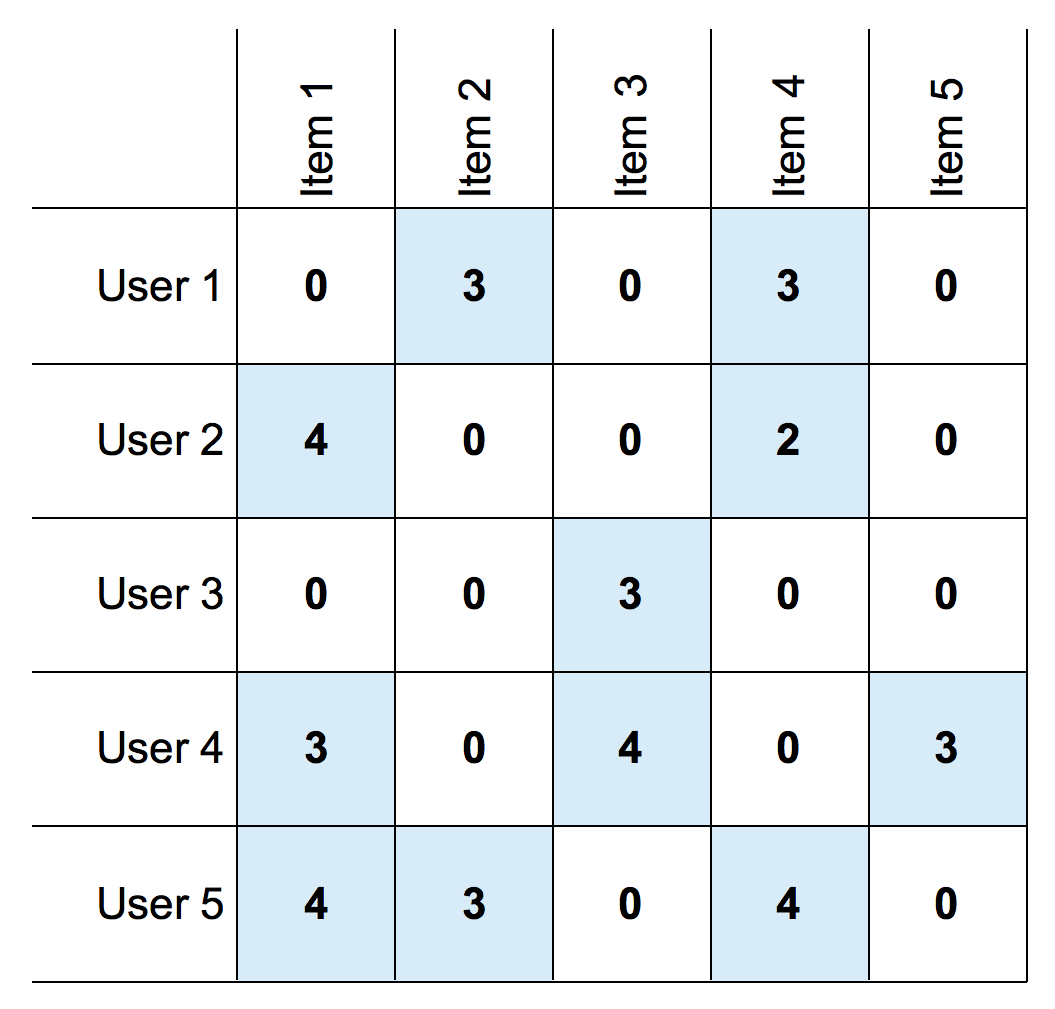
\includegraphics[width=6cm]{Figures/2_3_matrix.png}
\decoRule
\caption[Ratings matrix]{Interactions between users and items represented as a matrix \parencite{bailey_2016}.}
\label{fig:2_matrix-decomposition}
\end{figure}

If the ratings matrix consists of $m$ rows and $n$ columns, then any two matrices of dimensions $m$ x $d$ and $n$ x $d$ respectively, when cross multiplied together, would result in a matrix of the same dimensions as the original ratings matrix. The common dimension, $d$, is a hyperparameter which represents the number of latent factors, where $d <= \min(m,n)$ \parencite{bailey_2016}.

\begin{figure}[H]
\centering
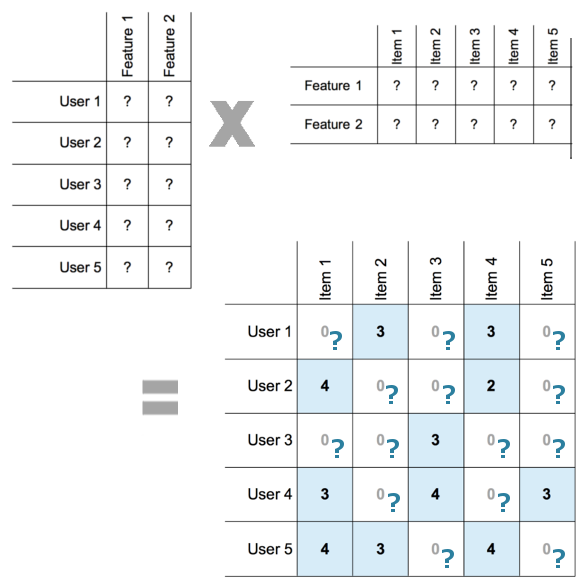
\includegraphics[width=9.5cm]{Figures/2_4_matrix_factorization.png}
\decoRule
\caption[Matrix decomposition]{Ratings matrix factorised as product of two latent factor matrices \parencite{bailey_2016}.}
\label{fig:factors}
\end{figure}

To get the rating for the first user of the first movie, one takes the dot product of the first row of the user matrix with the first column of the item matrix. More generally, the rating made by user $i$ of item $j$ is calculated as

\begin{equation}
    \hat{r}_{ij} = p_i \cdot q_j^T,
\label{eqn:dot_prod}
\end{equation}

where $p_i$ is the $i^{th}$ row of the user latent factor matrix and $q_j$ is the $j^{th}$ column of the item latent factor matrix.

\subsubsection{Optimisation techniques}
The two latent factor matrices that are used in the MF approach need to be \textit{learnt}. Their values can be solved through either stochastic gradient descent or alternating least squares (ALS), optimising the minimal distance between the original ratings matrix and the reconstructed matrix. The ALS optimisation technique was the favoured approach taken by \cite{bellkor_2008}. This technique holds the values in one factor matrix fixed and then uses least squares to solve the values in the other and \textit{vice versa}. The converged solution provides the closest reconstruction of the original ratings matrix, with the missing values filled in \parencite{koren2009matrix}.

The two resulting latent factor matrices consist of vectors which describe both the users and the items respectively. For each user and item, there will be $d$ latent factors which represent their characteristics. In the case that the items are movies, the latent factors might represent known dimensions, like genres such as comedy or romance. They might also represent deeper dimensions, like dialogue style or the amount of satire. The latent factors might also represent completely uninterpretable dimensions too. In the case of users, the latent factors represent their partiality to the corresponding item latent factor \parencite{koren2009matrix}.




\subsubsection{Biases}
The MF approach may be extended to include biases which compensate for systematic tendencies across both users and items. For example, some users tend to rate all items higher or lower than average, and some items might be generally over-rated by all users \parencite{koren2009matrix}.

When incorporating biases, equation \ref{eqn:dot_prod} becomes
\begin{equation}
    \hat{r}_{ij} = \mu + b_i + b_j + p_i \cdot q_j^T,
\label{eqn:dot_bias}
\end{equation}
where $\mu$ is the overall average rating and $b_i$ and $b_j$ are the biases of user $i$ and item $j$.

\subsubsection{Netflix Prize winning submission}
The winning submission to the Netflix Prize made use of an ensemble model, achieving an RMSE of 0.8712 on the test set using a combined total of over 500 models which included MF, restricted Boltzmann machines and nearest neighbour models. Despite this extensive range of models used in their winning ensemble, the team members noted that the most accurate standalone approach was to use MF \parencite{netflix_bellkor}. 

Aside from the choice of algorithm(s), the winning team paid special attention to what they termed "baseline predictors". The purpose of these was to "encapsulate those effects which do not involve user-item interaction." This method meant that predicted ratings were decomposed into multiple parts and is not dissimilar to how equation \ref{eqn:dot_bias} represents predicted ratings. In this equation, the first three terms can be considered baseline features, while the final term, $q_i^T p_u$, represents the specific user-item interaction. For example when predicting how a user, Alice, might rate the movie Inception, the prediction would first consider the average rating of the movie, as well as the average of all of Alice's ratings as the baseline predictors. Then, the specific user-item interaction is made using the latent features and is used to adjust the baseline prediction. In addition to user and item biases, temporal aspects were used to adjust the baseline. Factors such as time since a user's first rating and how many ratings a user made on a particular day were found to have a significant impact on user ratings. To capture temporal effects, the user and item biases were each calculated as a function of time. 

When accounting for temporal components, equation \ref{eqn:dot_bias} becomes

\begin{equation}
    \hat{r}_{ui} = \mu + b_u(t_{ui}) + b_i(t_{ui}) + q_i^T p_u,
\label{eqn:temp_baseline}
\end{equation}

where $b_u$ and $b_i$ are functions that change over time \parencite{netflix_bellkor}.

\subsection{Uses of deep learning in collaborative filtering}
Tremendous effort was required from all of the contestants of the Netflix Prize competition to push the boundaries of predictive ability in CF models. Ensemble models and intricate modelling of baseline predictors were used to eek out marginally better models; however, it was shown that the improvement in accuracy was largely due to the use of latent factors. Then, it was through the use of matrix decomposition that these latent factors were learnt; however neural networks can perform the same task through the use of embedding layers, with the added ability of learning non-linear patterns in the data.

The first notable use of deep learning for collaborative filtering was in \cite*{sedhain2015autorec}, when \citeauthor{sedhain2015autorec} used an autoencoder framework for their \textit{AutoRec} model. They opted for an item-based approach in which the input to the neural network is a partially observed vector containing all user ratings for a given item. Figure \ref{fig:autorec-arch} shows the architecture of this model.

\begin{figure}[H]
\centering
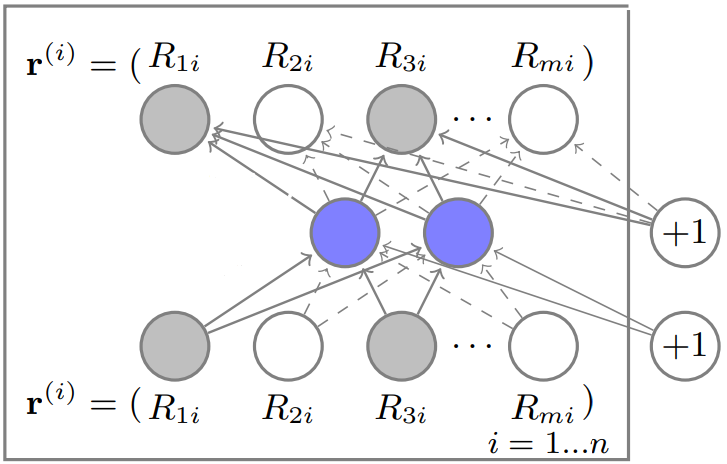
\includegraphics[width=8cm]{Figures/2_autoRec.png}
\decoRule
\caption[AutoRec]{AutoRecu uses an autoencoder architecture  \parencite{sedhain2015autorec}}
\label{fig:autorec-arch}
\end{figure}

It can be seen in figure \ref{fig:autorec-arch} that the input dimension of the AutoRec model is equal to the number of users, $m$. There are $n$ copies of the network, one for each item. Since each input is sparse, only the parameters associated with the observed ratings are updated during backpropagation. This means that the trained model takes as input a sparse item ratings vector, representing all available user ratings for that item, and outputs a complete ratings vector containing all predicted user ratings for the item \parencite{sedhain2015autorec}.

Evaluation of this model was done using the MovieLens 1M, 10M and Netflix datasets using 5 separate random 90\%-10\% train-test splits, with 10\% of the training data being used for hyperparameter tuning. Test accuracy was taken as the average of these 5 random splits and users or items in the test set without training observations were given a default rating of 3 stars. They reported test accuracies of 0.831, 0.782 and 0.823 on the MovieLens 1M, 10M and Netflix datasets respectively \parencite{sedhain2015autorec}.

Figure \ref{fig:autorec-arch} shows the item-based AutoRec model.
\citeauthor{sedhain2015autorec} experimented with a user-based model, taking $n$-dimensional user rating vectors as inputs to $m$ copies of the network. However, they found this model achieved reduced accuracy, likely due to the fact that there are more items per movie than per user in the datasets they used.

A neural architecture was used in the "Neural Collaborative Filtering" (NCF) model created by \cite{he2017neural}. This particular effort focused on the CF scenario where only implicit feedback is used; however, the architecture used is equally suited to using explicit feedback. Figure \ref{fig:ncf-arch} shows the architecture of a NCF model, with $X$ hidden units and $k$ latent factors.

\begin{figure}[H]
\centering
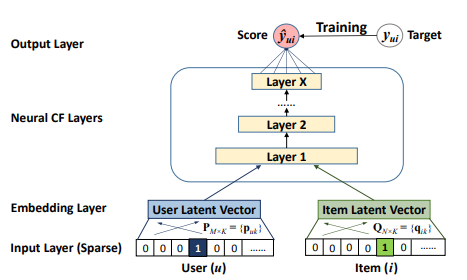
\includegraphics[width=9.5cm]{Figures/2_neural-cf.png}
\decoRule
\caption[Neural Collaborative Filtering]{Neural Collaborative Filtering architecture \parencite{he2017neural}}
\label{fig:ncf-arch}
\end{figure}

The NCF model generalises MF through the use of an embedding layer, which combines both user and item latent factors. The embedding layer serves the same purpose as the latent factor matrices in the MF approach, while the hidden layers allow for non-linear combinations of these latent factors when predicting ratings.

Although the results achieved by \citeauthor{sedhain2015autorec} represented an improvement of more than 5\% on the winning submission to the Netflix Prize, it should be noted that their method of evaluation on the Netflix set was not equivalent to the true holdout set used in the competition.

Finally: \parencite{rendle2019difficulty} and \parencite{dacrema2019we}.
\chapter{Data Description}
This chapter provides an overview of the four datasets used in this minor dissertation, all of which contain explicit ratings made by users across various item sets. Three of the datasets contain movie ratings, while the other contains ratings of books.

\section{Datasets}
The MovieLens (ML) datasets are used frequently in CF research efforts. GroupLens research at the University of Minnesota is responsible for maintaining these data. Three stable ML datasets were used in this project, each containing a different number of ratings: ML 100k (100 thousand ratings),  ML 1M (1 million ratings) and ML 10M (10 million ratings). The first two datasets use a 5 star, integer-only rating scale, while the 10M dataset contains ratings from 0.5 -- 5 stars, in increments of a half \parencite{harper2016movielens}.

The Goodbooks-10k dataset contains 10 thousand books, with a total of just under 6 million ratings made by over 50 thousand users \parencite{goodbooks2017}.

\section{Number of Users, Items and Ratings}
Each dataset has a different profile in terms of the ratios between numbers of users, items and ratings. The \textbf{density} is calculated as the number of ratings provided as a proportion of the total number of possible user-item interactions. ML 100k -- the dataset with the fewest ratings -- has 943 unique users and 1 682 unique movie titles. This would allow a total of 1 586 126 possible user-movie ratings. Since there are only 100 000 ratings in this dataset, its density is thus $100000/1586126 = 6.30\%$. Table \ref{tab:data-summary} provides a summary of the four datasets.

\begin{table}[H]
\centering
\begin{tabular}{c | c | c | c | c | c}
\toprule
\textbf{Name} & \textbf{Rating Scale} & \textbf{Users} & \textbf{Items} & \textbf{Ratings} & \textbf{Density} \\
\midrule
ML 100k & 1--5, stars & 943 & 1 682 & 100 000 & 6.30\% \\
ML 1M & 1--5, stars & 6 040 & 3 706 & 1 000 209 & 4.47\% \\
ML 10M & 0.5--5, half-stars & 69 878 & 10 681 & 10 000 054 & 1.34\% \\
Goodbooks-10k & 1--5, stars & 53 424 & 10 000 & 5 976 479 & 1.12\% \\
\bottomrule
\end{tabular}
\caption[Data summary]{Summary of the datasets used in this project}
\label{tab:data-summary}
\end{table}

ML 100k, 1M and the Goodbooks-10k sets all use an integer rating scale between 1 and 5 stars. The ML 10M set also uses a 5 star scale, but allows half star ratings.

In terms of size, ML 100k is the smallest with 100 thousand ratings, while the other sets all range between 1 and 10 million ratings. ML 10M contains the most items, albeit only by a slight margin over Goodbooks-10k.

\section{Distribution of Ratings}
Table \ref{tab:ratings-distribution} provides a summary of the distribution of ratings across users and items in each of the datasets.

All three MovieLens datasets have a minimum of 20 ratings per user, while some of the movies have only 1 rating.

The Goodbooks-10k dataset is similar to the MovieLens datasets in terms of its distribution across items; however, every book has at least 8 ratings as opposed to the 1 rating minimum of the MovieLens sets.

\begin{table}[H]
\centering
\begin{tabular}{c | c | c | c | c | c | c}
\toprule
\textbf{Name} & \textbf{Min User} & \textbf{Max User} & \textbf{Avg User} & \textbf{Min Item} & \textbf{Max Item} & \textbf{Avg Item} \\
\midrule
ML 100k & 20 & 737 & 106 & 1 & 583 & 60 \\
ML 1M & 20 & 2 314 & 166 & 1 & 3 428 & 270 \\
ML 10M & 20 & 7 359 & 143 & 1 & 34 864 & 937 \\
Goodbooks-10k & 19 & 200 & 112 & 8 & 22 806 & 598 \\
\bottomrule
\end{tabular}
\caption[Ratings distribution]{Summary of the distribution of ratings in each dataset}
\label{tab:ratings-distribution}
\end{table}

\subsection{Number of Ratings per User}
All three MovieLens datasets have a similar right-tailed distribution of the number of ratings made per user. The majority of users have made a small number of ratings -- between 1 and 100 -- with a small number of users having rated a very high number of movies.

The Goodbooks-10k dataset user ratings follow a bell-shaped distribution, with the majority of users having rated between 75 and 130 books. No user has rated fewer than 19, or more than 200, books.

The histograms in figures \ref{fig:ML10M-users} and \ref{fig:goodbooks-users} show the distributions of the number of ratings made per user in ML 10M and Goodbooks-10k. MovieLens 1M and 100k have similar shapes, albeit each with fewer users than the ML 10M shown in figure \ref{fig:ML10M-users}.

\begin{figure}[H]
\centering
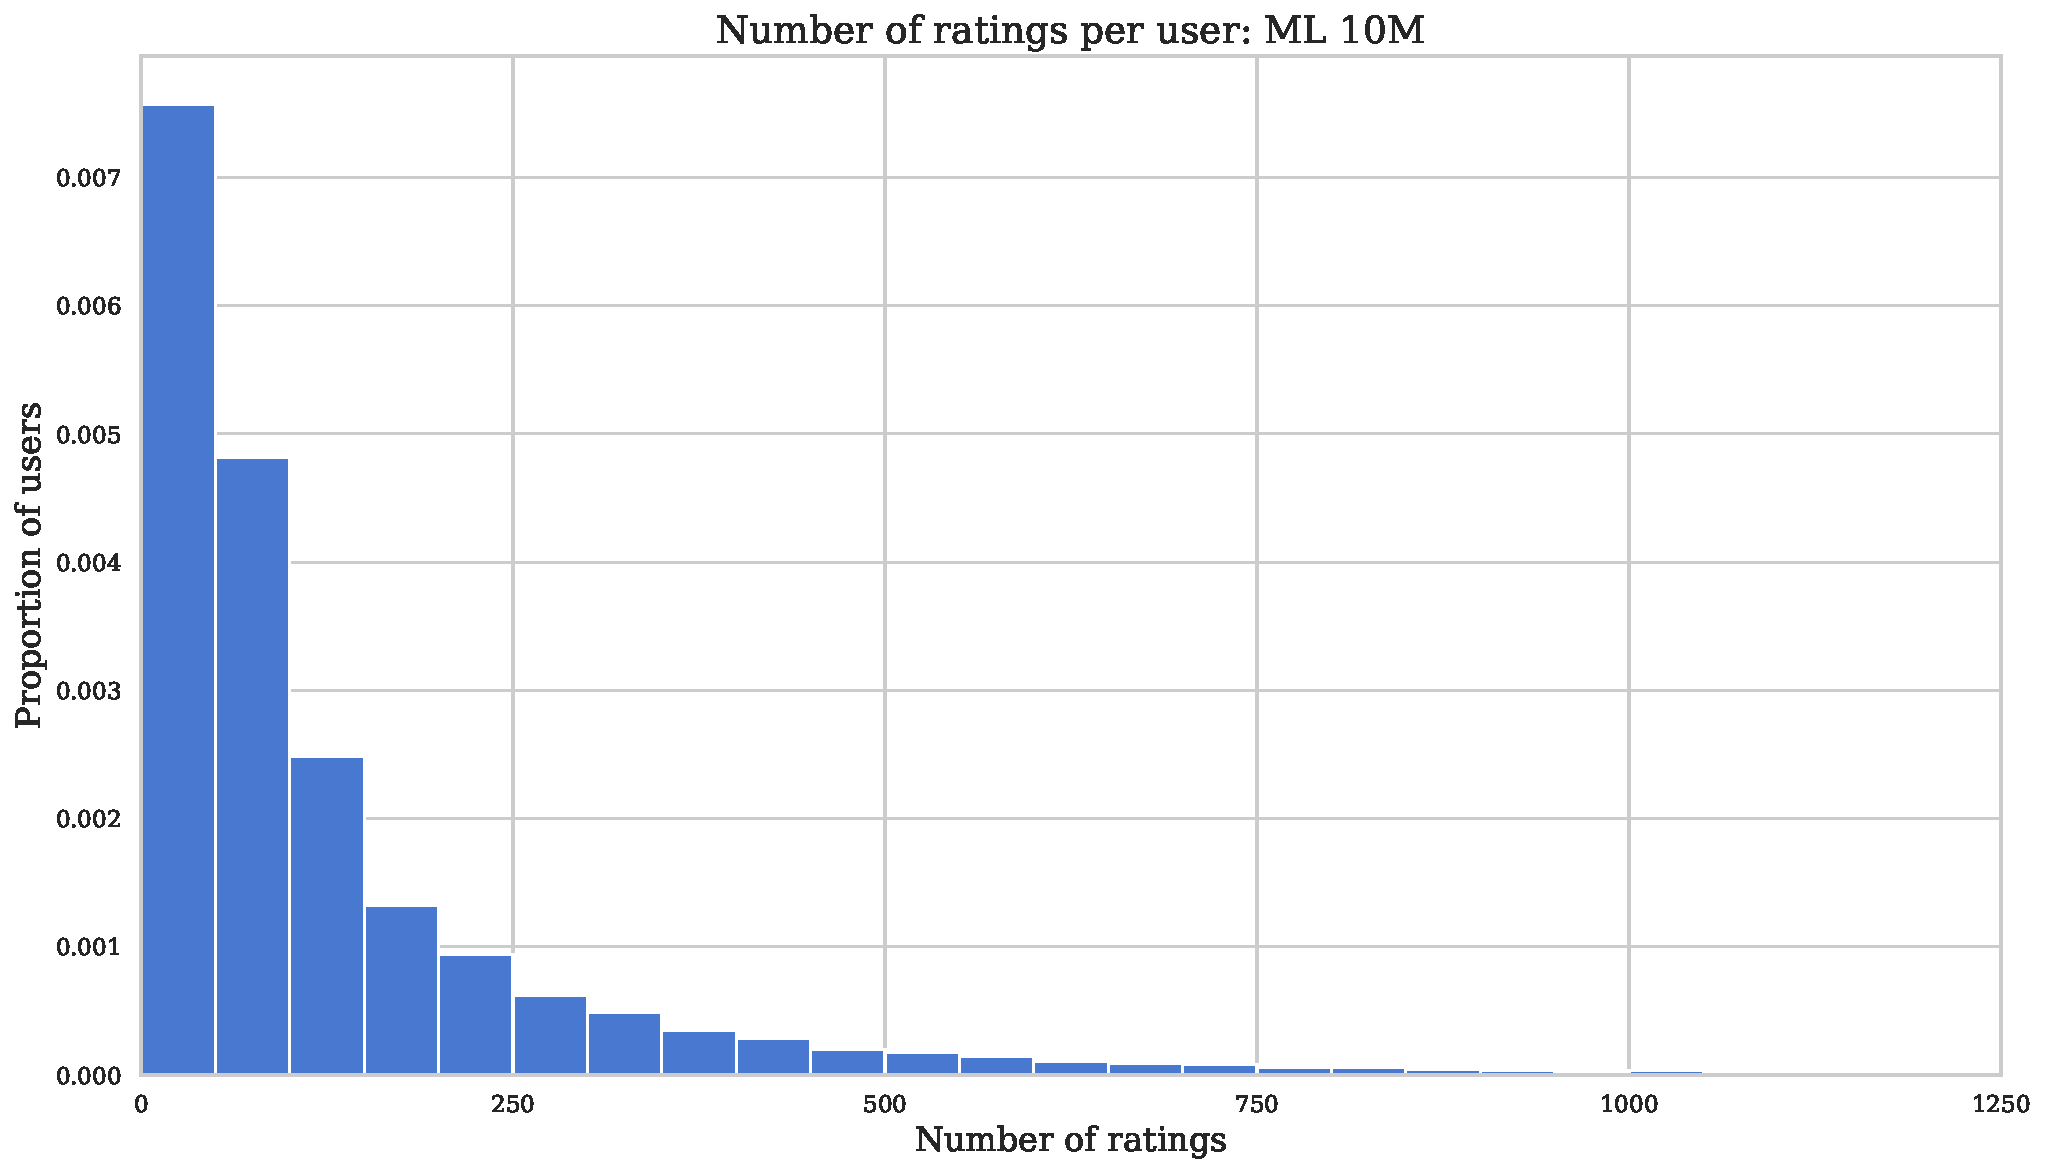
\includegraphics[width=0.75\textwidth]{Figures/3_ratings-distributions/ml_10m_user-ratings.pdf}
\caption{ML 10M number of ratings per user. Most users have rated a small number of movies.}
\label{fig:ML10M-users}
\end{figure}

\begin{figure}[H]
\centering
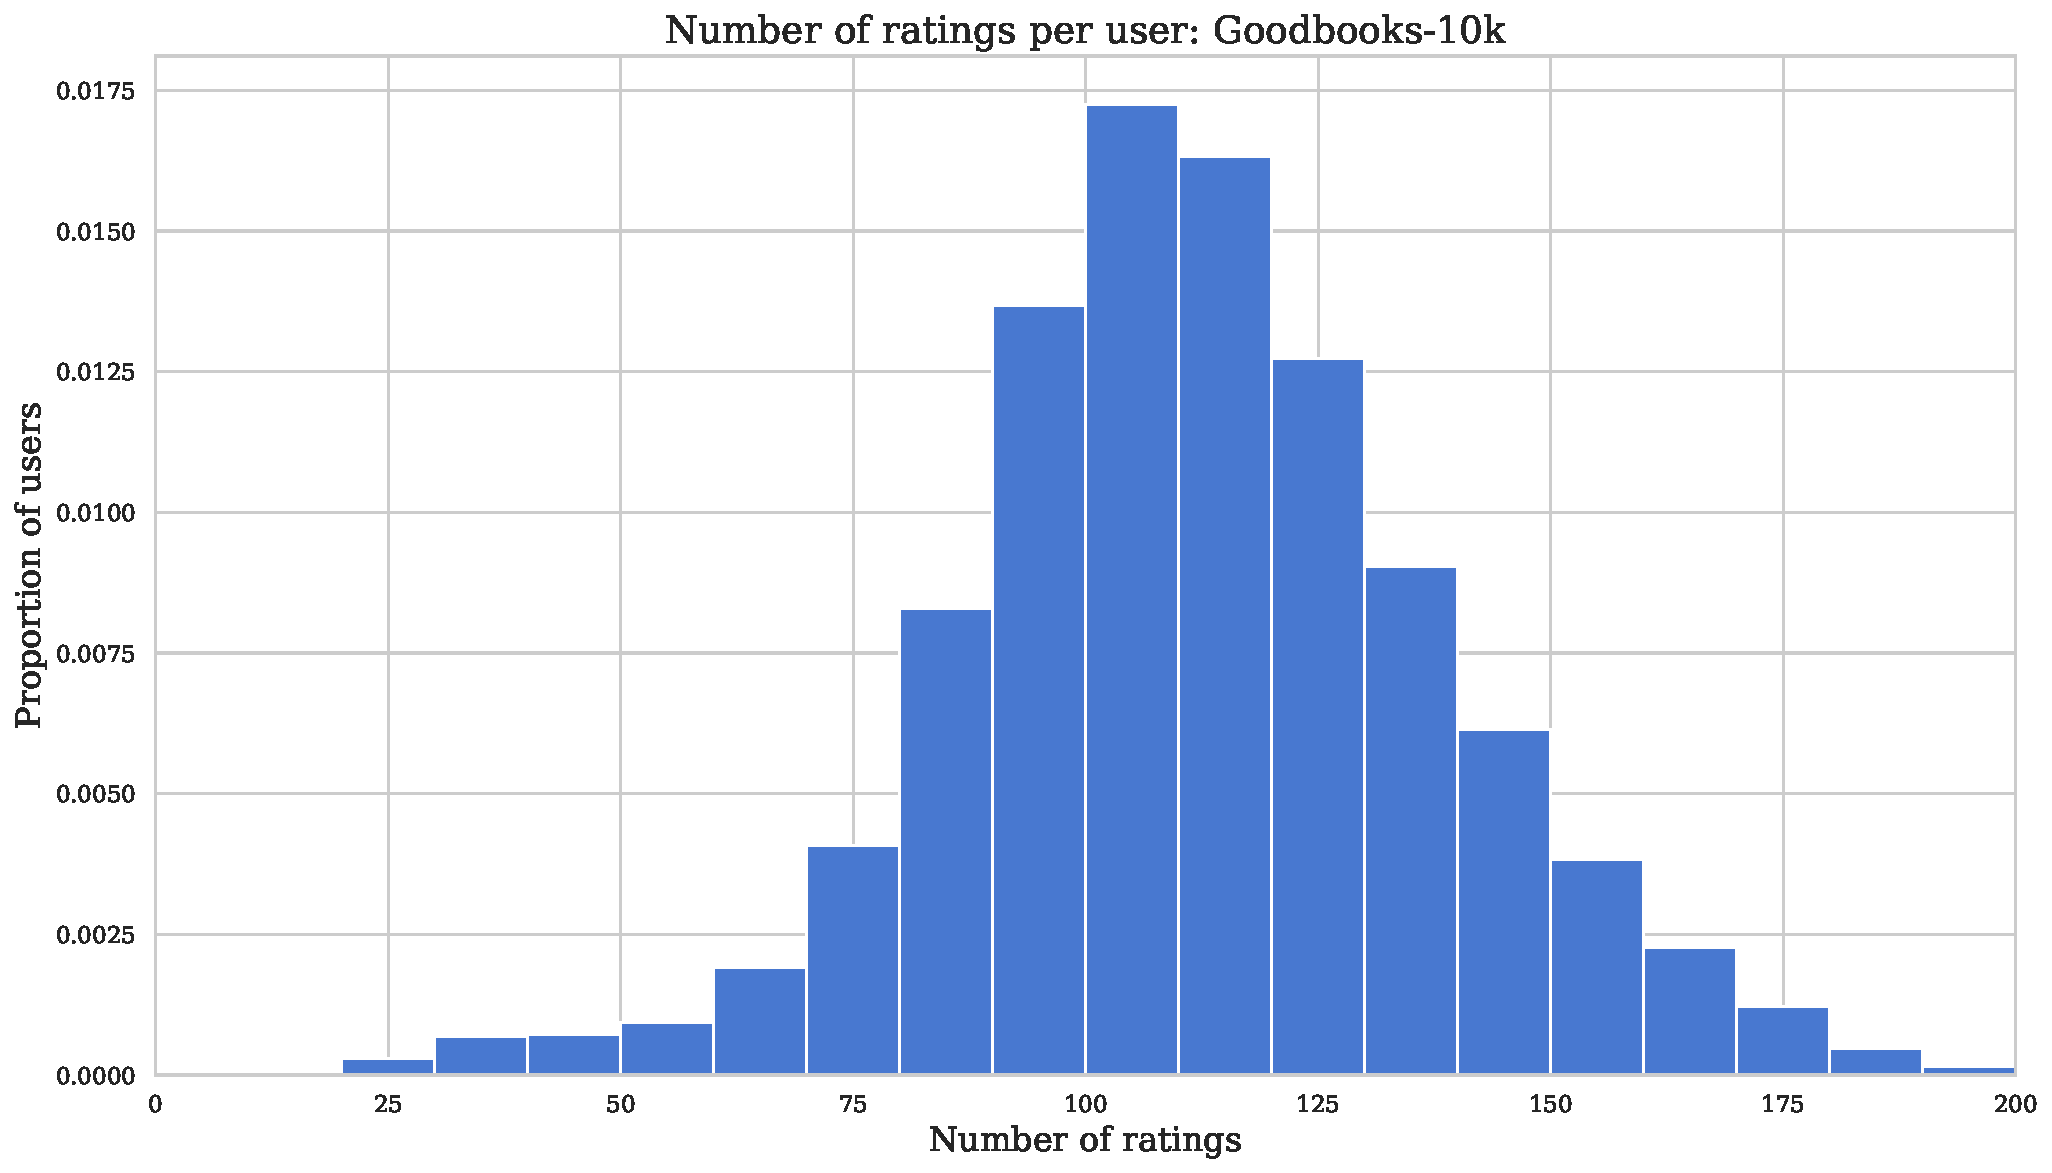
\includegraphics[width=0.75\textwidth]{Figures/3_ratings-distributions/goodbooks_user-ratings.pdf}
\caption{Goodbooks-10k number of ratings per user. Number of ratings per user is roughly normally distributed.}
\label{fig:goodbooks-users}
\end{figure}

\subsection{Number of Ratings per Item}
The number of ratings per movie in the MovieLens datasets follow a similar right-tailed distribution to the number of ratings per user; however, since there are fewer movies than users, the average number of ratings per movie is higher.

The number of ratings per book in the Goodbooks-10k dataset does not follow a symmetric distribution, as is the case with ratings per user. Instead, the number of ratings per book in this dataset follows a similar right-tailed pattern to the MovieLens datasets.

Figures \ref{fig:ML10M-items} and \ref{fig:goodbooks-items} show the distributions of the number of ratings per item in the ML 10M and Goodbooks-10k datasets respectively. As is the case with the distributions of the number of ratings per user, the three MovieLens datasets all have similar distributions across number of ratings per item and so only the largest of the datasets is shown below.

\begin{figure}[H]
\centering
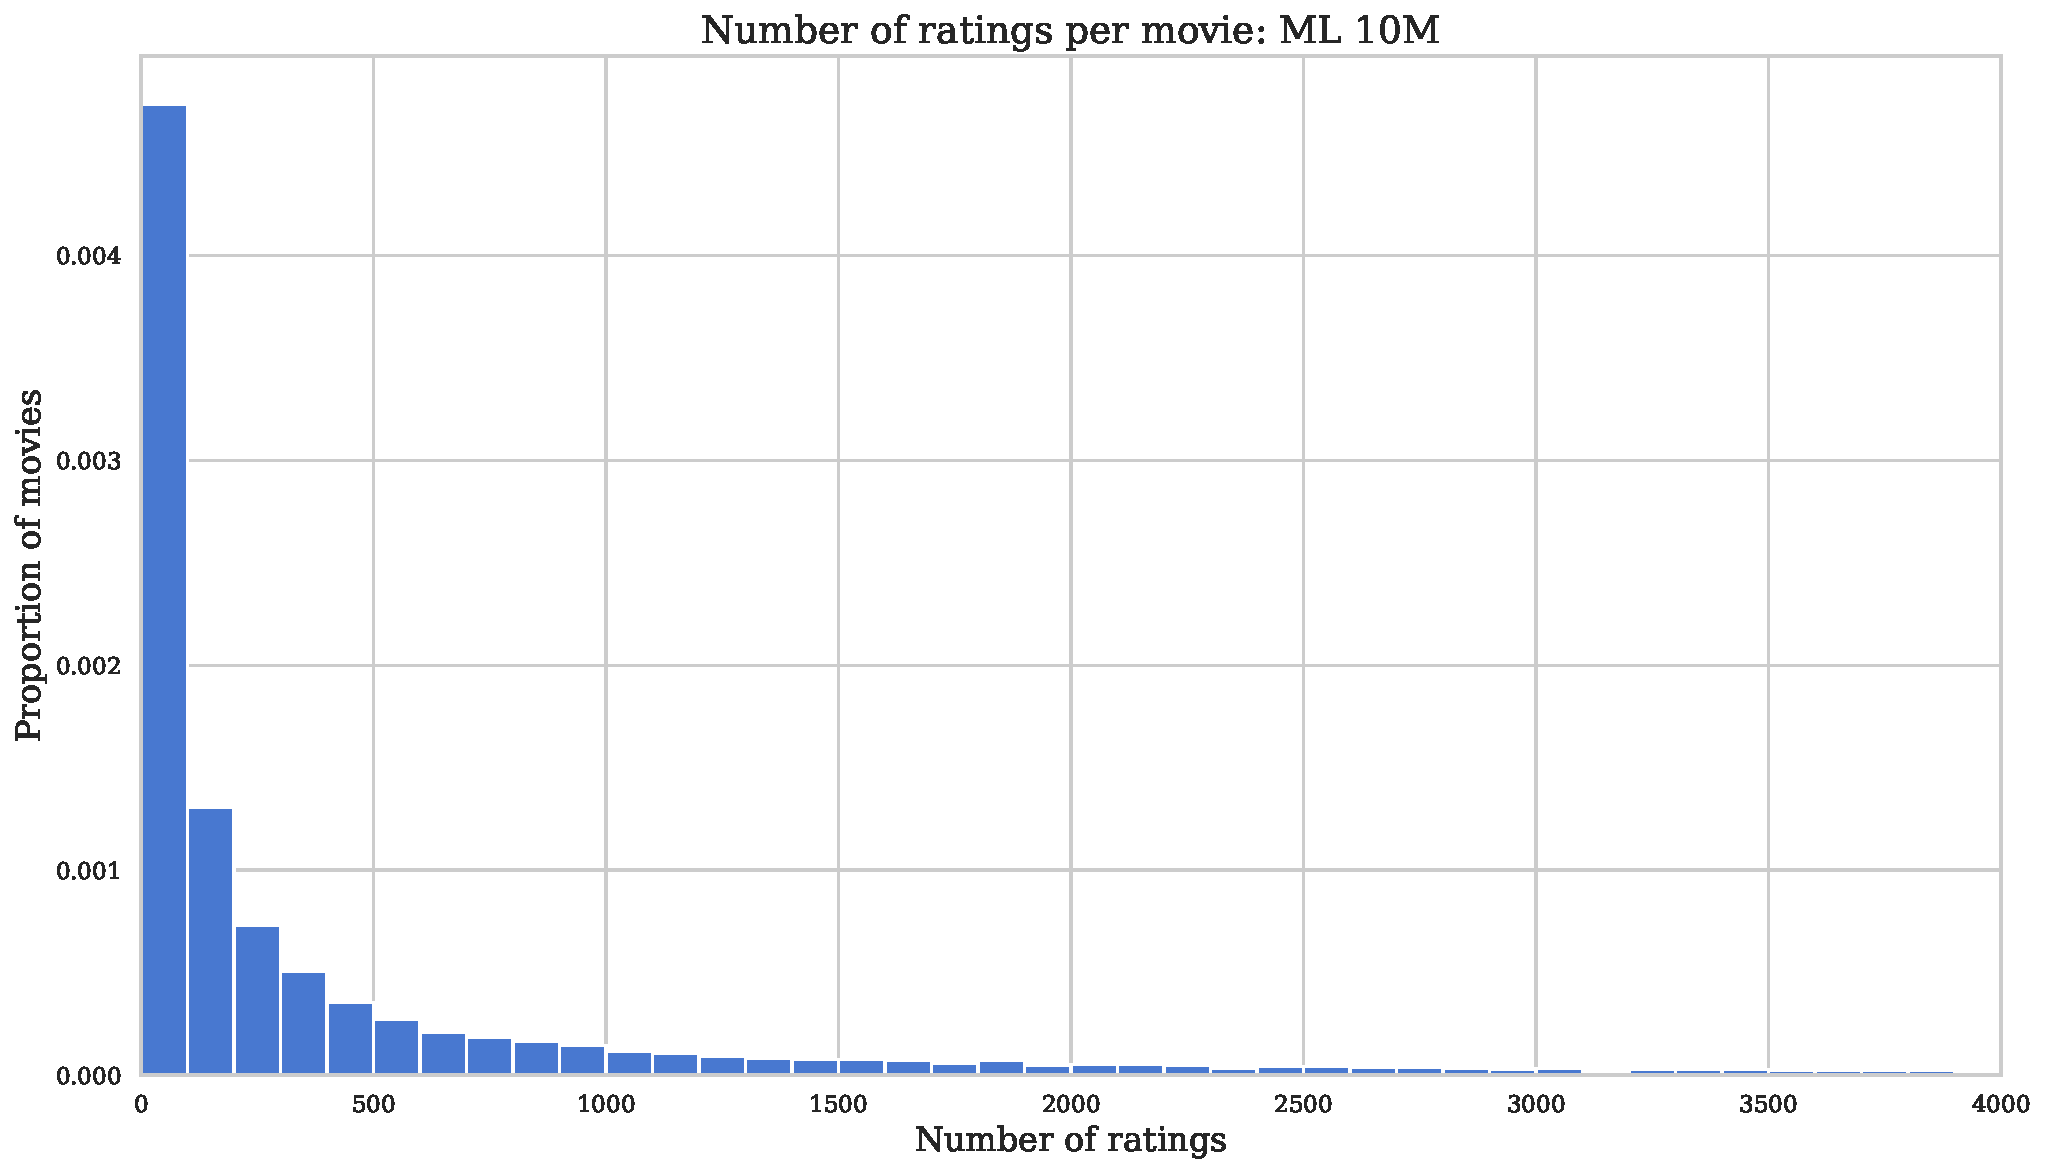
\includegraphics[width=0.75\textwidth]{Figures/3_ratings-distributions/ml_10m_movie-ratings.pdf}
\caption{ML 10M number of ratings per movie.}
\label{fig:ML10M-items}
\end{figure}

\begin{figure}[H]
\centering
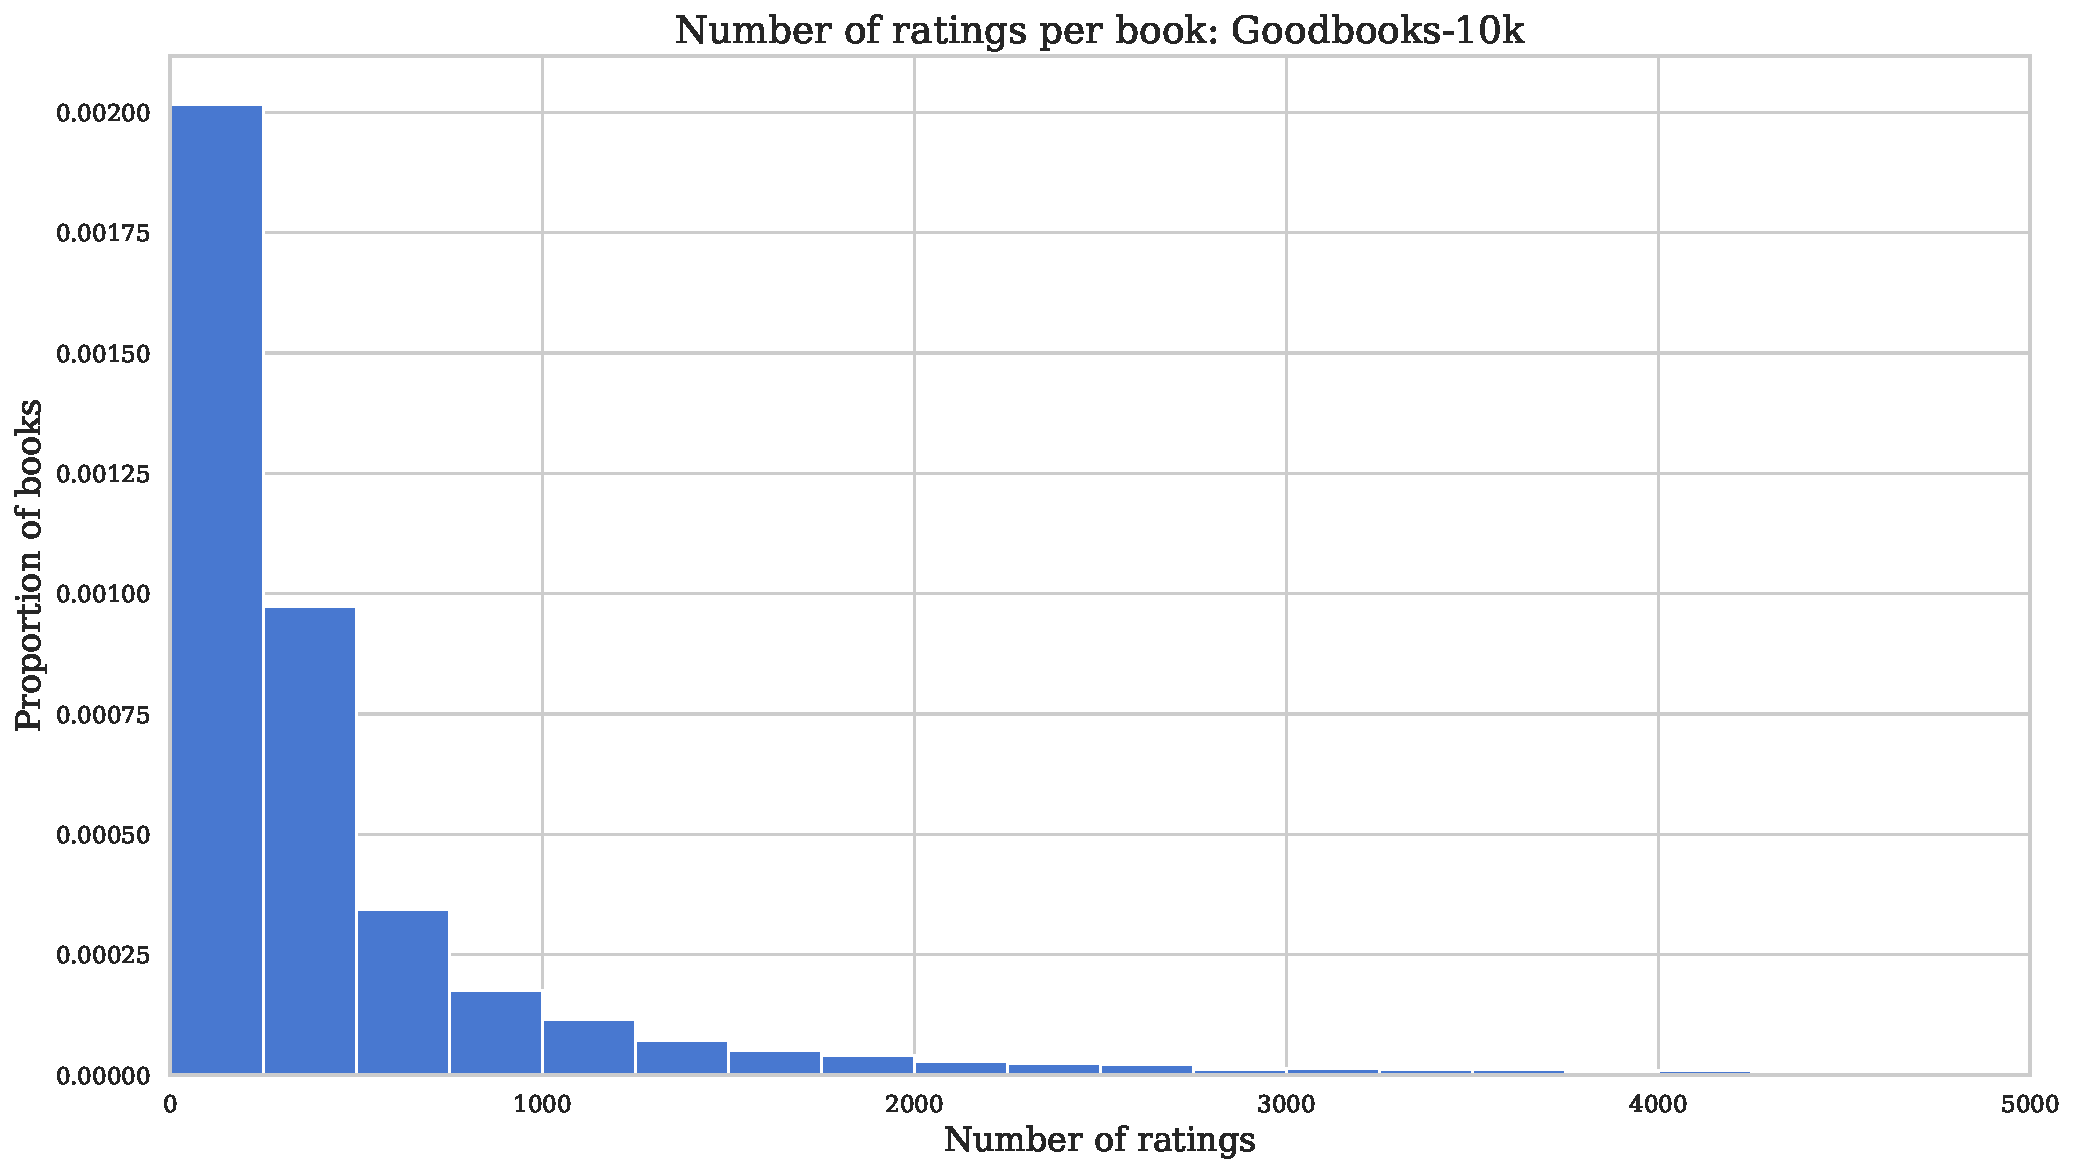
\includegraphics[width=0.75\textwidth]{Figures/3_ratings-distributions/goodbooks-ratings.pdf}
\caption{Goodbooks-10k number of ratings per book.}
\label{fig:goodbooks-items}
\end{figure}

\subsection{Rating Scales}
In all of the datasets, the data are skewed in favour of positive ratings. For example, MovieLens 100k uses a 5-point integer-only rating scale. The middle value of this scale is 3 stars out of 5; however, the mean user rating is 3.53 and the median is 4. In each of the four datasets, both the median and mean values are higher than the middle point of the respective rating scale. Table \ref{tab:ratings-5-number-summaries} shows the 5-number summaries of each dataset.

\begin{table}[H]
\centering
\begin{tabular}{c | c | c | c | c | c | c}
\toprule
\textbf{Name} & \textbf{Min rating} & \textbf{Q2} & \textbf{Median} & \textbf{Q4} & \textbf{Max rating} & \textbf{Mean rating} \\
\midrule
ML 100K & 1 & 3 & 4 & 4 & 5 & 3.53 \\
ML 1M & 1 & 3 & 4 & 4 & 5 & 3.58 \\
ML 10M & 0.5 & 3.0 & 4.0 & 4.0 & 5.0 & 3.51 \\
Goodbooks-10k & 1 & 3 & 4 & 5 & 5 & 3.92 \\
\bottomrule
\end{tabular}
\caption[5-number of summaries of ratings]{Summary of the distribution of ratings in each dataset}
\label{tab:ratings-5-number-summaries}
\end{table}

\section{Distribution of Genres}
All MovieLens datasets, as well as Goodbooks-10k, include item meta data. In the case of MovieLens, movies have been tagged with at least one of a total of 18 genres. Books in Goodbooks-10k have been tagged with at least one of 10 genres. Since the items in all four of these datasets may be labelled with one or more genres simultaneously, attempting to predict their genres is considered a multi-label classification problem.

Table \ref{tab:ML-genres} shows the 18 genre categories used in the MovieLens datasets, as well as the proportion of movies that were assigned that genre.

\begin{table}[H]
\centering
\begin{tabular}{c | c | c | c}
\toprule
\textbf{Genre} & \textbf{ML 100k} & \textbf{ML 1M} & \textbf{ML 10M} \\
\midrule
Action & 0.149 & 0.134 & 0.138 \\
Adventure & 0.080 & 0.076 & 0.096 \\
Animation & 0.025 & 0.028 & 0.027 \\
Children's & 0.073 & 0.067 & 0.049 \\
Comedy & 0.300 & 0.314 & 0.350 \\
Crime & 0.065 & 0.054 & 0.105 \\
Documentary & 0.030 & 0.030 & 0.045 \\
Drama & 0.431 & 0.403 & 0.500 \\
Fantasy & 0.013 & 0.018 & 0.051 \\
Film-Noir & 0.014 & 0.012 & 0.014 \\
Horror & 0.054 & 0.091 & 0.095 \\
Musical & 0.033 & 0.030 & 0.041 \\
Mystery & 0.036 & 0.028 & 0.048 \\
Romance & 0.147 & 0.124 & 0.158 \\
Sci-Fi & 0.060 & 0.074 & 0.071 \\
Thriller & 0.149 & 0.131 & 0.160 \\
War & 0.042 & 0.038 & 0.048 \\
Western & 0.016 & 0.018 & 0.026 \\
\bottomrule
\end{tabular}
\caption[Movies per genre as a proportion of the total]{Summary of the distribution of ratings in each dataset}
\label{tab:ML-genres}
\end{table}

From table \ref{tab:ML-genres}, one can see that genre is highly unbalanced. Of all the categories, drama has the greatest representation, with half of the movies in ML10M falling under this genre. The second most well-represented category is that of comedy, with 35\% of the movies in ML10M falling under this genre.
\chapter{Methodology}
This chapter details the methods used in this dissertation. Specifically, the focus is on collaborative genre tagging (CGT) - a sequential transfer learning approach that applies collaborative filtering to predict genres of items such as movies or books. First, CGT is outlined and compared to more common uses of collaborative filtering on datasets such as MovieLens and Goodbooks. Then, the model architecture of CGT is detailed, along with the key hyperparameters to be tuned. Finally, the framework for hyperparameter tuning and model evaluation is described.

\section{Collaborative genre tagging}
Most of the previous work on collaborative filtering (CF) tackled the problem of predicting user preferences using their interaction history. The most successful methods all involve the use of latent factor models which are capable of learning otherwise hidden properties in the users and items in CF datasets. Recently this type of approach has been adapted from matrix factorisation models to neural architectures which capture latent factors in embedding layers, while allowing for non-linearity in fully connected hidden layers.

The general idea behind CF is that users with similar preferences will provide similar ratings for a given movie. The idea behind CGT is that similar movies will be rated similarly by users who share a preference for that type of movie. This concept is illustrated in figure \ref{fig:4_CGT-concept}. Just as user ratings patterns have been used to infer user preferences, they can also be used to infer information about the items being rated by users.

\begin{figure}[H]
\centering
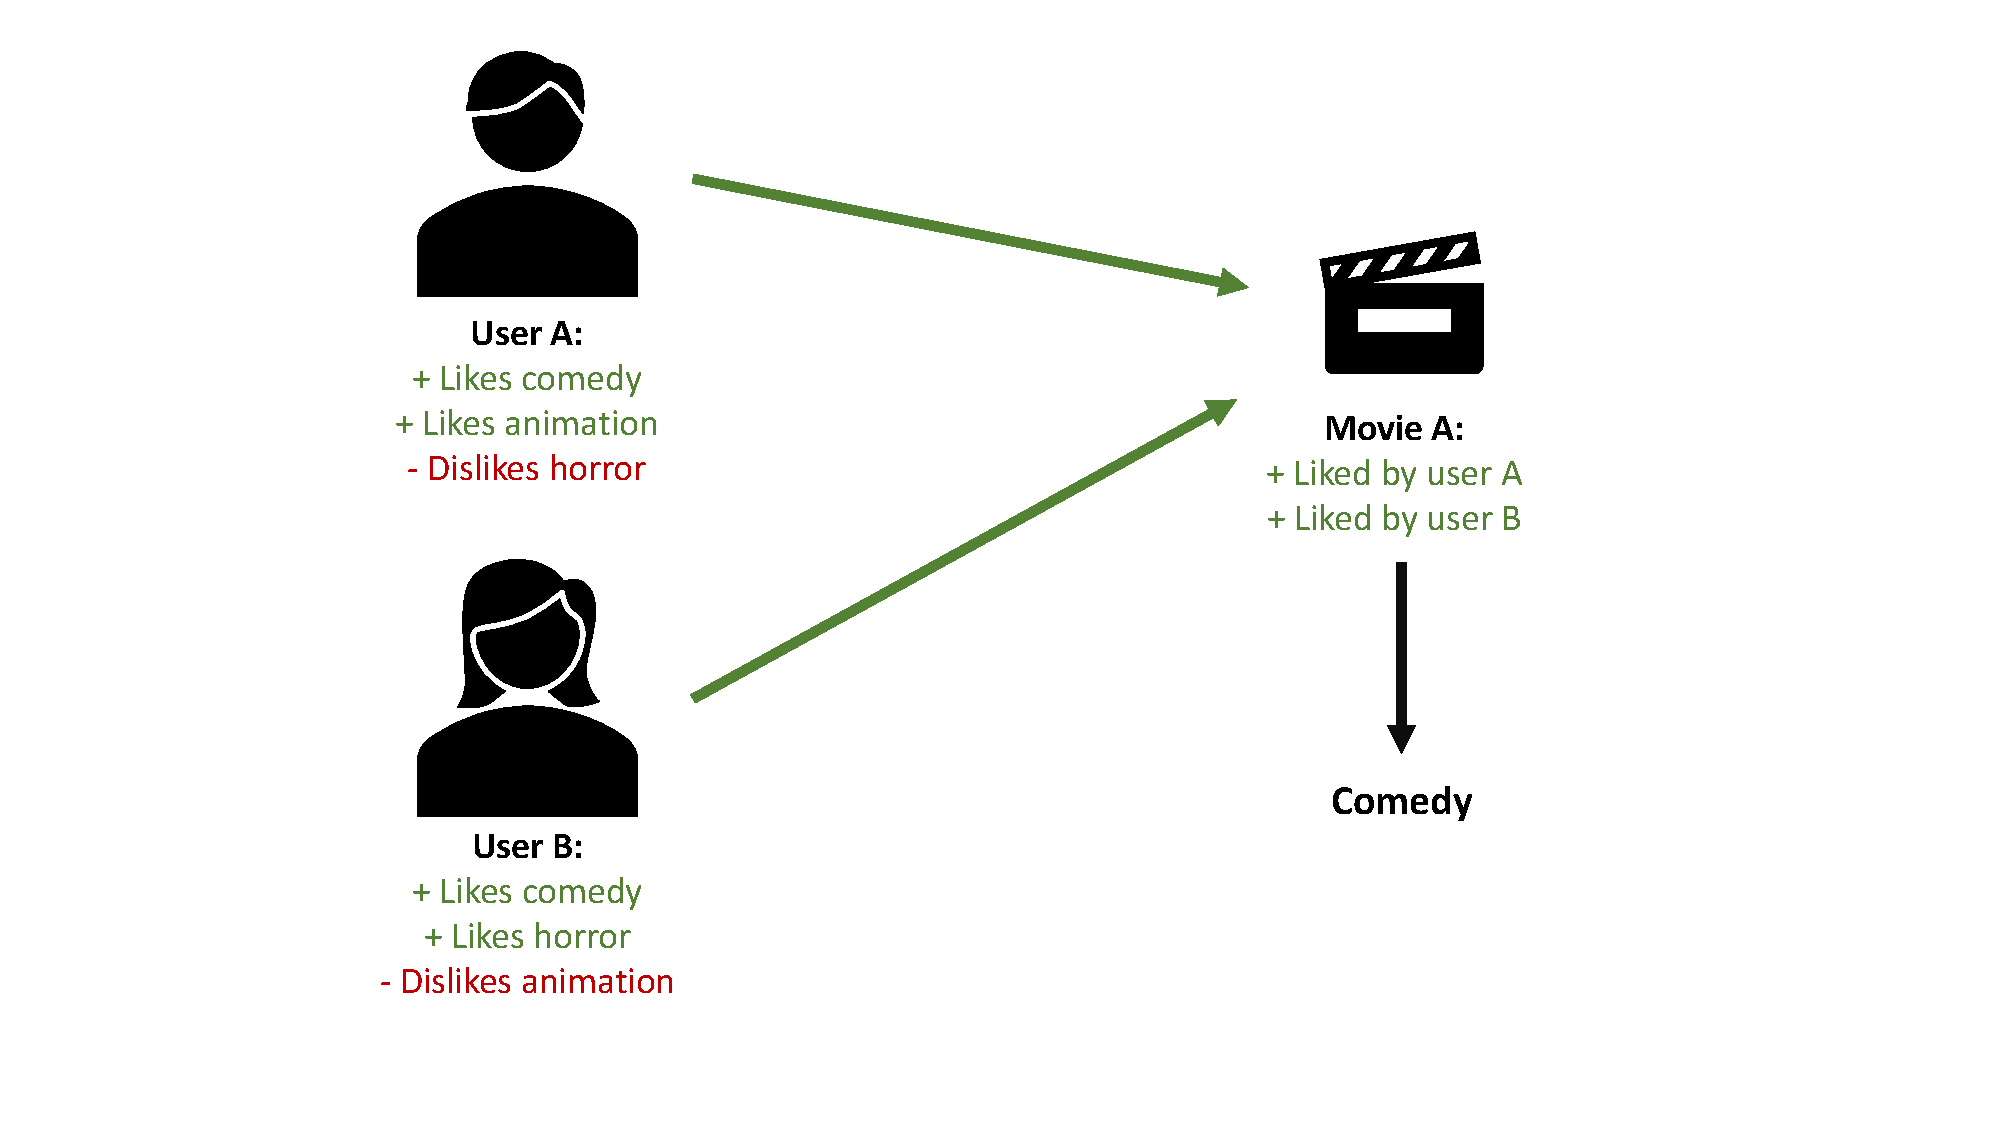
\includegraphics[width=0.85\textwidth]{Figures/4_CGT-concept.pdf}
\decoRule
\caption[Collaborative genre tagging concept]{CGT uses patterns in user ratings to predict genres.}
\label{fig:4_CGT-concept}
\end{figure}

CGT involves two distinct learning tasks, which are:
\begin{enumerate}
    \item learn user and item latent factors through the task of predicting user-item ratings, and
    \item learn to decode item latent factors to genres.
\end{enumerate}
The neural architectures associated with each of the tasks listed above are shown in figure \ref{fig:4_CGT-architecture}. The first model uses latent factors to predict user ratings and is similar in design to the Neural Collaborative Filtering model used by \citeauthor{he2017neural} (the architecture of which is shown in figure \ref{fig:ncf-arch}). The purpose of this model is to train the embedding layer to produce latent factors associated with every item in the ratings dataset.

\begin{figure}[H]
\centering
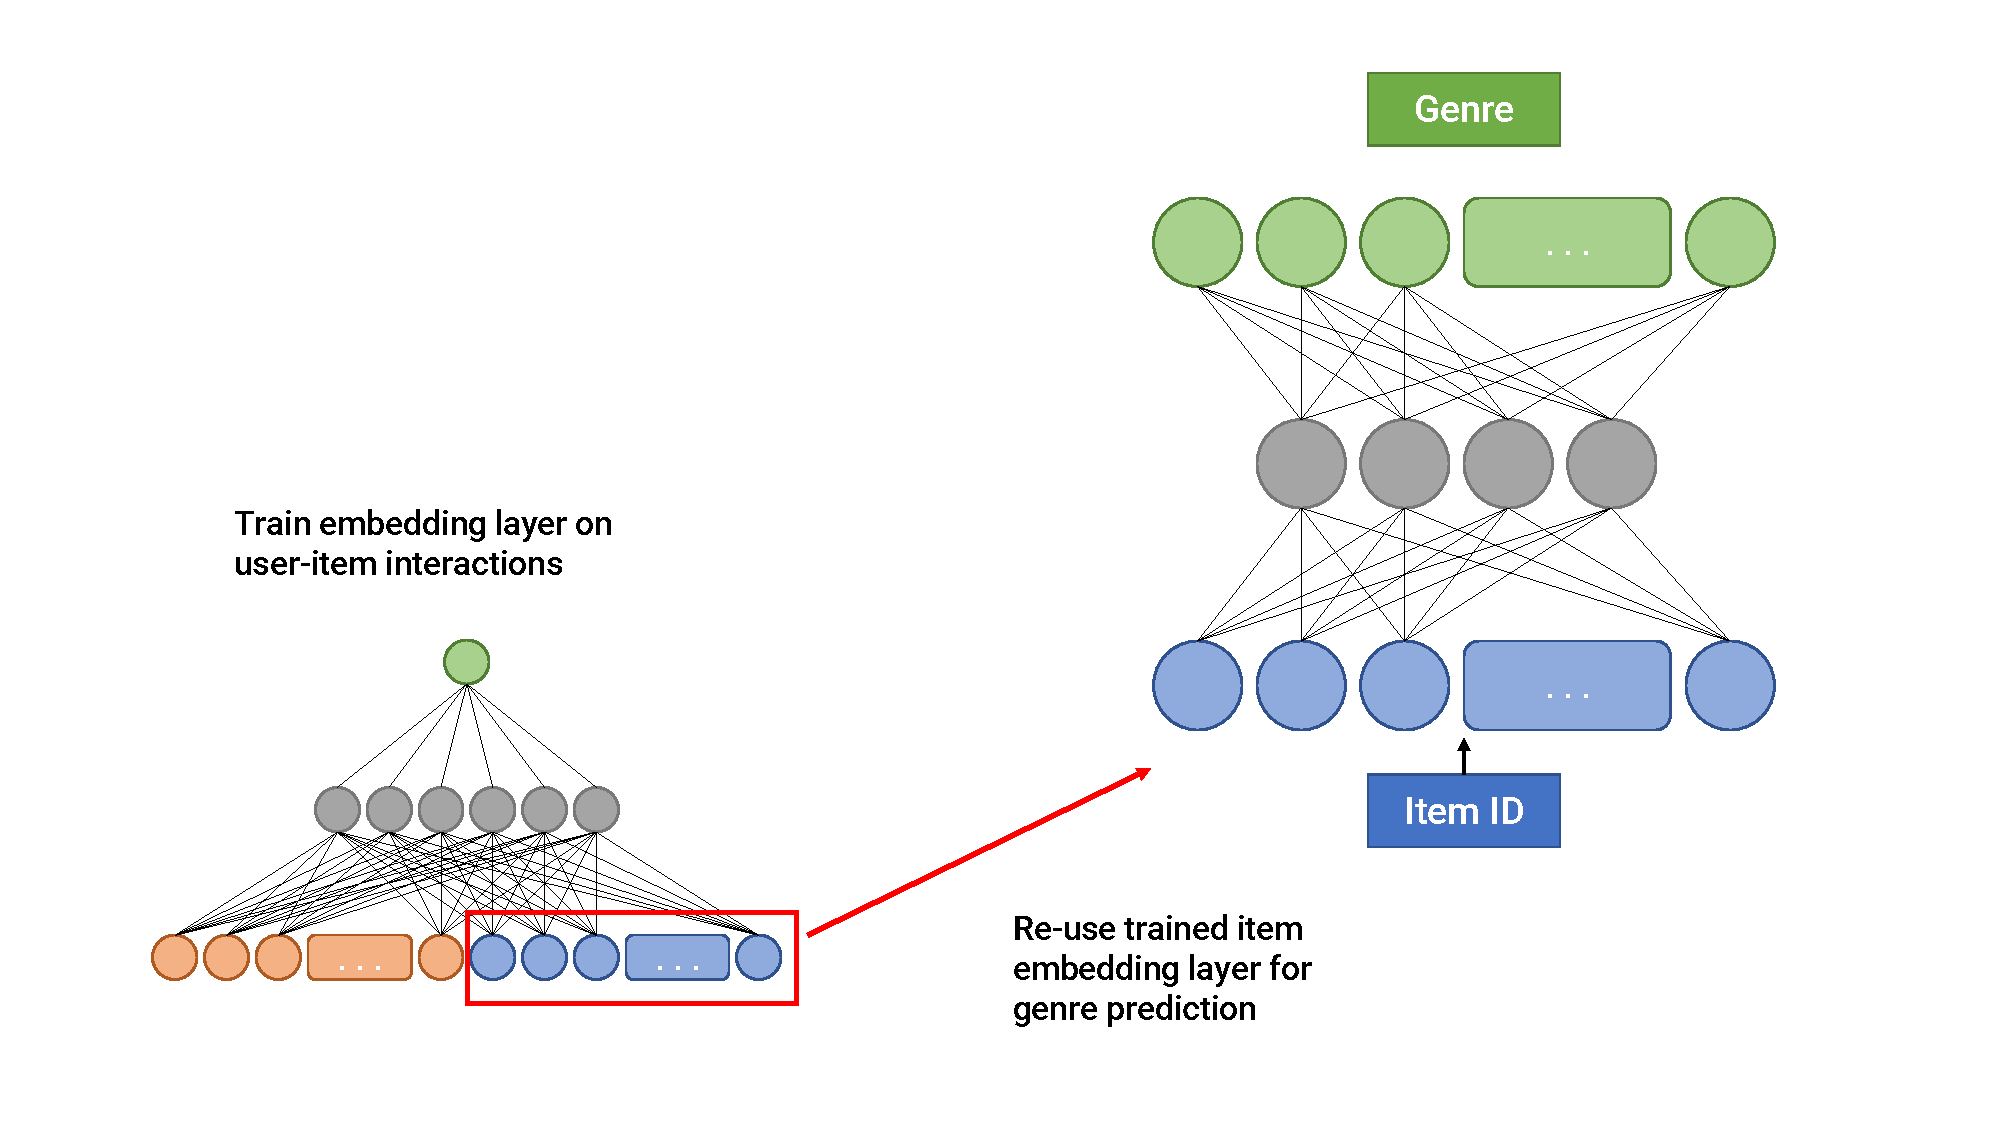
\includegraphics[width=0.9\textwidth]{Figures/4_CGT-model.pdf}
\decoRule
\caption[CGT architecture]{CGT model consists of two neural networks which share a common item embedding layer}
\label{fig:4_CGT-architecture}
\end{figure}

The second model uses the embedding layer of the first, with a hidden layer used to decode item latent factors to genres. The models are trained sequentially, with the shared embedding layer being frozen when training the second model.

\section{Rating model}
\label{section:rating-model}
The rating model is the base of the CGT model. The input to this model is a user-item ID pair, and the output is an explicit rating. The IDs in the input pair are connected to an embedding layer of $k\times2$ length, where $k$ is the number of latent factors for both users and items. The embedding layer then feeds to a fully connected layer and then finally into a single output node which contains the predicted rating.

\begin{figure}[H]
\centering
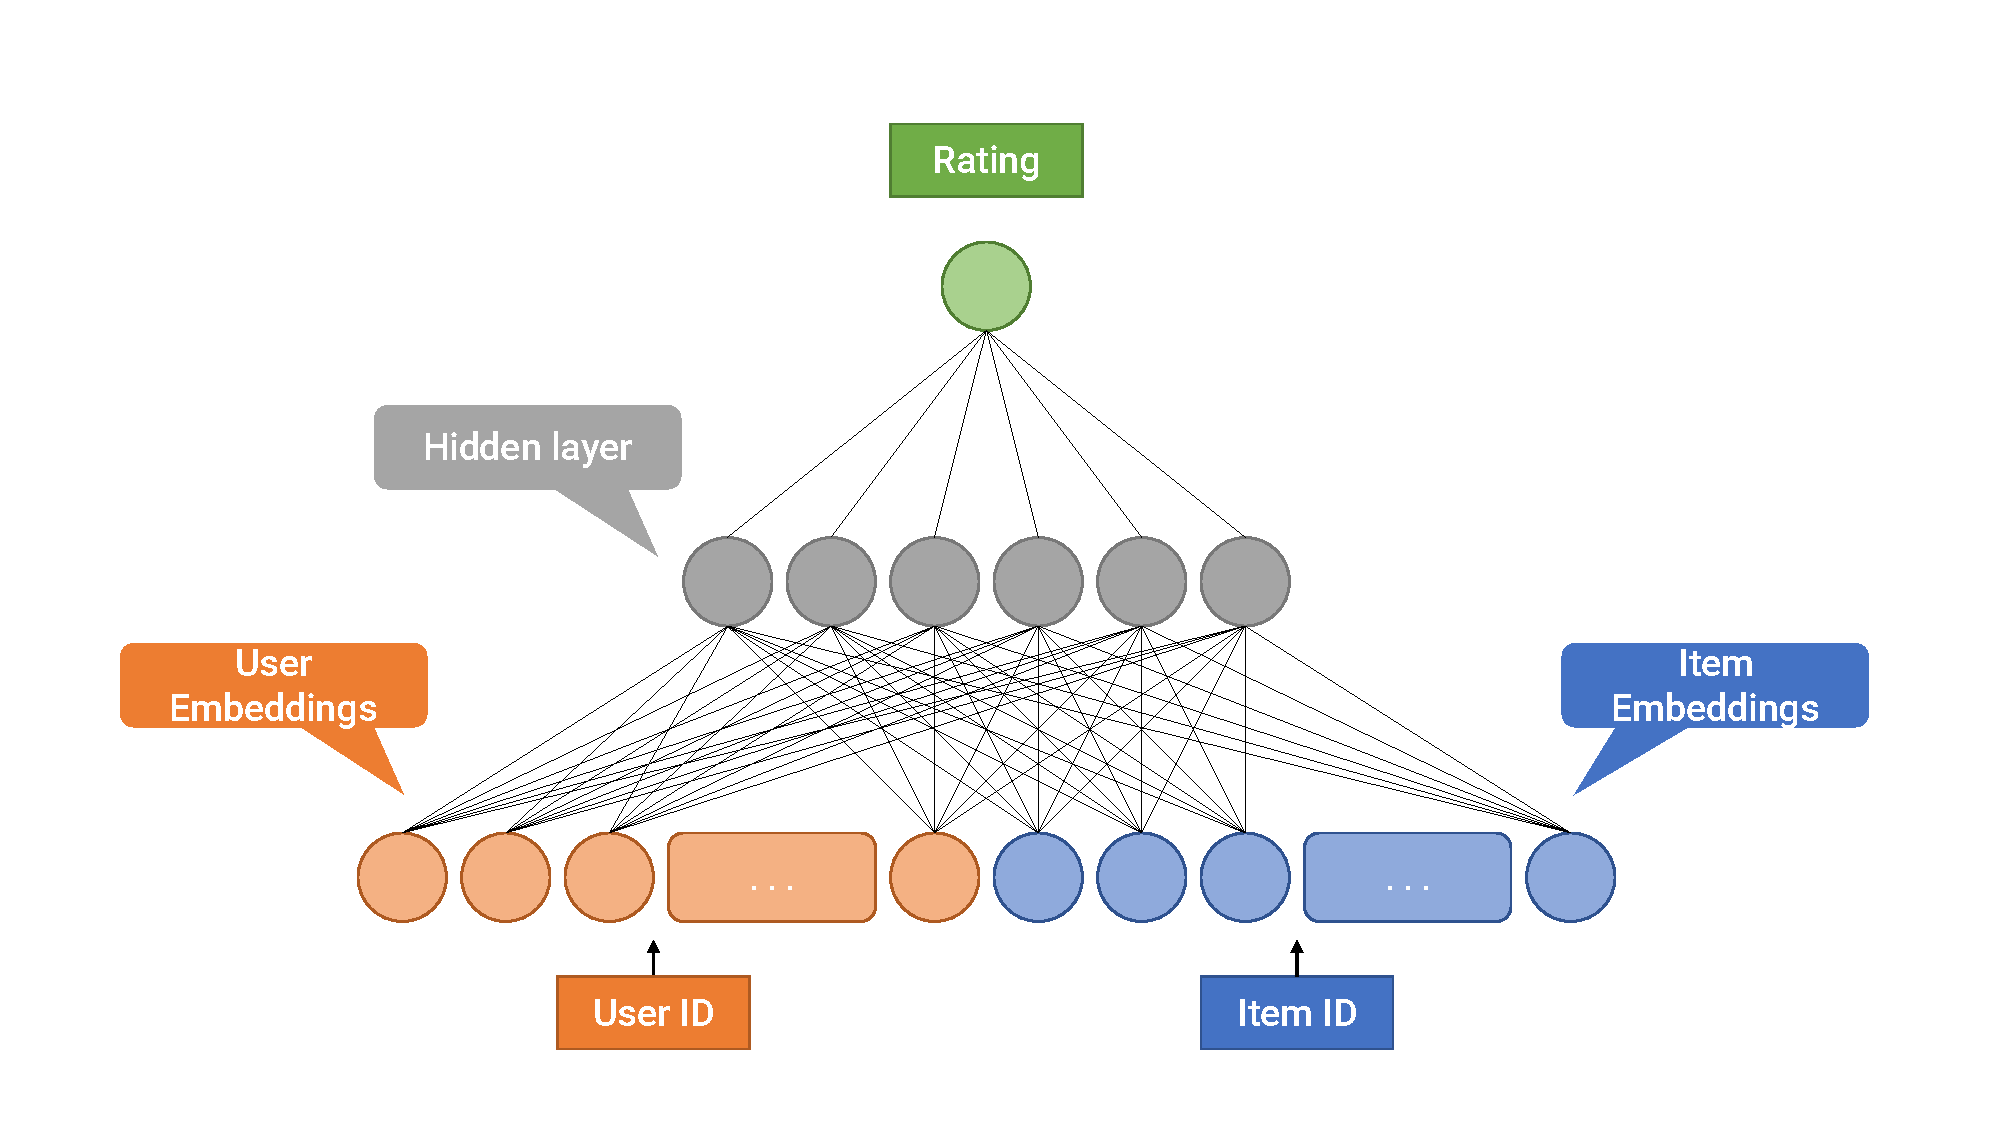
\includegraphics[width=0.85\textwidth]{Figures/4_rating-model.pdf}
\decoRule
\caption[Rating model]{Rating model uses embeddings to capture latent factors of items and users}
\label{fig:4_rating-prediction-architecture}
\end{figure}

\subsection{Embedding layer}
The first layer of the rating model is a concatenated embedding layer. This layer is comprised of two separate embedding matrices, the same as those used in the matrix factorisation method popularised by \citeauthor{koren2009matrix}. These embedding matrices hold the latent factors of all users and items respectively. The user matrix is of dimension $m\times k$ while the item matrix is $n\times k$, where $m$ and $n$ are the number of distinct users and items respectively, and $k$ is the number of latent factors. Figure \ref{fig:4_CGT-embedding-layer} illustrates the combination of latent factor matrices to form the concatenated embedding layer.

\begin{figure}[H]
\centering
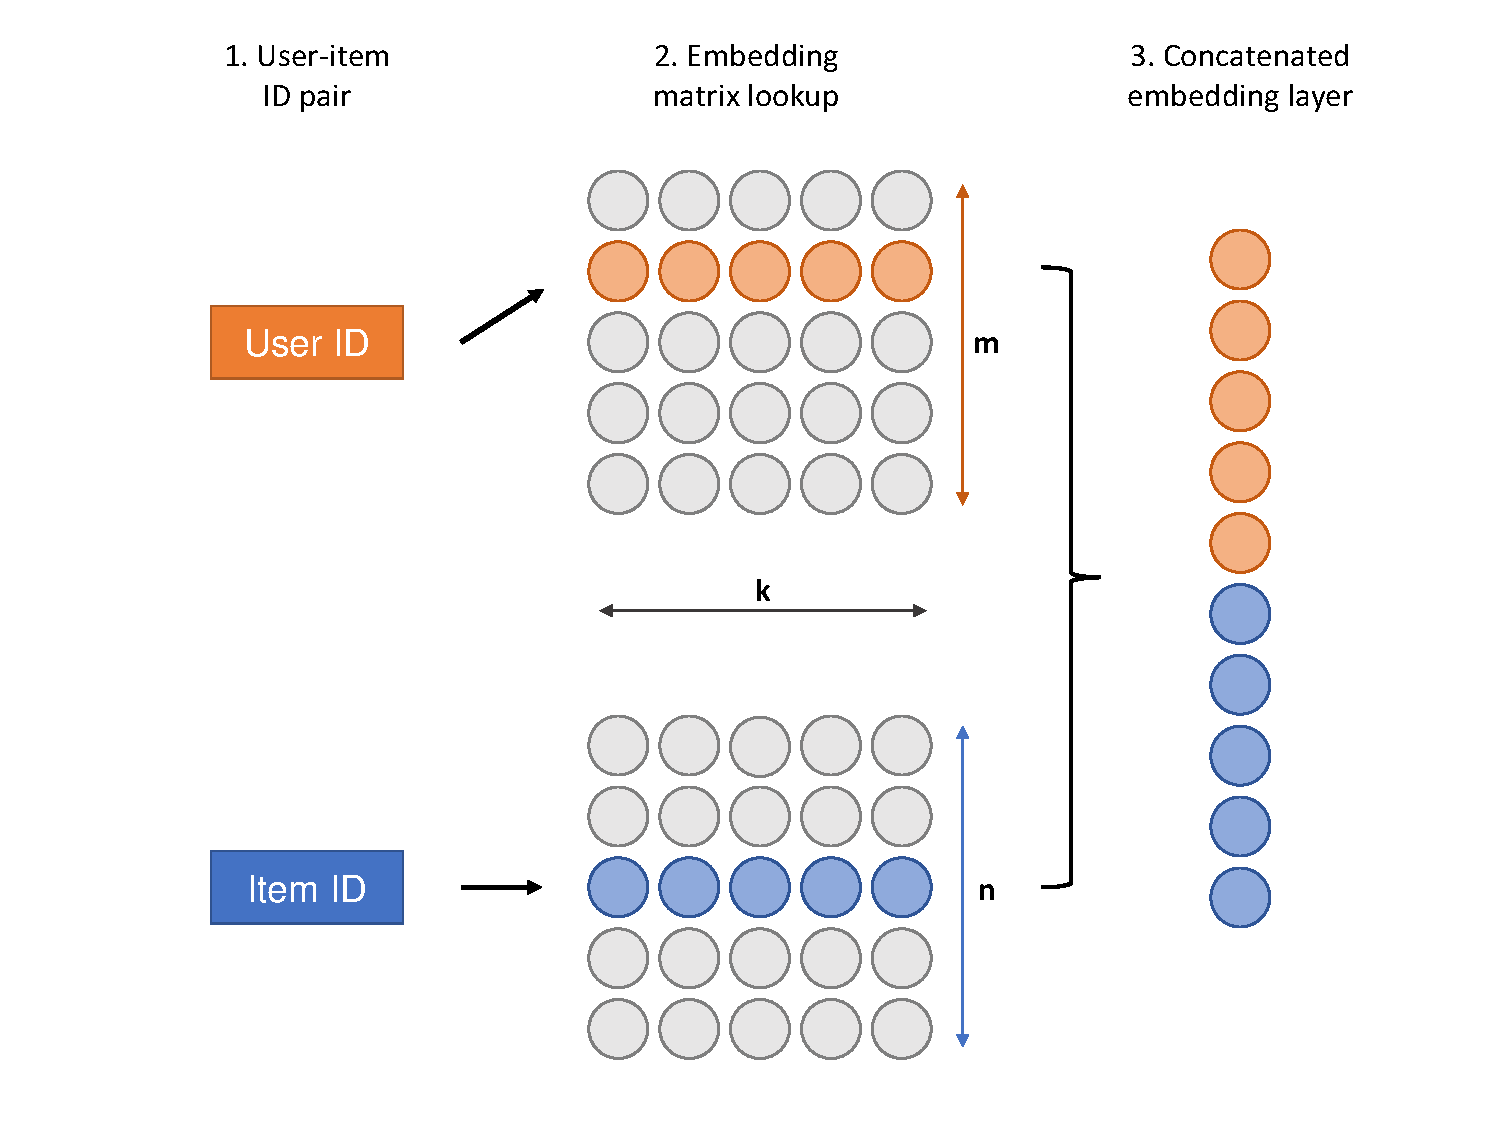
\includegraphics[width=0.8\textwidth]{Figures/4_CGT-embedding-layer.pdf}
\decoRule
\caption[Embedding layer]{Embedding layer is created as the concatenation of two separate embedding matrix lookups.}
\label{fig:4_CGT-embedding-layer}
\end{figure}

The embedding layer is the input layer of the model, which takes a user-item ID pair as its input. Each of these IDs is passed to its respective embedding matrix (step 2 in figure \ref{fig:4_CGT-embedding-layer}) as a lookup to obtain two $k$-dimensional latent factor vectors. These two latent factor vectors are then concatenated together to form the first layer of the neural network. Since each latent factor vector is of length $k$, the concatenated first layer is of dimension $k\times2$. The size of $k$ is a hyperparameter which will need to be tuned.

\subsection{Hidden layer}
The concatenated embedding layer feeds forward into the fully connected hidden layer of the model with $h$ nodes. This hidden layer allows for the model to learn non-linear patterns in the concatenated latent factor vector through the addition of activation functions. It is this non-linearity in the hidden layer that distinguishes the CGT rating model from vanilla matrix factorisation. During training of the model, dropout may also be added to this layer as a means of regularization. The number of nodes in this layer, the choice of activation function and the dropout rate are all hyperparameters that will need to be tuned. Figure \ref{fig:4_CGT-hidden-layer} shows the overall architecture of the rating model.

\begin{figure}[H]
\centering
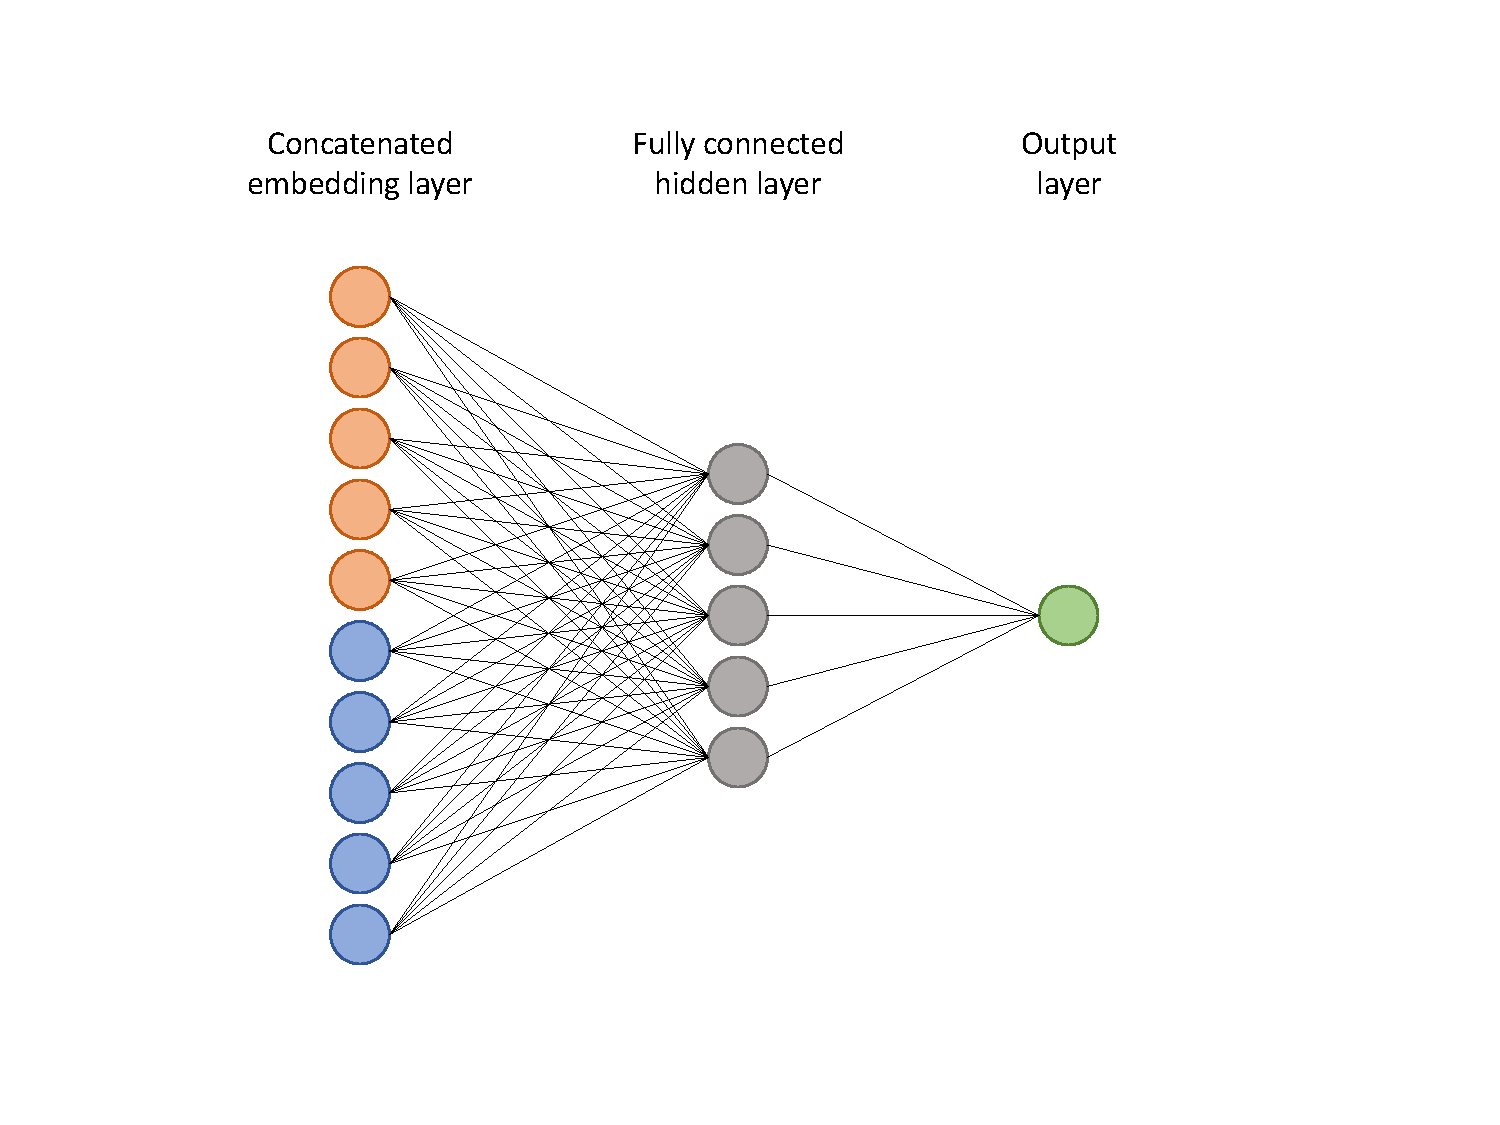
\includegraphics[width=0.8\textwidth]{Figures/4_CGT-hidden.pdf}
\decoRule
\caption[Rating model hidden layer]{Hidden layer is fully connected to concatenated embedding layer and feeds into the output node.}
\label{fig:4_CGT-hidden-layer}
\end{figure}

\subsection{Output layer}
As discussed in section \ref{section:rating-model}, the model takes two inputs: a user and an item ID. The output of the model is a predicted rating of what the input user is expected to rate the input movie. 

The network as it is shown in figure \ref{fig:4_CGT-hidden-layer} does not include any adjustments for user or item biases of any kind. \citeauthor{koren2009matrix} stated that \textit{"much of the observed variation in rating values is due to effects associated with either users or items, known as biases or intercepts, independent of any interactions."} To handle biases inherent in rating data, they adjusted their matrix factorisation model as described in equation \ref{eqn:dot_bias}.

A similar approach has been taken in the CGT model, which adjusts the model output through the addition of the global mean rating, $\mu$, and a specific user-item baseline prediction, $b_{ui}$. This adjustment is illustrated in figure \ref{fig:4_CGT-rating-layer}. 

To calculate the baseline prediction for any user-item combination, one needs to calculate the average biases for both the user and the item. The bias for a user, $b_u$, is calculated as 
\begin{equation}
    b_{u} = \dfrac{\sum_{j=1}^{n_u} (r_{uj} - \mu_i)}{n_u},
\label{eqn:CGT-user-bias}
\end{equation}
which is the average amount by which user $u$'s rating differs from the average rating of an item, $\mu_i$.

Similarly, the bias for an item, $i$, is thus
\begin{equation}
    b_{i} = \dfrac{\sum_{k=1}^{n_i} (r_{ki})}{n_i} - \mu,
\label{eqn:CGT-item-bias}
\end{equation}
which is the difference between the average rating from all users of item $i$ and $\mu$.

Then $b_{ui}$ is calculated as the average between the bias of user $u$ and item $i$, denoted as
\begin{equation}
    b_{ui} = \dfrac{b_u + b_i}{2}.
\label{eqn:CGT-baseline}
\end{equation}

The addition of $b$ and $u$ to the output allows the model to identify the portion the rating that can be identified by biases and subjects only the "true interaction" portion of the data to the embedding and hidden layers. Figure \ref{fig:4_CGT-rating-layer} illustrates the addition baseline predictors to the CGT rating model.

\begin{figure}[H]
\centering
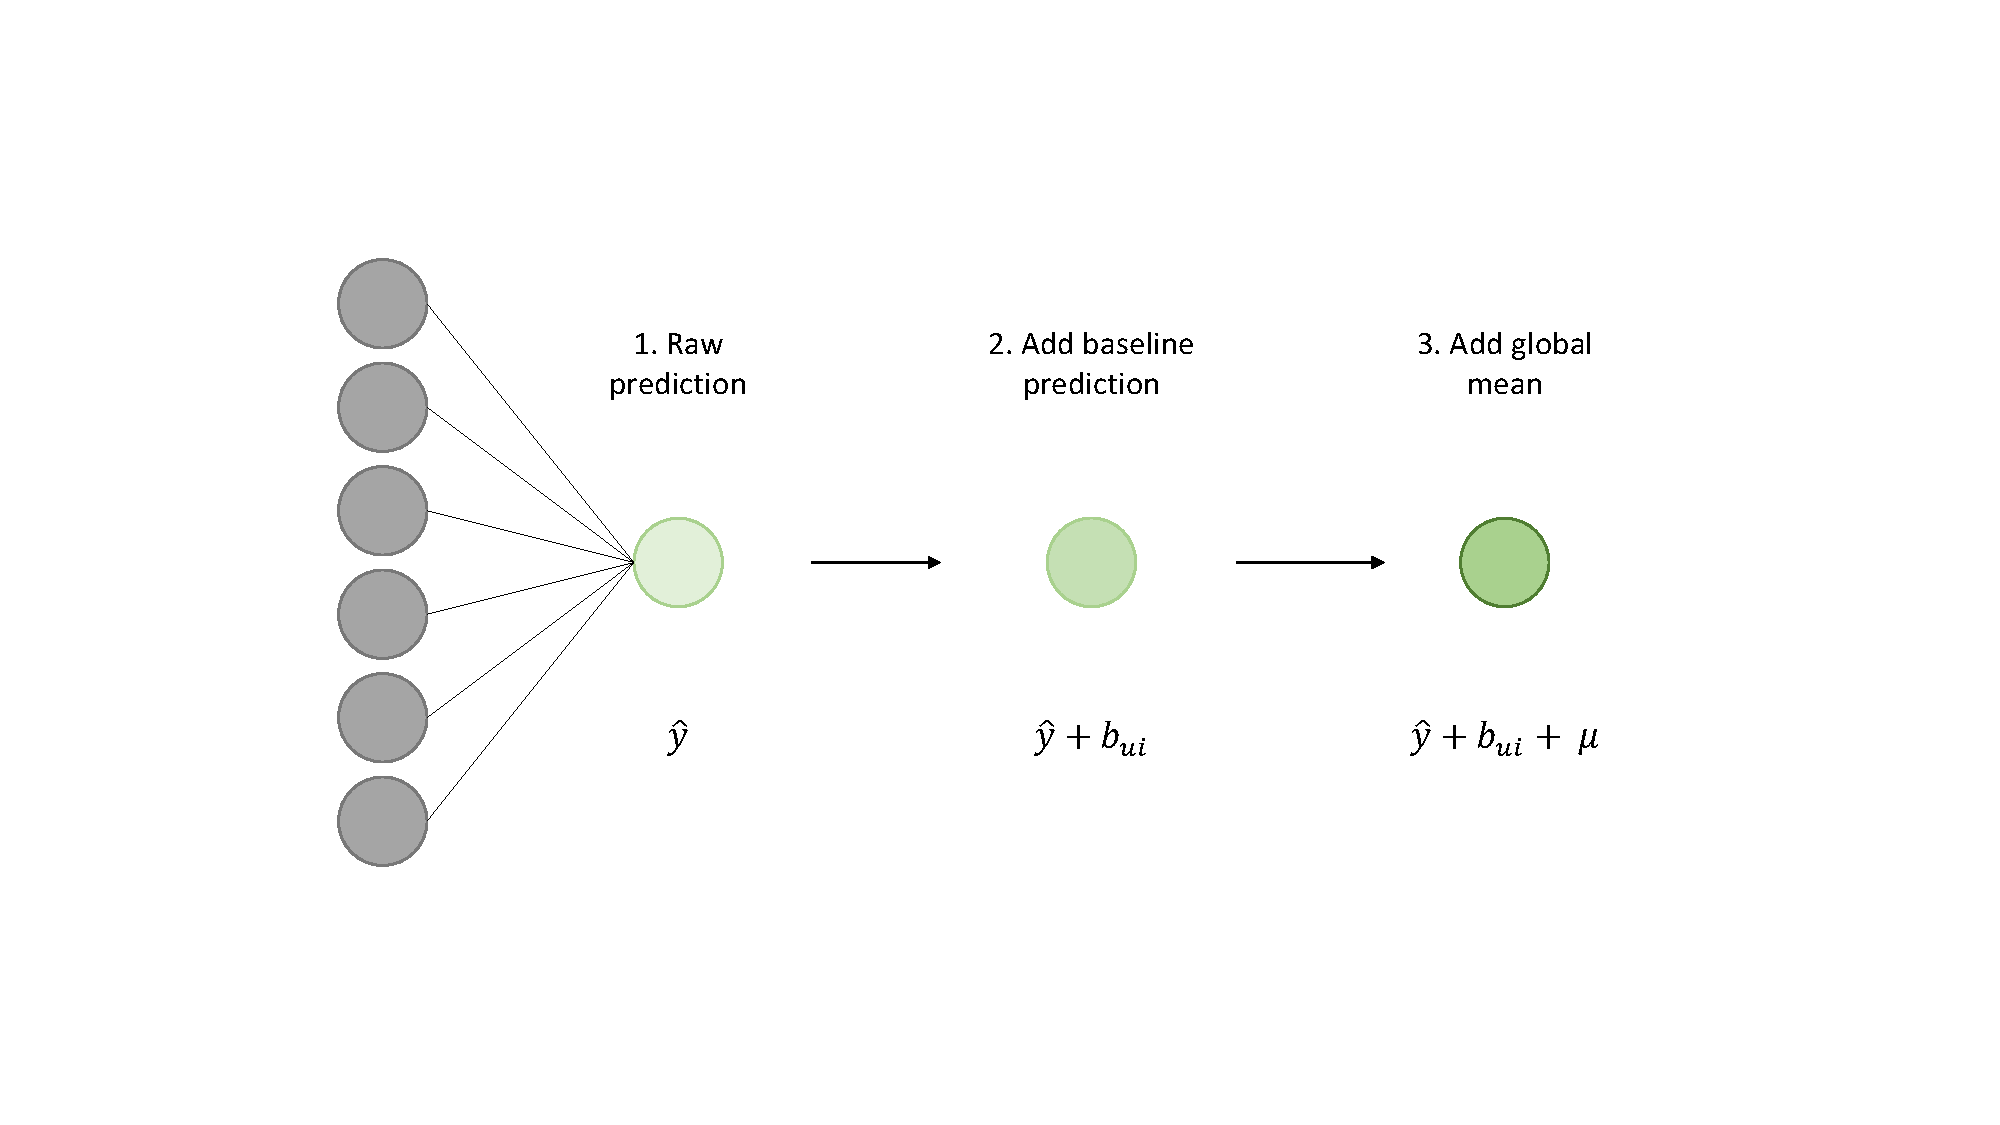
\includegraphics[width=0.9\textwidth]{Figures/4_CGT-output-layer.pdf}
\decoRule
\caption[Rating layer]{Model output is adjusted through the addition of baseline predictors.}
\label{fig:4_CGT-rating-layer}
\end{figure}

The baseline predictors are not learned by the model, they are inherent in the ratings made by users of the system. The values of $b$ and $\mu$ are calculated before training the model using only the ratings from the training set. For any users or items that might appear in a holdout evaluation set but not the training set, the bias is assigned to be $\mu$.

\subsection{Summary of rating model hyperparameters}
Table \ref{tab:rating-hparams} summarises the tunable hyperparameters in the rating model. These hyperparameters were tuned and evaluated with respect to their influence on the accuracy of the final genre prediction.
\begin{table}[H]
\centering
\begin{tabular}{c | p{3.5cm} | c | c}
\toprule
\textbf{Symbol} & \textbf{Description} & \textbf{Type} & \textbf{Range} \\
\midrule
$k$ & Number of latent factors in user and item latent factors & Discrete & (1, $\infty$] \\
\midrule
$h$ & Number of nodes in hidden layer & Discrete & (0, $\infty$] \\
\midrule
$dr1$ & Dropout rate in hidden layer & Continuous & (0, 1) \\
\midrule
$f1$ & Activation function in hidden layer & n/a & n/a \\
\bottomrule
\end{tabular}
\caption[Rating model hyperparameters]{Summary of tunable hyperparameters in CGT rating model, in the case of 0 hidden nodes, the model reproduces matrix factorisation.}
\label{tab:rating-hparams}
\end{table}

\section{Genre model}
The genre model is the second "head" of the CGT model. It re-uses the trained item embedding layer as its input layer and attempts to learn to decode latent factors to genres. The input layer has dimension $k$, following by a hidden layer with $j$ nodes. The output layer has as many nodes as the total number of genres with which the items have been labelled, $g$.

The purpose of this model is to learn how to interpret the latent factors that have been learnt by the first model; it learns to translate the latent feature space into a defined genre label, commonly used by people to describe items.

\begin{figure}[H]
\centering
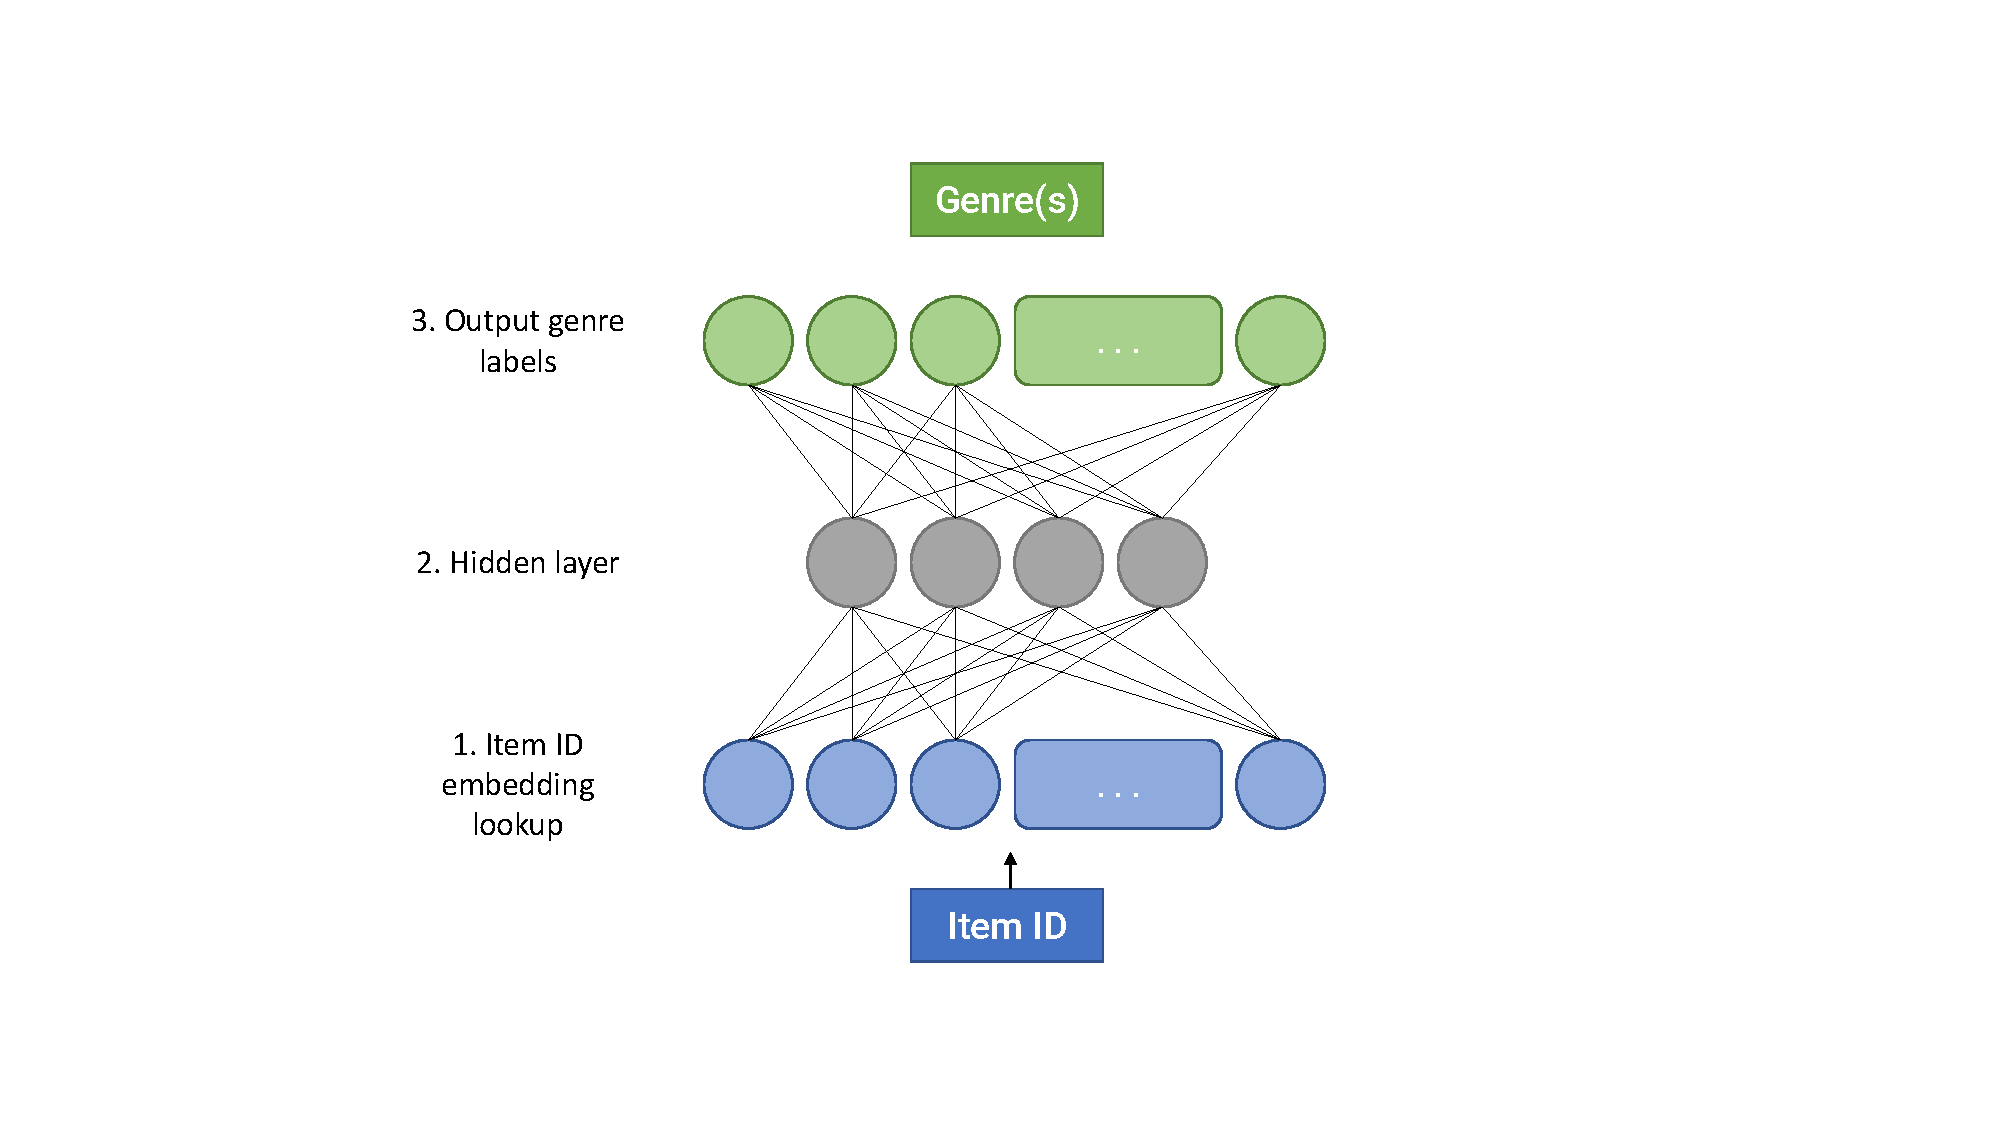
\includegraphics[width=0.75\textwidth]{Figures/4_genre-model.pdf}
\decoRule
\caption[Genre prediction model]{Genre prediction model re-uses the item embedding layer from the base ratings prediction model}
\label{fig:4_genre-prediction-architecture}
\end{figure}

\subsection{Summary of genre model hyperparameters}
\begin{table}[H]
\centering
\begin{tabular}{c | p{3.5cm} | c | c}
\toprule
\textbf{Symbol} & \textbf{Description} & \textbf{Type} & \textbf{Range} \\
\midrule
$j$ & Number of nodes in hidden layer & Discrete & (0, $\infty$] \\
\midrule
$dr2$ & Dropout rate in hidden layer & Continuous & (0, 1) \\
\midrule
$f2$ & Activation function in hidden layer & n/a & n/a \\
\bottomrule
\end{tabular}
\caption[Genre model hyperparameters]{Summary of tunable hyperparameters in CGT genre model.}
\label{tab:genre-hparams}
\end{table}

\section{Tuning and evaluation framework}
The standard approach to hyperparameter tuning of rating models in the past has been to use 5-fold cross validation (CV) on 90\% of the available data, with the remaining 10\% used as a true holdout set for model evaluation. Both the rating and genre model were tuned together, using 5-fold CV on 90\% of the available genre labels, with 10\% used for testing. Figure \ref{fig:4_cross-validation} illustrates the splitting of the dataset for training, validation and testing.

\begin{figure}[H]
\centering
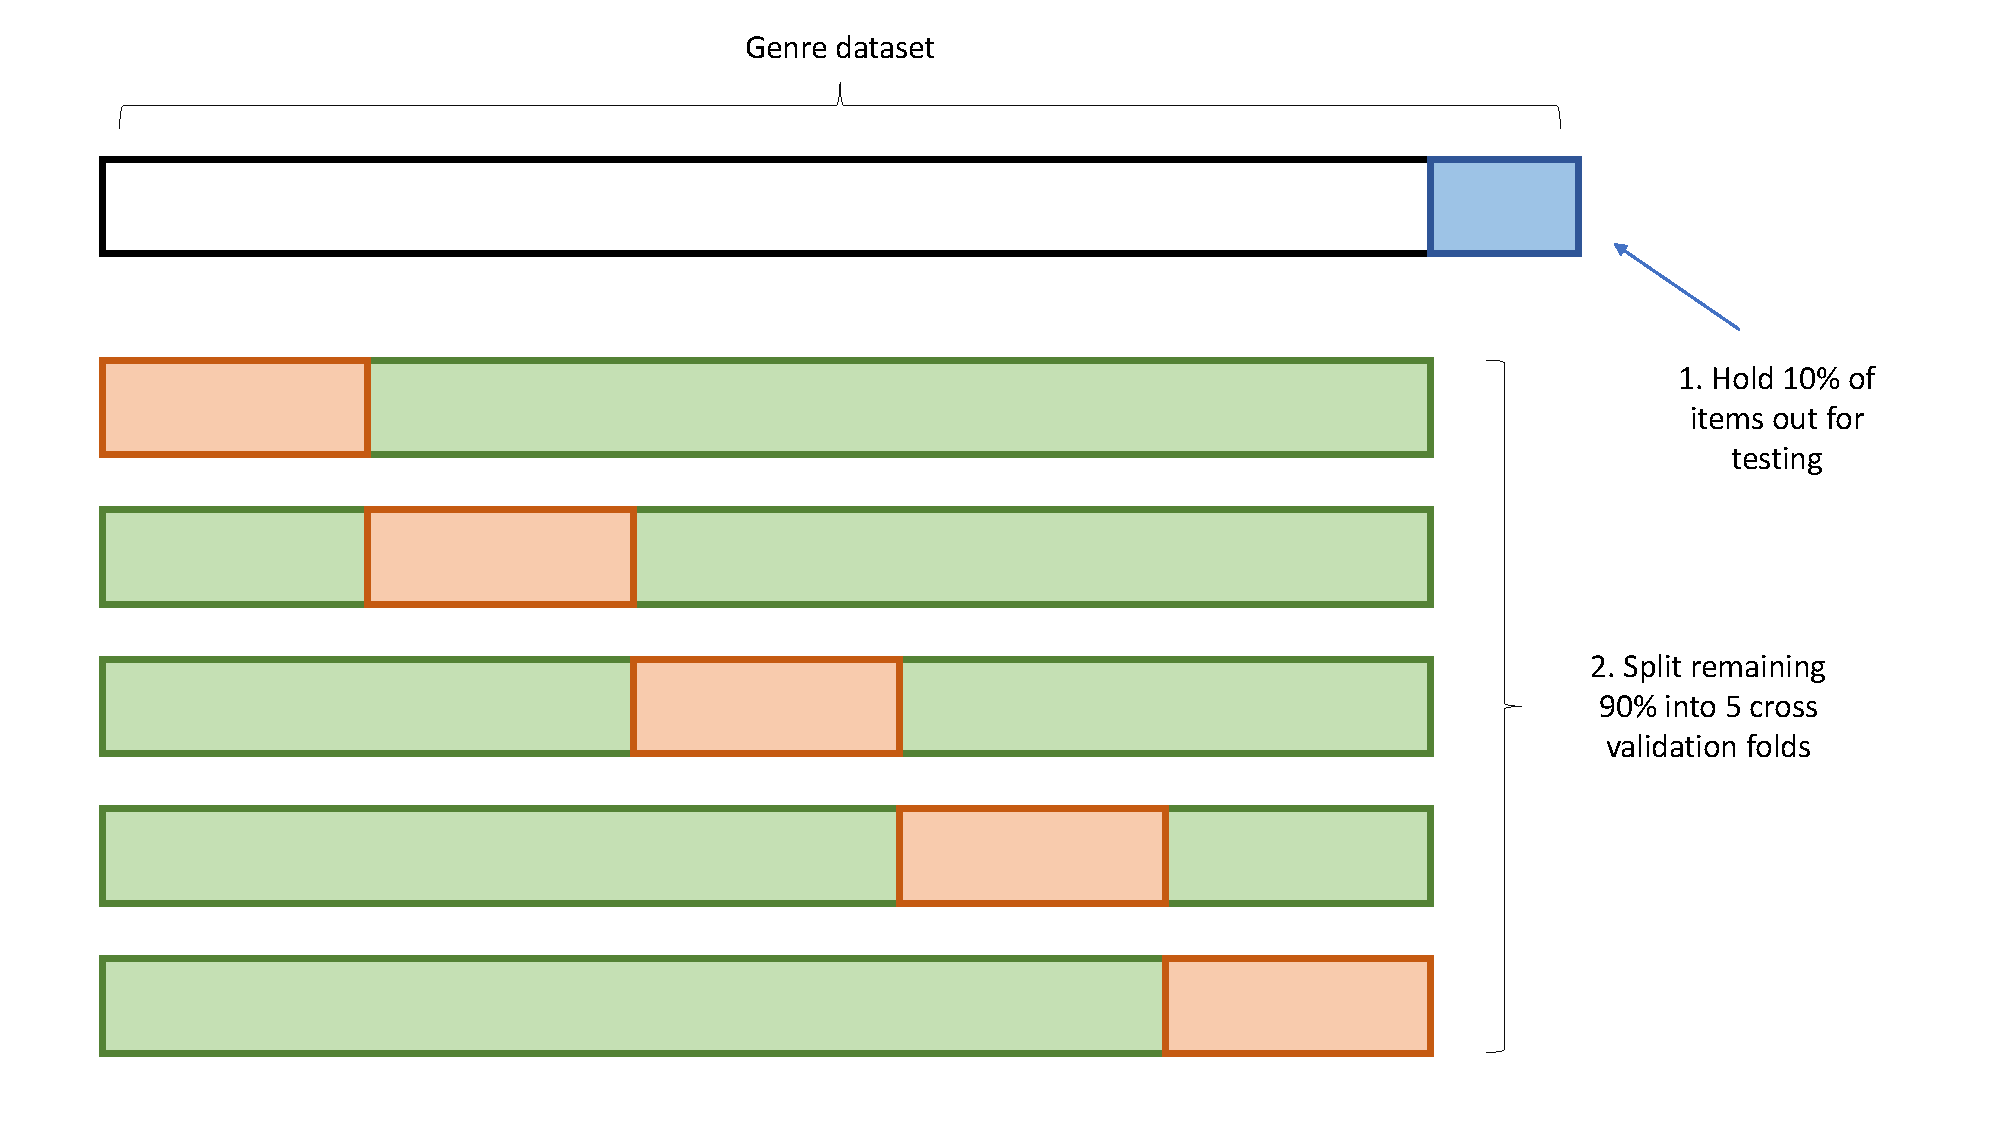
\includegraphics[width=0.85\textwidth]{Figures/4_cross-validation-2.pdf}
\decoRule
\caption[Holdout set]{10\% of the genre labels (blue) were removed from the dataset \textit{before} performing cross validation. In each fold, the model was trained on 80\% (green) and validated on the remaining 20\% (orange).}
\label{fig:4_cross-validation}
\end{figure}

For a given configuration of the model, 5 separate instances of training need to be performed, using a different fold each time. The model is then evaluated by taking the average holdout performance across the 5 folds. Training in this way allows for a more robust measure of performance than a single 80/20 split, while enabling the use of all available data for training.

\subsection{Hyperparameter tuning}
Tuning the hyperparameters of the two models was done using a grid search, in which a wide range of different combinations of hyperparameters was tested. For each combination of hyperparameters, the two models were trained sequentially. The rating model was trained on all available rating data, before the genre model was trained and assessed on 5 CV splits. The performance of each configuration was taken as the average validation fold loss of the genre model. The hyperparameters chosen in the rating model were those that led to the best performance in the subsequent genre model. In this way, the rating model was tuned with the objective of maximising the descriptiveness of the embedding layer, rather than the ability to predict user ratings.

The order of operations for the grid search is outlined below:

\begin{enumerate}
  \item For every given combination of hyperparameters:
  \begin{enumerate}
    \item Train rating model on all rating data
    \item Freeze item embedding layer
    \item Create five sequential 80/20 CV folds (as shown in figure \ref{fig:4_cross-validation})
    \item Train and assess genre model on each CV fold
    \item Record performance as average validation loss across all folds
  \end{enumerate}
  \item Choose best performing combination of hyperparameters
\end{enumerate}

A separate model was trained using every possible combination of hyperparameters and validated on each of the 5 folds. The rating model was trained on all data, before the item embedding layer was frozen and used in the genre model. The model with the best average holdout performance across the 5 folds was chosen as the best performer.

The results of hyperparameter tuning and evaluation are detailed in the next chapter.
\chapter{Results and Analysis}
\label{results}

This chapter details the results of tuning and evaluating the CGT model. All available user-item ratings were used to tune the rating model, while 90\% of the movie genre labels were used to train and tune the genre model. Only the "drama" label was used in the MovieLens datasets, as it was the most evenly balanced class. Goodbooks-10k used only the "adult-fiction" label, which had very close to 50/50 class weighting. The chapter concludes with an exploratory analysis of the item latent factors.

\section{Hyperparameter grid search}
A number of grid searches were performed to tune the hyperparameters of the CGT model. Due to the different sizes of the MovieLens (ML) datasets, the smallest dataset, ML100k, was used to test the widest range of hyperparameters. Then, a subset of the best-performing hyperparameters were tested again on the ML1M dataset. No hyperparameter tuning was done on ML10M due to its size. The best hyperparameters from ML1M were used for ML10M and GB10k.

In each grid search, the best parameters were chosen as those which minimised the average CV log loss of the genre classifications.

When initialising weights of each model, the same random seed was used to allow for reproducible results.

\subsection{MovieLens100k}
Four grid searches were performed on the ML100k dataset. The first grid search tested various combinations of $k$ -- the number of latent factors, $h$ -- the number of hidden nodes in the rating model, and $j$ -- the number of hidden nodes in the genre model. The second grid search tested different numbers of training epochs and the third tested different values of $dr1$ and $dr2$ -- the dropout rate in the hidden layers of each model. Finally, a number of different activation functions were tested. Each successive hyperparameter search used the best set of hyperparameters from the previous.

\subsubsection{Number of latent factors and hidden neurons}
Values between 50 and 200 were tested for $k$, while $h$ and $j$ were tested in the range of 25 and 100. While tuning these parameters, the dropout rate of the hidden layers, $dr1$ and $dr2$ were both fixed at 0.2 and ReLU was used as the activation function. A total of 12 different combinations were tested in this grid search, the top 5 models are shown in table \ref{tab:ml100k-grid-results1}.

\begin{table}[H]
\centering
\begin{tabular}{c | c | c | c | c}
\toprule
\textbf{$k$} & \textbf{$h$} & \textbf{$j$} & \textbf{Avg. CV log loss} & \textbf{Avg. CV acc.} \% \\
\midrule
200 & 100 & 100 & 0.6344 & 63.12 \\
\midrule
200 & 100 & 50 & 0.6365 & 62.52 \\
\midrule
100 & 100 & 100 & 0.6391 & 62.79 \\
\midrule
100 & 50 & 100 & 0.6394 & 62.39 \\
\midrule
200 & 50 & 100 & 0.6406 & 62.85 \\
\bottomrule
\end{tabular}
\caption[MovieLens 100k grid search results -- number of nodes]{Results of first grid search performed on ML100k. Average CV log loss and accuracy are shown for different combinations of $k$, $h$ and $j$.}
\label{tab:ml100k-grid-results1}
\end{table}

The best performing set of hyperparameters in the first grid search was $k=200$, $h=100$ and $j=100$. All of the top five used a latent factor vector size of either 100 or 200. All top three models had a value of 100 for $h$, while four of the top five had a value of 100 for $j$. The relationship between the size of $k$ and the average CV loss is shown in figure \ref{fig:5-latent-size}

\begin{figure}[H]
\centering
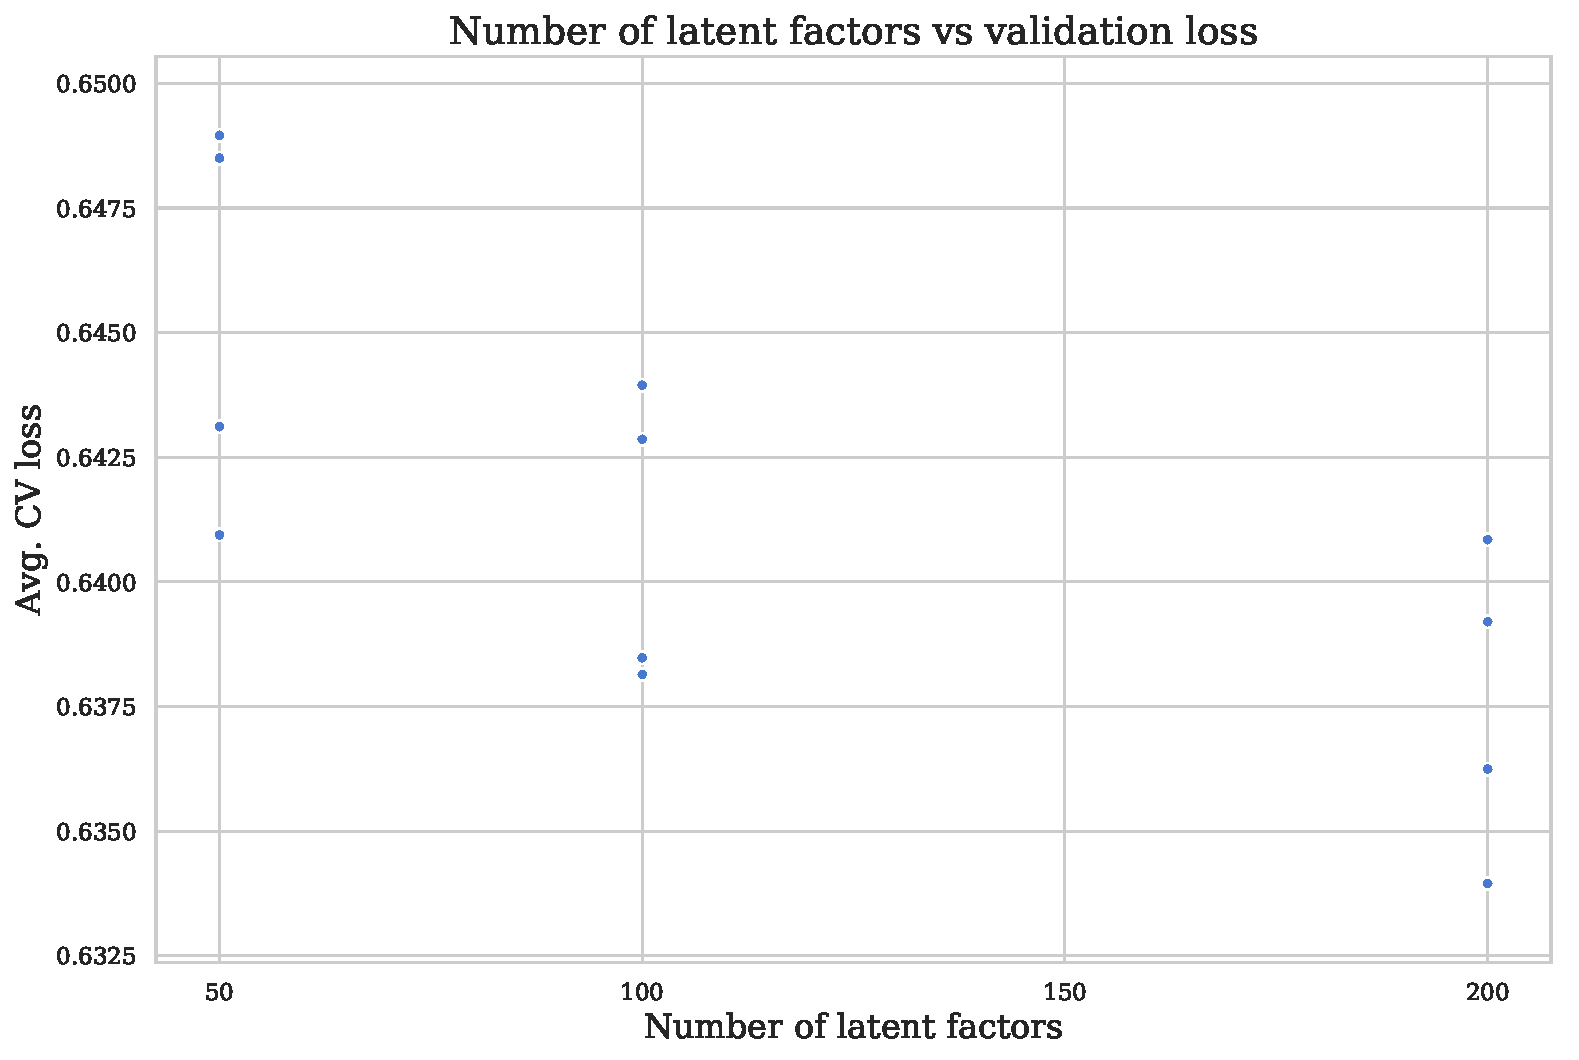
\includegraphics[width=0.78\textwidth]{Figures/5_ml100k-latent-factors.pdf}
\decoRule
\caption[Number of latent factors vs classification accuracy]{Relationship between number of latent factors and classification performance.}
\label{fig:5-latent-size}
\end{figure}

\subsubsection{Number of epochs}
Training the model for too many epochs could risk overfitting. Therefore, it was necessary to find the optimal number of epochs for both the rating and genre model. Values of 5, 6 and 7 were tested for the rating model, while values of 3, 4 and 5 were tested for the genre model. This meant a total of 9 different combinations were tested in this grid search, with each one using the hyperparameters $k$, $h$ and $j$ from the best performing model in the first grid search. The top 5 models are shown in table \ref{tab:ml100k-grid-results2}. $E1$ and $E2$ are the number of epochs used for the rating and genre model respectively.

\begin{table}[H]
\centering
\begin{tabular}{c | c | c | c}
\toprule
\textbf{$E1$} & \textbf{$E2$} & \textbf{Avg. CV log loss} & \textbf{Avg. CV acc.} \% \\
\midrule
7 & 5 & 0.6344 & 63.12 \\
\midrule
6 & 5 & 0.6353 & 63.19 \\
\midrule
7 & 4 & 0.6360 & 63.12 \\
\midrule
6 & 4 & 0.6366 & 63.32 \\
\midrule
5 & 5 & 0.6376 & 62.72 \\
\bottomrule
\end{tabular}
\caption[MovieLens 100k grid search results -- number of epochs]{Results of third ML100k grid search which tested  different combinations of $E1$ and $E2$.}
\label{tab:ml100k-grid-results2}
\end{table}

\subsubsection{Dropout rates}
The third grid search tested different combinations of dropout rates used in the hidden layers of the two models. Values between 0.15 and 0.25 were tested. A total of 9 different combinations were tested in this grid search. The top 5 models from the third grid search are shown in table \ref{tab:ml100k-grid-results3}.

\begin{table}[H]
\centering
\begin{tabular}{c | c | c | c | c}
\toprule
\textbf{$dr1$} & \textbf{$dr2$} & \textbf{Avg. CV log loss} & \textbf{Avg. CV acc.} \% \\
\midrule
0.25 & 0.15 & 0.6334 & 62.99 \\
\midrule
0.25 & 0.2 & 0.6336 & 63.32 \\
\midrule
0.25 & 0.25 & 0.6337 & 63.19 \\
\midrule
0.2 & 0.15 & 0.6343 & 63.05 \\
\midrule
0.2 & 0.2 & 0.6344 & 63.12 \\
\bottomrule
\end{tabular}
\caption[MovieLens 100k grid search results -- dropout rates]{Results of third ML100k grid search which tested different combinations of $dr1$ and $dr2$.}
\label{tab:ml100k-grid-results3}
\end{table}

The best performing model used a higher dropout rate of 0.25 in the rating model, compared to 0.15 in the genre model.

\subsubsection{Activation function}
Finally, five different activation functions were tested using the best parameters from the first three grid searches. The five activation functions used were:
\begin{itemize}
    \item Linear
    \item Rectified Linear Unit (ReLU)
    \item Scaled Exponential Linear Unit (SELU)
    \item Softplus
    \item Hyperbolic tangent (Tanh)
\end{itemize}
The CV performance of each activation function is shown in \ref{tab:ml100k-activations}.

\begin{table}[H]
\centering
\begin{tabular}{c | c | c | c | c}
\toprule
\textbf{Activation function} & \textbf{Avg. CV log loss} & \textbf{Avg. CV acc.} \% \\
\midrule
ReLU & 0.6334 & 63.12 \\
\midrule
Softplus & 0.6461 & 60.81 \\
\midrule
SELU & 0.6467 & 60.67 \\
\midrule
Tanh & 0.6494 & 59.95 \\
\midrule
Linear & 0.6500 & 59.42 \\
\bottomrule
\end{tabular}
\caption[MovieLens 100k grid search results -- activation function]{Comparison of activation functions}
\label{tab:ml100k-activations}
\end{table}

\subsection{MovieLens1M}
A second set of grid searches was performed on MovieLens1M, using a subset of the best performing values tested on MovieLens100k. The parameters tested on ML1M included the number of latent factors, number of hidden neurons, number of training epochs, and the dropout rates. The ReLU activation function was chosen for this dataset, as it was significantly better than the other four that were tested on ML100k.

\subsubsection{Number of latent factors and hidden neurons}
Values of 100 and 200 were tested for $k$, while $h$ and $j$ were tested between 50 and 100. This totalled 8 different combinations, of which the top 5 models are shown in table \ref{tab:ml1m-grid-results1}.

\begin{table}[H]
\centering
\begin{tabular}{c | c | c | c | c}
\toprule
\textbf{$k$} & \textbf{$h$} & \textbf{$j$} & \textbf{Avg. CV log loss} & \textbf{Avg. CV acc.} \% \\
\midrule
200 & 100 & 100 & 0.5815 & 69.00 \\
\midrule
200 & 100 & 50 & 0.5947 & 67.92 \\
\midrule
200 & 50 & 100 & 0.5997 & 66.78 \\
\midrule
100 & 100 & 100 & 0.6013 & 66.33 \\
\midrule
200 & 50 & 50 & 0.6058 & 66.00 \\
\bottomrule
\end{tabular}
\caption[MovieLens 1M grid search results -- number of nodes]{Best values of $k$, $h$ and $j$ on MovieLens 1M dataset.}
\label{tab:ml1m-grid-results1}
\end{table}

As was the case with ML100k, the best values for $k$, $h$ and $j$ for ML1M were 200, 100 and 100 respectively.

\subsubsection{Number of epochs}
Values of 7 and 8 were tested for $E1$ and 5, 6 and 7 were tested for $E2$. The top 5 combinations of $E1$ and $E2$ are shown in table \ref{tab:ml1m-grid-results2}.

\begin{table}[H]
\centering
\begin{tabular}{c | c | c | c}
\toprule
\textbf{$E1$} & \textbf{$E2$} & \textbf{Avg. CV log loss} & \textbf{Avg. CV acc.} \% \\
\midrule
8 & 7 & 0.5714 & 69.12 \\
\midrule
8 & 6 & 0.5728 & 69.50 \\
\midrule
8 & 5 & 0.5761 & 69.92 \\
\midrule
7 & 7 & 0.5767 & 68.86 \\
\midrule
7 & 6 & 0.5783 & 68.94 \\
\bottomrule
\end{tabular}
\caption[MovieLens 1M grid search results -- number of epochs]{Number of training epochs for both models on ML1M.}
\label{tab:ml1m-grid-results2}
\end{table}

\subsubsection{Dropout rates}
The same values of $d1$ and $d2$ that were tested on ML 100k were tested again on this dataset, the results are shown below in table \ref{tab:ml1m-grid-results3}.

\begin{table}[H]
\centering
\begin{tabular}{c | c | c | c | c}
\toprule
\textbf{$dr1$} & \textbf{$dr2$} & \textbf{Avg. CV log loss} & \textbf{Avg. CV acc.} \% \\
\midrule
0.15 & 0.15 & 0.5664 & 69.69 \\
\midrule
0.15 & 0.2 & 0.5665 & 69.63 \\
\midrule
0.15 & 0.25 & 0.5668 & 69.81 \\
\midrule
0.25 & 0.15 & 0.5693 & 70.49 \\
\midrule
0.25 & 0.2 & 0.5695 & 70.37 \\
\bottomrule
\end{tabular}
\caption[MovieLens 1M grid search results -- dropout rates]{Best 5 dropout rates on MovieLens 1M dataset.}
\label{tab:ml1m-grid-results3}
\end{table}

Unlike the ML100k grid search, lower dropout rates yielded the lowest CV loss on ML1M. A value of 0.15 used as the dropout rate in both the rating and genre model resulted in the best performing model.

\section{Holdout testing}
After tuning hyperparemeters, CGT was tested against the 10\% holdout set for each of the three MovieLens datasets and the Goodbooks-10k dataset. For ML10M and Goodbooks-10k, the model was trained on 90\% of the data, using the best hyperparameters from the ML1M model, i.e. without tuning any hyperparameters.

\subsection{Classification metrics}
Performance on the holdout set was evaluated using four different classification metrics, namely accuracy, precision, recall and F1 score. The test results are shown in table \ref{tab:ml-test-results} below for all four datasets. Class weight refers to the number of movies in the holdout set which had a positive class label. For example, the holdout set in ML100k consisted of a total of 169 movies, of which 73 were dramas. 495 of the 1000 books in the Goodbooks-10k dataset had the "adult-fiction" label.

\begin{table}[H]
\centering
\begin{tabular}{c | c | c | c | c | c | c}
\toprule
\textbf{Dataset} & \textbf{Class weight} & \textbf{Accuracy} & \textbf{Precision} & \textbf{Recall} & \textbf{F1 score} \\
\midrule
ML 100k & 73/169 (43\%) & 0.63 & 0.58 & 0.52 & 0.55 \\
\midrule
ML 1M & 144/371 (39\%) & 0.70 & 0.61 & 0.61 & 0.61 \\
\midrule
ML 10M & 517/1068 (48\%) & 0.70 & 0.68 & 0.70 & 0.69 \\
\midrule
GB 10k & 495/1000 (50\%) & 0.63 & 0.63 & 0.59 & 0.61 \\
\bottomrule
\end{tabular}
\caption[Holdout classification report]{Classification performance of CGT.}
\label{tab:ml-test-results}
\end{table}

One can see above that the classification accuracy increases with the size of the dataset. ML 100k has the worst performance with 63\% of the movies correctly labelled. ML 10M, which also has the most even split between positive and negative labels (drama vs not drama), has the best performance with 70\% accuracy and an F1 score of 0.69.

\subsection{Confusion matrices}
To further break down the performance of the genre prediction, confusion matrices show the relationship between predicted and actual labels for the movies. The confusion matrices for each data set are given in tables \ref{tab:ml100k-confusion-matrix}, \ref{tab:ml1m-confusion-matrix}, \ref{tab:ml10m-confusion-matrix} and \ref{tab:gb10k-confusion-matrix} below. In each matrix, the columns represent the predicted labels and the rows represent the actual labels.

\begin{table}[H]
\centering
\begin{tabular}{c | c | c | c}
\toprule
 & \textbf{Negative} & \textbf{Positive} & \textbf{Total} \\
\midrule
\textbf{Negative} & 68 & 28 & 96 \\
\midrule
\textbf{Positive} & 35 & 38 & 73 \\
\midrule
\textbf{Total} & 103 & 66 & 169 \\
\bottomrule
\end{tabular}
\caption[MovieLens 100k confusion matrix]{Confusion matrix of ML100k holdout set.}
\label{tab:ml100k-confusion-matrix}
\end{table}

\begin{table}[H]
\centering
\begin{tabular}{c | c | c | c}
\toprule
 & \textbf{Negative} & \textbf{Positive} & \textbf{Total} \\
\midrule
\textbf{Negative} & 170 & 57 & 227 \\
\midrule
\textbf{Positive} & 56 & 88 & 144 \\
\midrule
\textbf{Total} & 226 & 145 & 371 \\
\bottomrule
\end{tabular}
\caption[MovieLens 1M confusion matrix]{Confusion matrix of ML1M holdout set.}
\label{tab:ml1m-confusion-matrix}
\end{table}

\begin{table}[H]
\centering
\begin{tabular}{c | c | c | c}
\toprule
 & \textbf{Negative} & \textbf{Positive} & \textbf{Total} \\
\midrule
\textbf{Negative} & 384 & 167 & 551 \\
\midrule
\textbf{Positive} & 154 & 363 & 517 \\
\midrule
\textbf{Total} & 538 & 530 & 1068 \\
\bottomrule
\end{tabular}
\caption[MovieLens 10M confusion matrix]{Confusion matrix of ML10M holdout set.}
\label{tab:ml10m-confusion-matrix}
\end{table}

\begin{table}[H]
\centering
\begin{tabular}{c | c | c | c}
\toprule
 & \textbf{Negative} & \textbf{Positive} & \textbf{Total} \\
\midrule
\textbf{Negative} & 337 & 168 & 505 \\
\midrule
\textbf{Positive} & 205 & 290 & 495 \\
\midrule
\textbf{Total} & 542 & 458 & 1000 \\
\bottomrule
\end{tabular}
\caption[Goodbooks-10k confusion matrix]{Confusion matrix of GB10k holdout set.}
\label{tab:gb10k-confusion-matrix}
\end{table}

\subsection{Number of ratings per item}
Looking at table \ref{tab:ratings-distribution}, one can see that ML10M has the highest average number of ratings per item, 937, compared to only 60 ratings per item in ML100k. Intuitively, the better performance on the dataset with more ratings per movie makes sense as each user-item interaction provides an additional training observation for training item latent factors.

The relationship between number of user ratings and classification accuracy was investigated by binning movies by rating count and then taking the average accuracy for each bin. The results of this investigation are shown in figure \ref{fig:5-ratings-vs-acc}. Each bar represents a single bin's mean classification accuracy. Blue bars are for training data and orange represents testing data. The ranges for the bins were chosen to ensure a minimum of 20 test observations in each bin.

\begin{figure}[H]
\centering
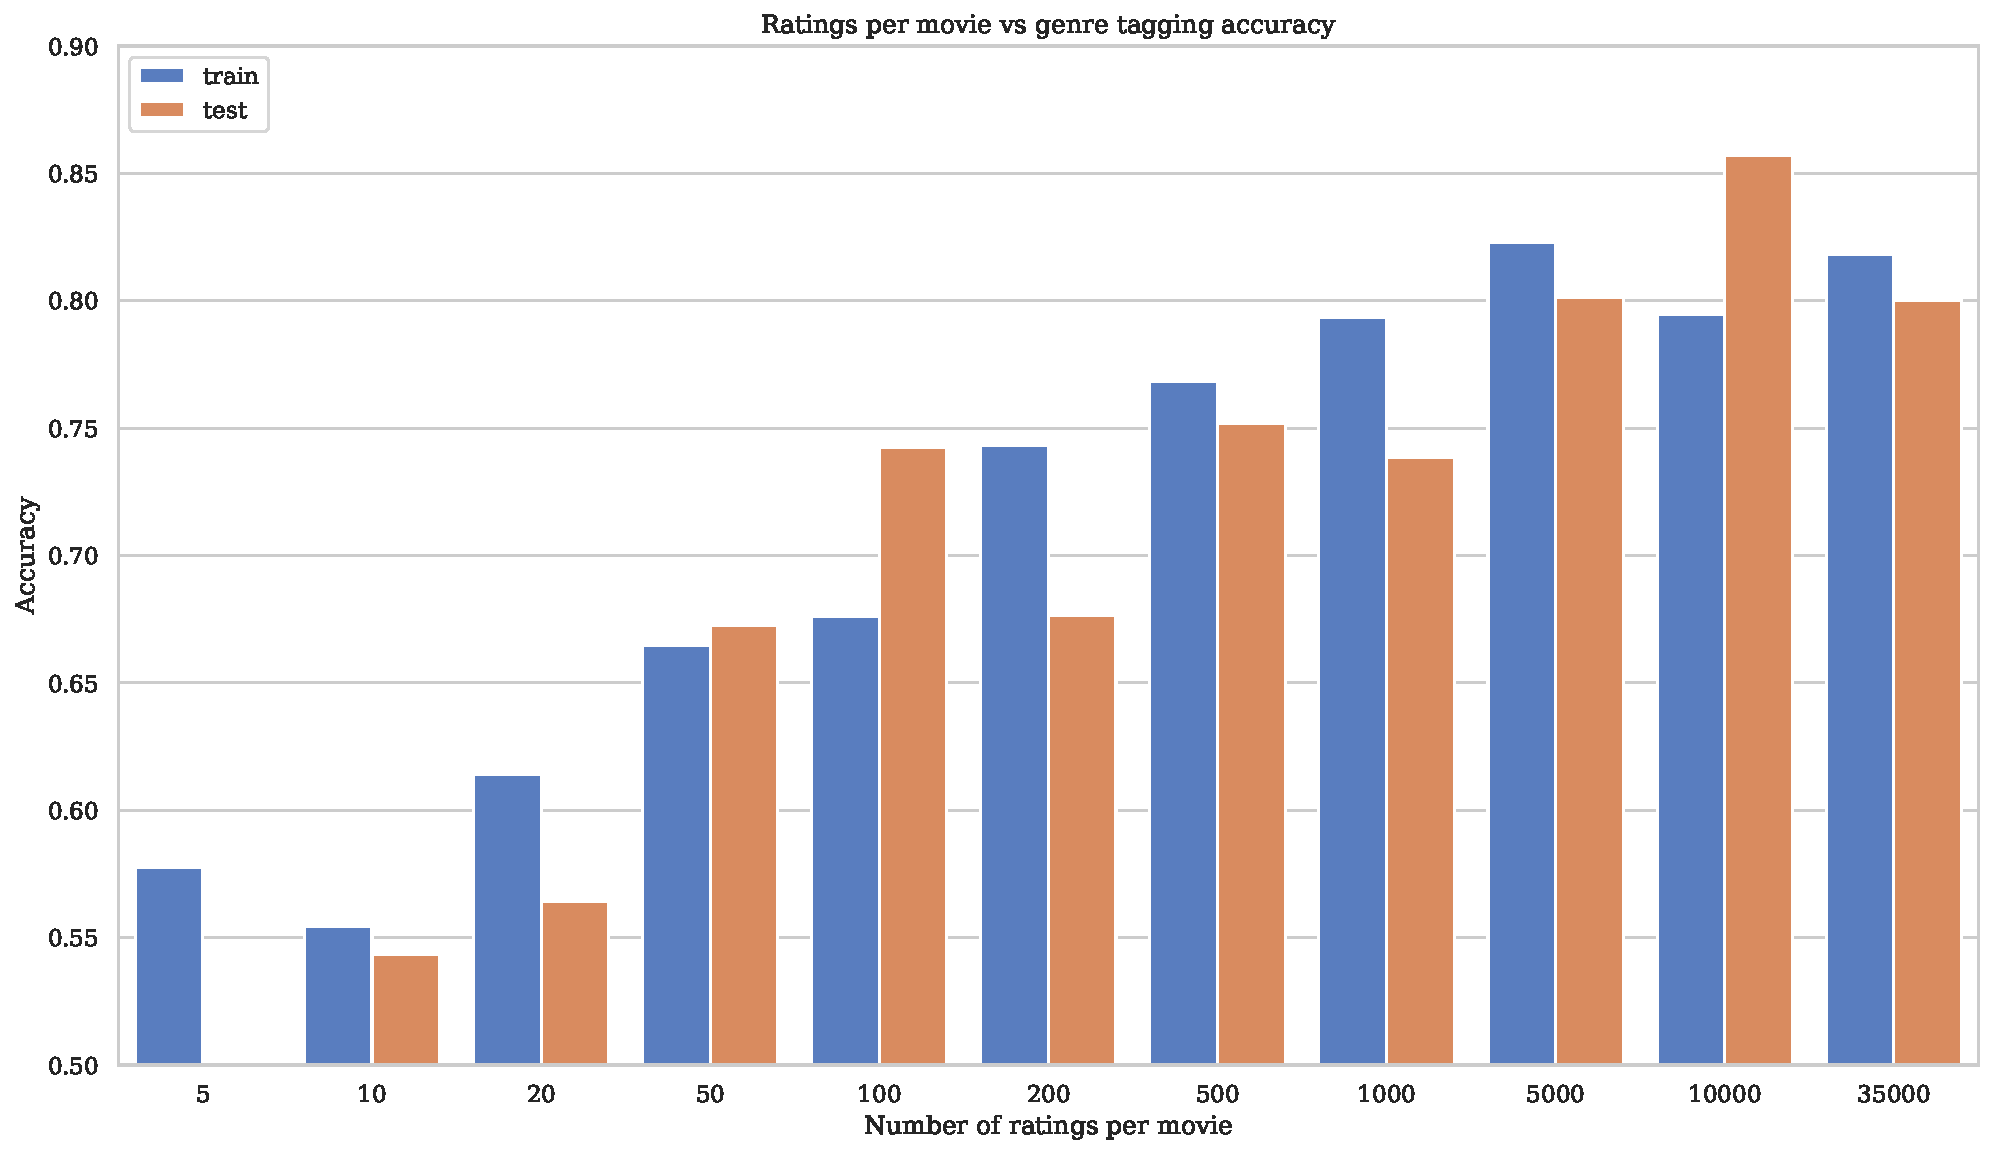
\includegraphics[width=0.85\textwidth]{Figures/5_ml10m-ratings-vs-acc.pdf}
\decoRule
\caption[Number of ratings vs accuracy]{Movies with more ratings tend to be more accurately classified.}
\label{fig:5-ratings-vs-acc}
\end{figure}

It can be seen in figure \ref{fig:5-ratings-vs-acc} that as the number of ratings per movie increases, the accuracy with which CGT can predict its genre increases too. For movies with 5000 or more ratings, the average classification accuracy is over 80\%.

\section{Latent factor analysis}
To understand the relationship between the latent factors in the embedding layer and genres in ML10M, the item embedding matrix was reduced from 200 dimensions to 2. Dimensionality reduction was done using principal component analysis, in which the 200-dimensional space of the embedding matrix was decomposed into 2 mutually orthogonal dimensions -- or components -- that captured the maximum amount of variance from the original space. While this reduction in dimensionality inevitably leads to a loss of information, it allows the movies to be visualised in the latent factor space.

\subsection{Distribution of genres}
Figure \ref{fig:5-genre-pca} shows the distribution of two genres, "Children" and "Documentary", in the first two principal components of the latent factor space. Out of the total 10 000 movies in ML10M, 528 are classified in the "Children" genre and 479 are documentaries. There are only 2 movies which are labelled as both a children's film and a documentary.

\begin{figure}[H]
\centering
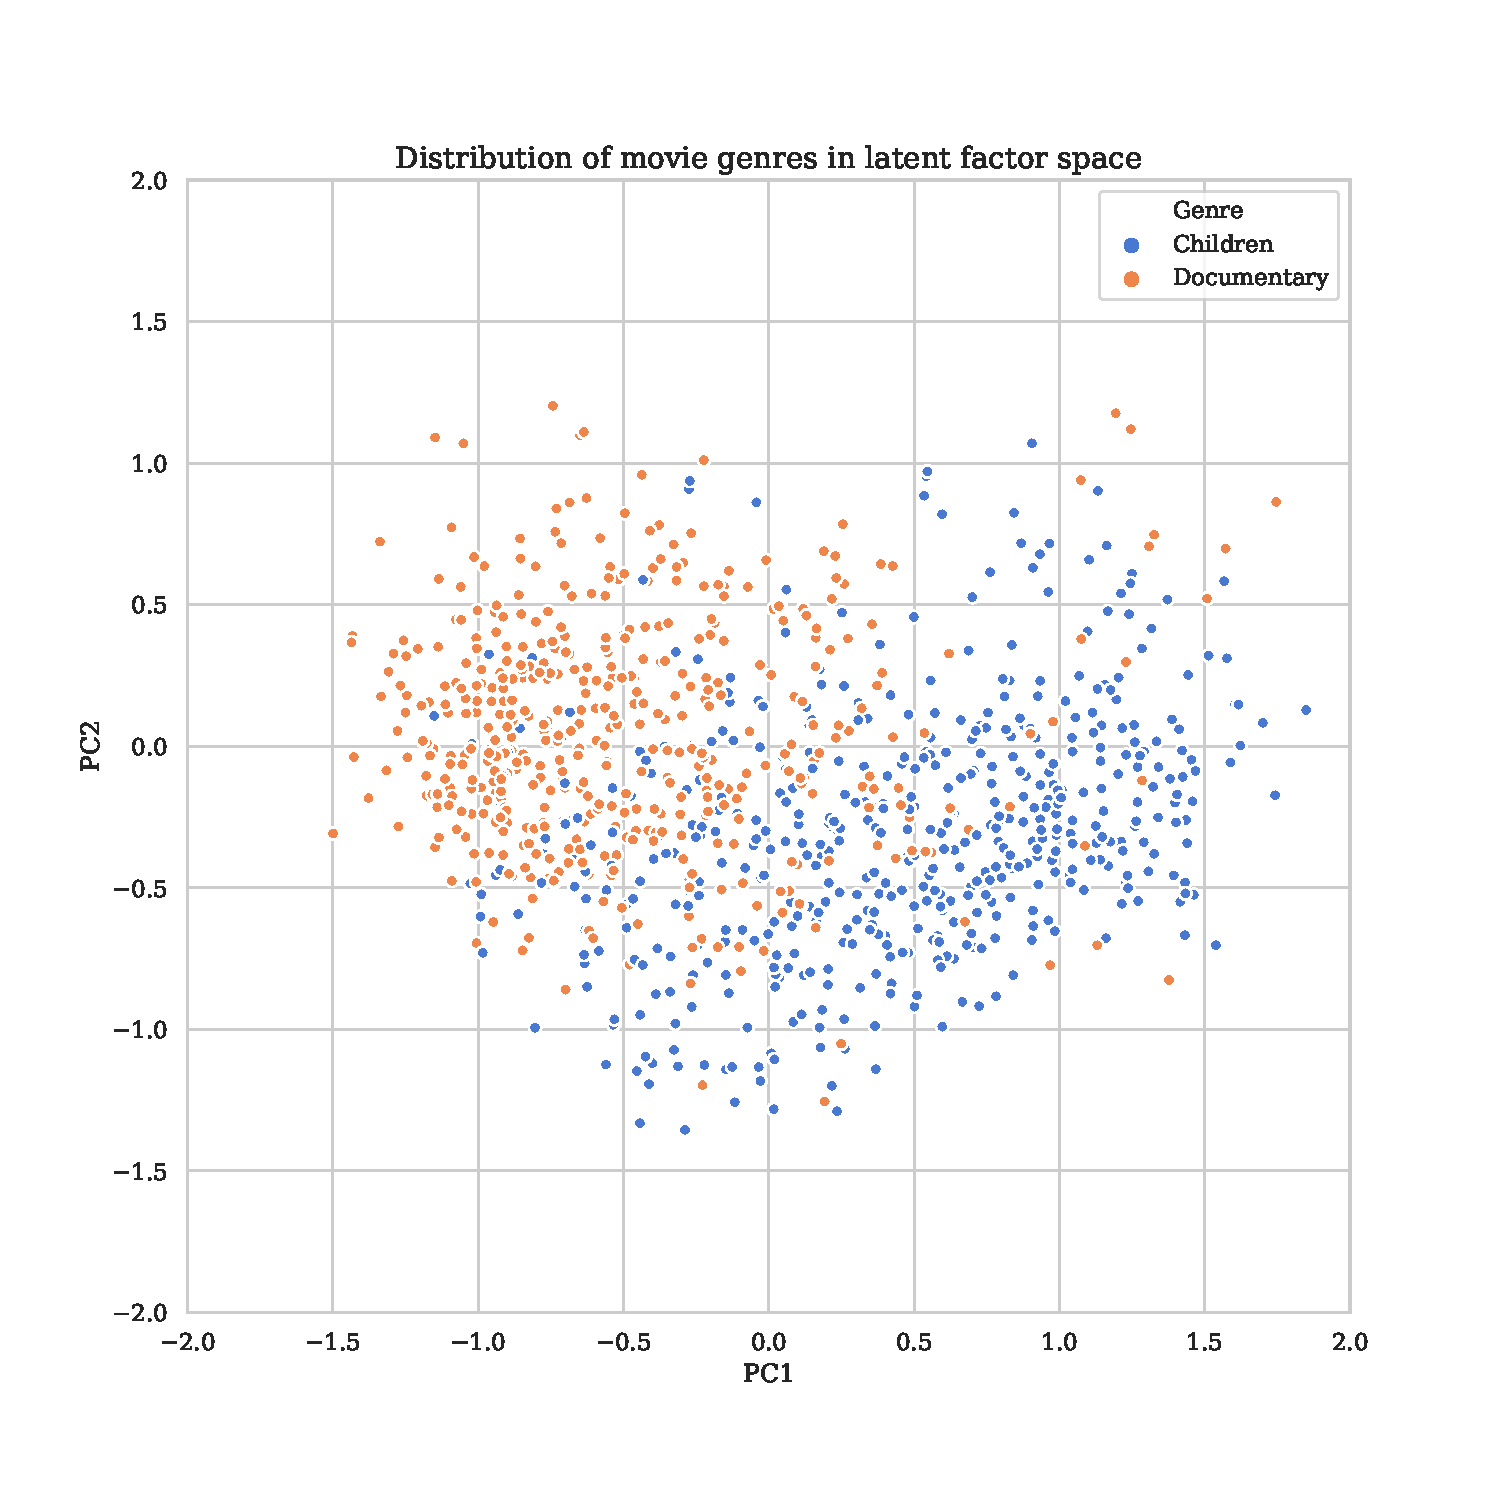
\includegraphics[width=0.7\textwidth]{Figures/5_ml10m-genre-pca.pdf}
\decoRule
\caption[Distribution of genres in latent factor space]{Children's movies and documentaries shown in the first two principal components of the latent factor space.}
\label{fig:5-genre-pca}
\end{figure}

Although the genre model was not trained to predict either of these genres, this figure serves to illustrate the inherent ability of the latent factors to capture descriptive features of movies. While not entirely separable, the difference in principal component loadings between these two genres can be seen in just two dimensions. The geometric means of each genre are given in table \ref{tab:ml10m-genre-pca}

\begin{table}[H]
\centering
\begin{tabular}{c | c | c}
\toprule
\textbf{Genre} & \textbf{$\Bar{PC1}$} & \textbf{$\Bar{PC2}$} \\
\midrule
Children & 0.437 & -0.300 \\
\midrule
Documentary & -0.477 & 0.046 \\
\bottomrule
\end{tabular}
\caption[Genre principal component means]{Geometric means of "Children" and "Documentary" genres in first two principal components of latent factor space.}
\label{tab:ml10m-genre-pca}
\end{table}

It is shown above that the centre of "Children" genre has a moderately strong positive loading in the first principal component, while the centre of the "Documentary" genre has a similarly strong negative loading.

\subsection{Distribution of ratings}
Figure \ref{fig:5-ratings-scatter} shows the 10 highest rated movies alongside the 10 lowest rated movies. There is a clear separation between these two groups.

\begin{figure}[H]
\centering
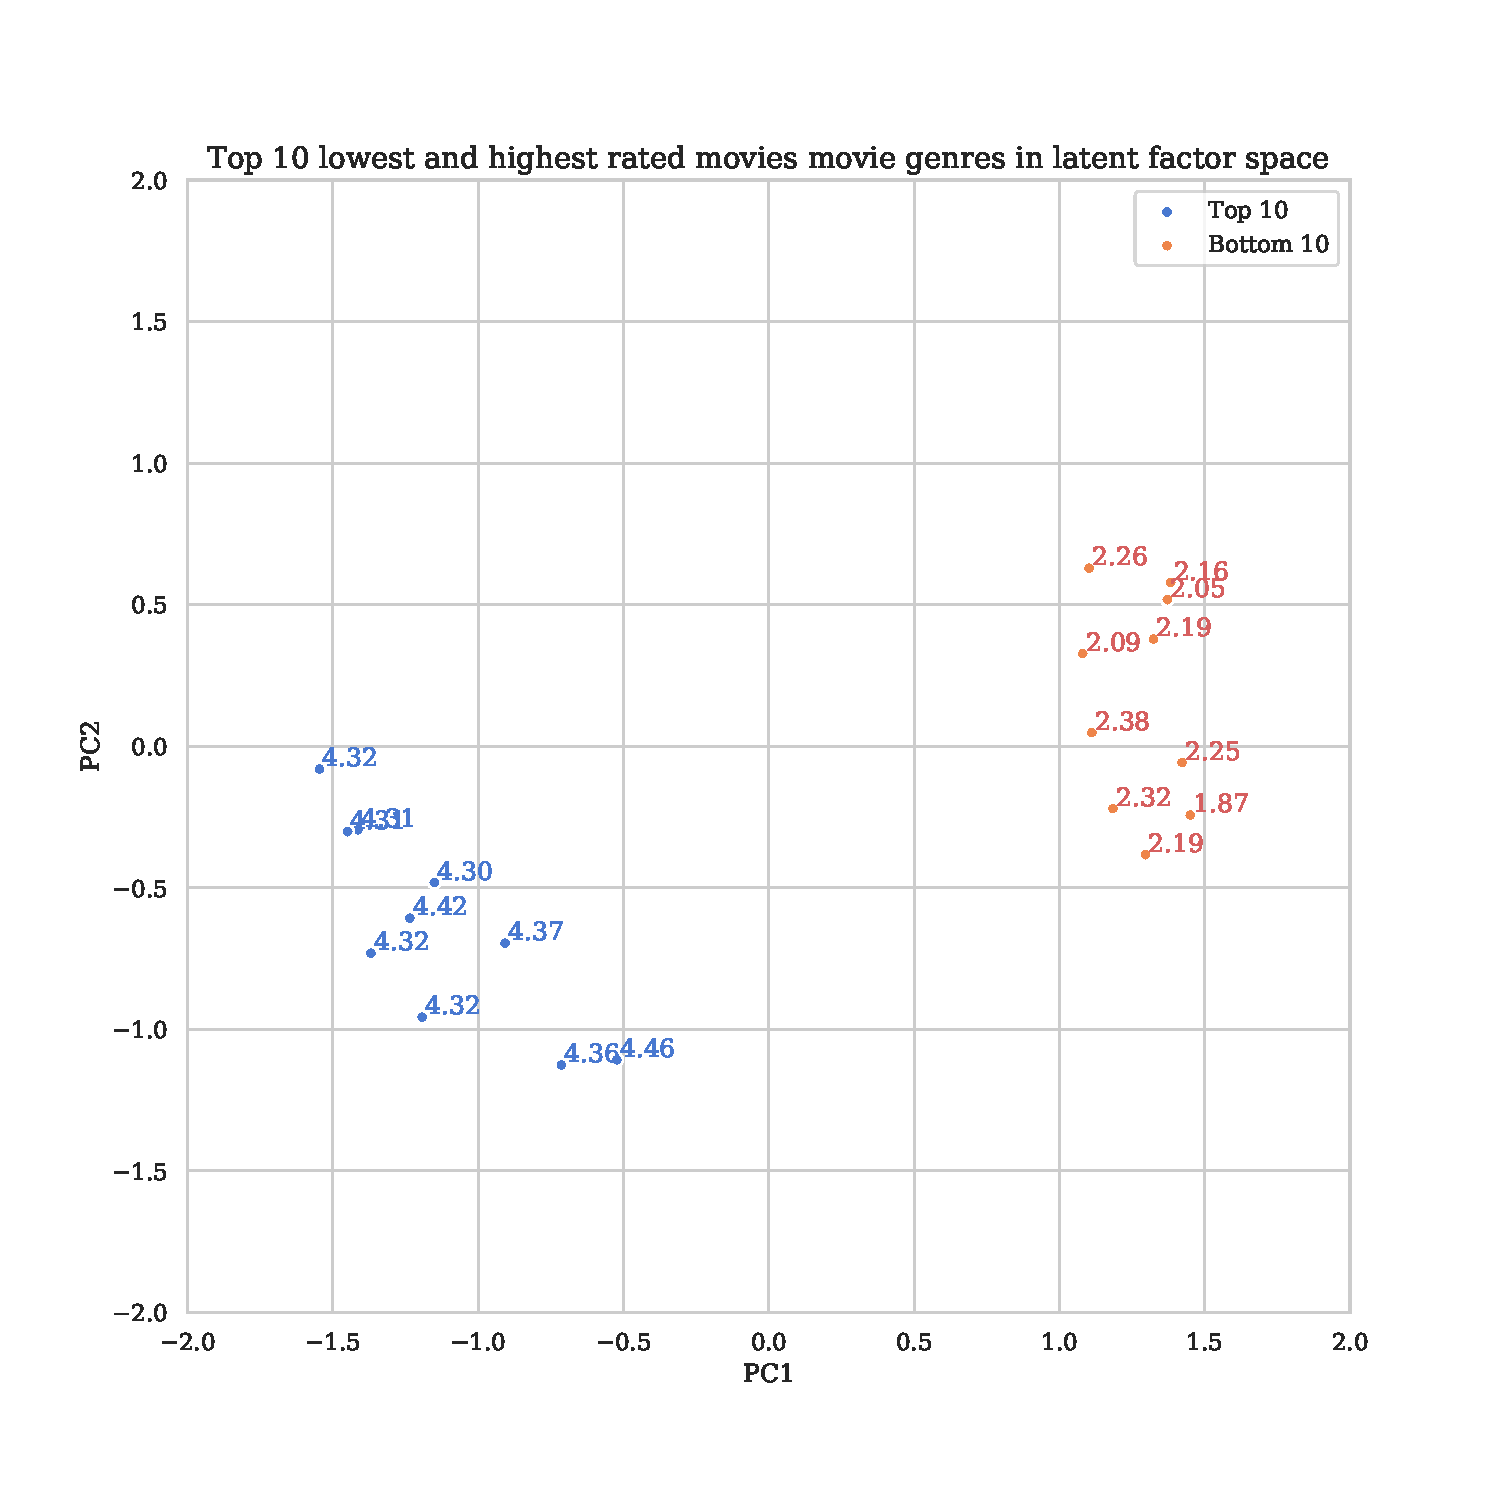
\includegraphics[width=0.69\textwidth]{Figures/5_ml10m-ratings-scatter.pdf}
\decoRule
\caption[Top 10 highest and lowest rated movies]{Top 10 highest (blue) and lowest (red) rated movies in first two principal components. Each point is annotated with its average user rating.}
\label{fig:5-ratings-scatter}
\end{figure}

The highest rated movies all have strong negative loadings in the first principal component, while the lowest rated movies all have equally strong positive loadings. Figure \ref{fig:5-ratings-hexbin} provides a visualisation of the average rating of all 10 000 movies in the latent factor space.

The 'hex bin' plot groups movies into hexagons, the boundaries of which are defined in PC1 and PC2. The value of each hexagon is calculated as the mean rating of all movies that fall inside its boundaries. There is a clear pattern of higher rated movies towards the bottom left of the coordinate grid, with the lowest rated movies in the top right.

\begin{figure}[H]
\centering
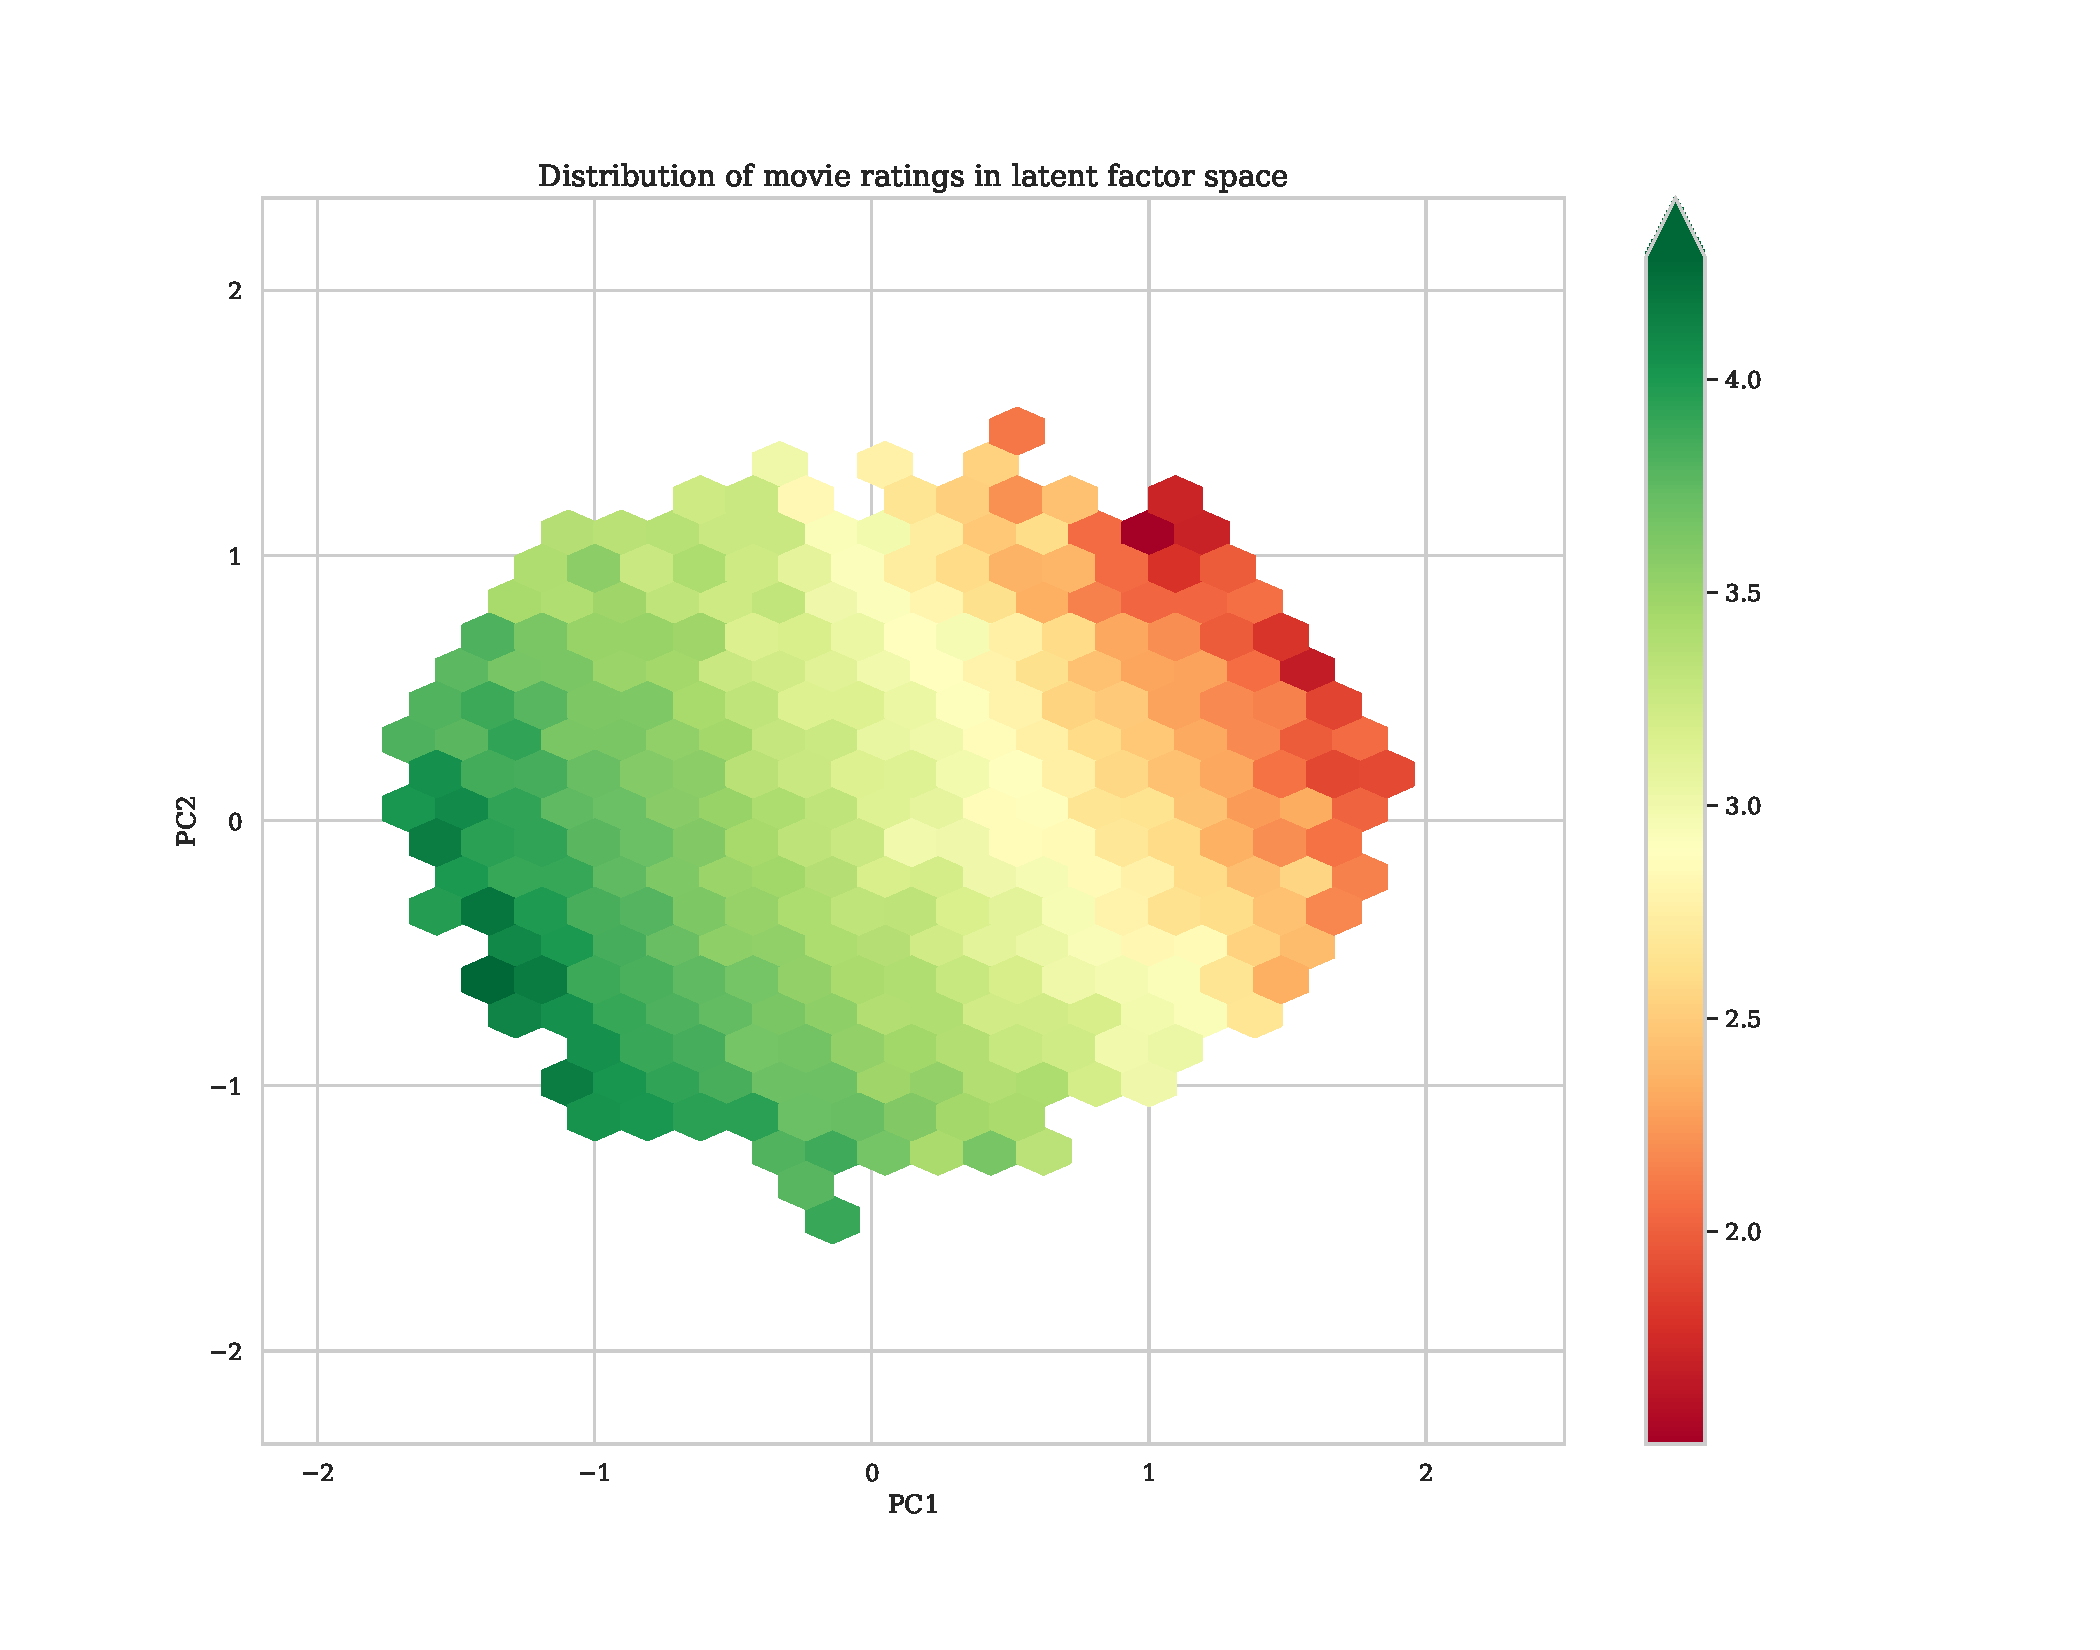
\includegraphics[width=0.74\textwidth]{Figures/5_ml10m-ratings-hexbin.pdf}
\decoRule
\caption[Average rating hex bin plot in PC1 and 2]{Hex bin plot shows average rating within each hexagon. Movies in the bottom left receive higher ratings on average than those in the top right.}
\label{fig:5-ratings-hexbin}
\end{figure}

\subsection{Classification accuracy}
Finally, the relationship between latent factors and classification accuracy was explored. A similar hex bin plot to figure \ref{fig:5-ratings-hexbin} was used, but instead showed the mean classification accuracy in each hexagon. This is shown in figure \ref{fig:5-accuracy-hexbin}.

Interesting to note is the higher accuracies observed at the more extreme loadings of PC1 and PC2. This suggests that movies with more extreme latent factor values are more descriptive and therefore possibly easier to predict. If this is indeed the case, then the goal of the rating model in CGT should be to train latent factors that are maximally dissimilar to each other.

\begin{figure}[H]
\centering
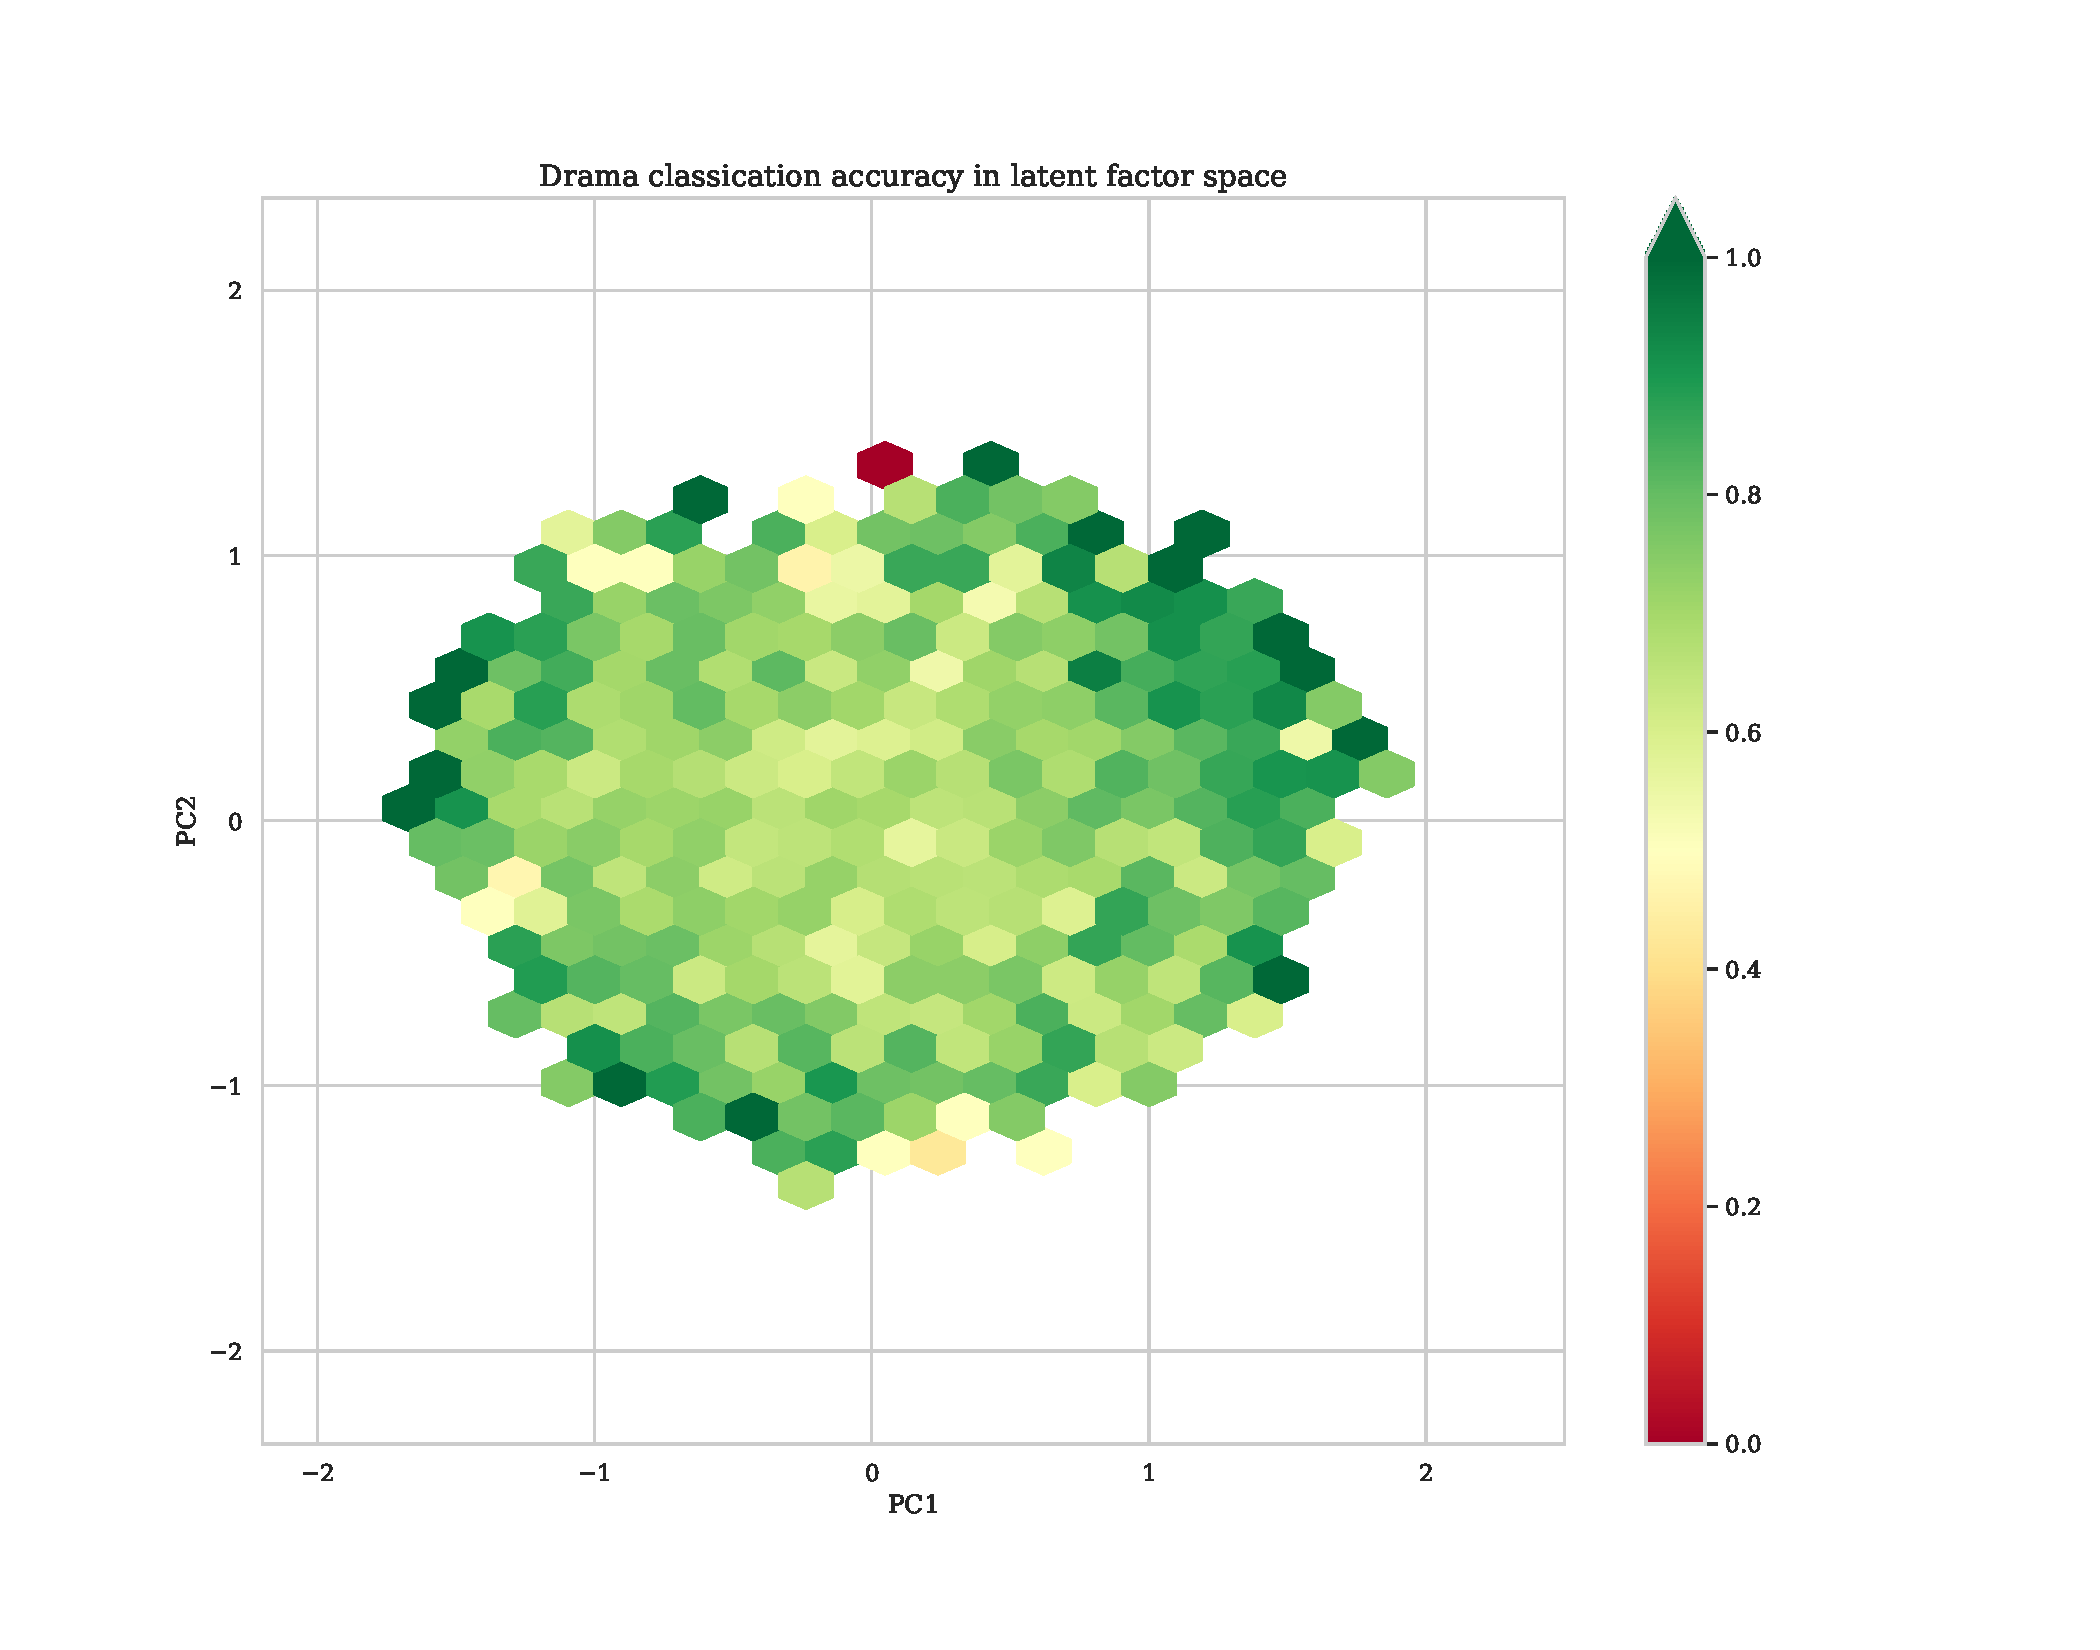
\includegraphics[width=0.74\textwidth]{Figures/5_ml10m-accuracy-hexbin.pdf}
\decoRule
\caption[Classification accuracy hex bin plot in PC1 and 2]{Classification accuracy across PC1 and PC2 of latent factor space. Movies with more extreme latent factors tend to have more extreme accuracy scores.}
\label{fig:5-accuracy-hexbin}
\end{figure}
% \chapter{Conclusions and Recommendations}
\label{conclusions}

\section{Image Classification}

\subsection{Classification Accuracy}
Of the 100 test images, none were incorrectly classified. However, 6 of the 100 images were labelled correctly, but with scores below $70\%$. Of these 6 images, 4 held the true label of 'bin'. In general, the images of bins had a lower average score and the model is more prone to false negatives than false positives. This means that there is a higher chance of an image of a bin being wrongly labelled as background than a background image being labelled as a bin.

\subsection{Error Sources in Classification}
The model was trained using 203 images of bins and 239 background images. The key to training a classifier well is to include varied training imagery which is similar to the images on which the model will eventually be tested. In this project, the training data was collected from GSV images found on Main Road (m4) between the areas of Diep River and Rondebosch in the Cape Town Southern Suburbs area. The testing data was all obtained from images in the central business district area of the city.

It is possible that there are certain patterns in the Street View imagery that differ between images in these two areas. For example, many of the bins in the training set were found on grassy street corners whereas all of the bins in the CBD were on paved corners. This remains the one area of machine learning where human judgement is essential - it is not possible for algorithms to select their own training data. However; as has been used for labelling of ImageNet data, the potential exists to outsource these tasks to online platforms such as the Amazon Mechanical Turk. 

\subsection{Scope for Improvement in Classification}
Classification accuracy could be improved in a number of ways. Additional training images would provide the model with a greater capacity for generalisation. Through extensive use, the training data set could be enlarged on a user experience basis. Whenever a user encounters a false classification, or a classification with a low score. That image can be added to the training set to add a greater variety and increase robustness of the classification.

\section{Object Localisation}

\subsection{Localisation Accuracy} \label{local_accuracy}
The average error in localisation of objects was 4.6 pixels horizontally and 13.0 pixels vertically. Of the 20 images tested, 18 had horizontal errors less than 10 pixels while the largest error was 12 pixels. In the vertical component, 7 of the 20 images had errors smaller than 10 pixels while the largest error was 25 pixels.

\subsection{Error Sources in Object Localisation}
The main source of error in the localisation component is the size of the moving window used to locate objects. As with the choice of training images, the size of window is down to human judgement. The errors in the vertical component were consistently greater than those in the horizontal due to the fact that the window is taller than it is wide, thus the window stride vertically between rows is greater than the horizontal stride between columns.

For the purpose of this project, the horizontal component is all that is required to obtain co-ordinates for the bin, so the larger errors in the vertical component are of no consequence. However, if the model is to be used to calculate heights for the bins, then this would need to be assessed further.

\subsection{Scope for Improvement in Localisation}
The window was chosen to be 85x55 pixels so as to fully contain bins in a rectangular dimension and orientation similar to that of the bin itself. Decreasing the window size would mean that bins found in the far distance would fill a greater portion of the window; however, this would run the risk of bins in the foreground not fitting fully within a window.

One solution would be to pass the window across the image multiple times at different scales. This would achieve a greater accuracy for the position of distant bins which appear smaller and would also lower the risk of false negatives. However, this would increase processing time by a factor equal to the number of scales used by the window.

\section{Positioning by Intersection}

\subsection{Positioning Accuracy}
The average positional error achieved by the final combined solution was 1.63m. Of the 20 bins, 6 had errors below 1m while 4 had errors above 2m. This level of accuracy is not sufficient for tasks such as defining property boundaries - for example - but this is more than sufficient to create auxiliary layers of map data for describing urban environments in greater spatial detail.

Furthermore, most of the base features in these environments exist on a much larger scale such as the road network and buildings. This fact can be used to position the bins by inference. For example, the largest positional error of 4.88m is enough for the bin to placed in a road or within the boundary of a private property, but with knowledge of the locations and bounds of these base features, the bin can then be snapped to the nearest sidewalk. For the purpose of gaining an inventory of features such as bins or traffic signs, as well as the spatial distribution of these features throughout a city, the level of accuracy obtained in this project meets requirements.

\subsection{Error Sources in Positioning}

\subsubsection*{Moving Window}
As mentioned above in section \ref{local_accuracy}, the localisation error ranged up to 12 pixels in the horizontal component. Most features found in Street View images are found at distances between 5 and 25 metres. A 12 pixel error translates to an error of 1.6875 degrees in the direction of the detected bin. This angular error has an effect of 0.74m on the position of the bin when the bin is 25m away and an effect of 0.15m when the bin is 5m away from the camera centre.

\subsubsection*{GSV Location and Orientation Parameters}
The latitude and longitude of the Street View images is given to seven decimal places. This translates to an error of 0.012m for the position of the camera centre.

Additionally, the latitude and longitude of point-and-click features (the method used for finding the true position of bins) are given to six decimal places. This level of precision translates to an error of 0.12m for the true position of the bin.

The heading of the camera is given to two decimal places. The effect of this angular error is negligible. For bins at a distance of 25m away, the effect of this error is only 0.004m which is insignificant when compared to the angular error of the moving window.

\subsection{Scope for Improvement in Positioning}
Although, the geographic co-ordinates of the images are given to seven decimal places, it is not known whether these values are actually true - i.e. whether the camera actually was at that exact location when the image was captured? An assessment on the accuracy of the Street View images' locations could be done by surveying some fixed points using precise surveying equipment. For example, the points on a wall could be surveyed with a laser scanner. Then, a Street View image containing this wall could be used for a photogrammetric resection to calculate the position of the camera centre. This calculated position could be compared to the position provided by the GSV API. This was not covered in the scope of this project.

\section{Implications of This Research}
The aim of this project was to develop a software application for detecting and positioning features found in urban environments using street-level images. The use of a pre-trained CNN achieved classification accuracy on par with the state of the art in image classification algorithms. The average positional accuracy of detected features was $\pm$1.63m. Positional errors arise from a combination of errors in GSV-provided location and orientation parameters, and errors in the localisation component of the positioning algorithm.

This project may serve as a spatial planning tool for inventory and spatial distribution of repeating features in urban environments. It is possible to adapt this model to detect any other distinct features such as road signs, brand logos or building types - provided there is sufficient training imagery available. Furthermore, the model could be adapted to work on a mobile device, such as a cellphone, for inventory of any features of interest.

Looking forward, the main areas for further investigation are as follows:
\begin{itemize}
    \item Investigate the accuracy of GSV location and orientation parameters using resection and precise control points.
    \item Improve moving window algorithm to operate at multiple scales for increased accuracy in object localisation and decreased false negative classification errors.
    \item Adapt model to operate in three dimensions for the horizontal \textbf{and} vertical positioning of features.
    \item Train model to detect multiple classes of urban features instead of operating as a binary classifier.
\end{itemize}
% \chapter{Introduction to Thesis Topic}

\label{Chapter1} % For referencing the chapter elsewhere, use \ref{Chapter1} 

%----------------------------------------------------------------------------------------

% Define some commands to keep the formatting separated from the content 
\newcommand{\keyword}[1]{\textbf{#1}}
\newcommand{\tabhead}[1]{\textbf{#1}}
\newcommand{\code}[1]{\texttt{#1}}
\newcommand{\file}[1]{\texttt{\bfseries#1}}
\newcommand{\option}[1]{\texttt{\itshape#1}}

%----------------------------------------------------------------------------------------

\section{Welcome and Thank You}
Welcome to this \LaTeX{} Thesis Template, a beautiful and easy to use template for writing a thesis using the \LaTeX{} typesetting system.

If you are writing a thesis (or will be in the future) and its subject is technical or mathematical (though it doesn't have to be), then creating it in \LaTeX{} is highly recommended as a way to make sure you can just get down to the essential writing without having to worry over formatting or wasting time arguing with your word processor.

\LaTeX{} is easily able to professionally typeset documents that run to hundreds or thousands of pages long. With simple mark-up commands, it automatically sets out the table of contents, margins, page headers and footers and keeps the formatting consistent and beautiful. One of its main strengths is the way it can easily typeset mathematics, even \emph{heavy} mathematics. Even if those equations are the most horribly twisted and most difficult mathematical problems that can only be solved on a super-computer, you can at least count on \LaTeX{} to make them look stunning.

%----------------------------------------------------------------------------------------

\section{Learning \LaTeX{}}

\LaTeX{} is not a \textsc{wysiwyg} (What You See is What You Get) program, unlike word processors such as Microsoft Word or Apple's Pages. Instead, a document written for \LaTeX{} is actually a simple, plain text file that contains \emph{no formatting}. You tell \LaTeX{} how you want the formatting in the finished document by writing in simple commands amongst the text, for example, if I want to use \emph{italic text for emphasis}, I write the \verb|\emph{text}| command and put the text I want in italics in between the curly braces. This means that \LaTeX{} is a \enquote{mark-up} language, very much like HTML.

\subsection{A (not so short) Introduction to \LaTeX{}}

If you are new to \LaTeX{}, there is a very good eBook -- freely available online as a PDF file -- called, \enquote{The Not So Short Introduction to \LaTeX{}}. The book's title is typically shortened to just \emph{lshort}. You can download the latest version (as it is occasionally updated) from here:
\url{http://www.ctan.org/tex-archive/info/lshort/english/lshort.pdf}

It is also available in several other languages. Find yours from the list on this page: \url{http://www.ctan.org/tex-archive/info/lshort/}

It is recommended to take a little time out to learn how to use \LaTeX{} by creating several, small `test' documents, or having a close look at several templates on:\\ 
\url{http://www.LaTeXTemplates.com}\\ 
Making the effort now means you're not stuck learning the system when what you \emph{really} need to be doing is writing your thesis.

\subsection{A Short Math Guide for \LaTeX{}}

If you are writing a technical or mathematical thesis, then you may want to read the document by the AMS (American Mathematical Society) called, \enquote{A Short Math Guide for \LaTeX{}}. It can be found online here:
\url{http://www.ams.org/tex/amslatex.html}
under the \enquote{Additional Documentation} section towards the bottom of the page.

\subsection{Common \LaTeX{} Math Symbols}
There are a multitude of mathematical symbols available for \LaTeX{} and it would take a great effort to learn the commands for them all. The most common ones you are likely to use are shown on this page:
\url{http://www.sunilpatel.co.uk/latex-type/latex-math-symbols/}

You can use this page as a reference or crib sheet, the symbols are rendered as large, high quality images so you can quickly find the \LaTeX{} command for the symbol you need.

\subsection{\LaTeX{} on a Mac}
 
The \LaTeX{} distribution is available for many systems including Windows, Linux and Mac OS X. The package for OS X is called MacTeX and it contains all the applications you need -- bundled together and pre-customized -- for a fully working \LaTeX{} environment and work flow.
 
MacTeX includes a custom dedicated \LaTeX{} editor called TeXShop for writing your `\file{.tex}' files and BibDesk: a program to manage your references and create your bibliography section just as easily as managing songs and creating playlists in iTunes.

%----------------------------------------------------------------------------------------

\section{Getting Started with this Template}

If you are familiar with \LaTeX{}, then you should explore the directory structure of the template and then proceed to place your own information into the \emph{THESIS INFORMATION} block of the \file{main.tex} file. You can then modify the rest of this file to your unique specifications based on your degree/university. Section \ref{FillingFile} on page \pageref{FillingFile} will help you do this. Make sure you also read section \ref{ThesisConventions} about thesis conventions to get the most out of this template.

If you are new to \LaTeX{} it is recommended that you carry on reading through the rest of the information in this document.

Before you begin using this template you should ensure that its style complies with the thesis style guidelines imposed by your institution. In most cases this template style and layout will be suitable. If it is not, it may only require a small change to bring the template in line with your institution's recommendations. These modifications will need to be done on the \file{MastersDoctoralThesis.cls} file.

\subsection{About this Template}

This \LaTeX{} Thesis Template is originally based and created around a \LaTeX{} style file created by Steve R.\ Gunn from the University of Southampton (UK), department of Electronics and Computer Science. You can find his original thesis style file at his site, here:
\url{http://www.ecs.soton.ac.uk/~srg/softwaretools/document/templates/}

Steve's \file{ecsthesis.cls} was then taken by Sunil Patel who modified it by creating a skeleton framework and folder structure to place the thesis files in. The resulting template can be found on Sunil's site here:
\url{http://www.sunilpatel.co.uk/thesis-template}

Sunil's template was made available through \url{http://www.LaTeXTemplates.com} where it was modified many times based on user requests and questions. Version 2.0 and onwards of this template represents a major modification to Sunil's template and is, in fact, hardly recognisable. The work to make version 2.0 possible was carried out by \href{mailto:vel@latextemplates.com}{Vel} and Johannes Böttcher.

%----------------------------------------------------------------------------------------

\section{What this Template Includes}

\subsection{Folders}

This template comes as a single zip file that expands out to several files and folders. The folder names are mostly self-explanatory:

\keyword{Appendices} -- this is the folder where you put the appendices. Each appendix should go into its own separate \file{.tex} file. An example and template are included in the directory.

\keyword{Chapters} -- this is the folder where you put the thesis chapters. A thesis usually has about six chapters, though there is no hard rule on this. Each chapter should go in its own separate \file{.tex} file and they can be split as:
\begin{itemize}
\item Chapter 1: Introduction to the thesis topic
\item Chapter 2: Background information and theory
\item Chapter 3: (Laboratory) experimental setup
\item Chapter 4: Details of experiment 1
\item Chapter 5: Details of experiment 2
\item Chapter 6: Discussion of the experimental results
\item Chapter 7: Conclusion and future directions
\end{itemize}
This chapter layout is specialised for the experimental sciences, your discipline may be different.

\keyword{Figures} -- this folder contains all figures for the thesis. These are the final images that will go into the thesis document.

\subsection{Files}

Included are also several files, most of them are plain text and you can see their contents in a text editor. After initial compilation, you will see that more auxiliary files are created by \LaTeX{} or BibTeX and which you don't need to delete or worry about:

\keyword{example.bib} -- this is an important file that contains all the bibliographic information and references that you will be citing in the thesis for use with BibTeX. You can write it manually, but there are reference manager programs available that will create and manage it for you. Bibliographies in \LaTeX{} are a large subject and you may need to read about BibTeX before starting with this. Many modern reference managers will allow you to export your references in BibTeX format which greatly eases the amount of work you have to do.

\keyword{MastersDoctoralThesis.cls} -- this is an important file. It is the class file that tells \LaTeX{} how to format the thesis. 

\keyword{main.pdf} -- this is your beautifully typeset thesis (in the PDF file format) created by \LaTeX{}. It is supplied in the PDF with the template and after you compile the template you should get an identical version.

\keyword{main.tex} -- this is an important file. This is the file that you tell \LaTeX{} to compile to produce your thesis as a PDF file. It contains the framework and constructs that tell \LaTeX{} how to layout the thesis. It is heavily commented so you can read exactly what each line of code does and why it is there. After you put your own information into the \emph{THESIS INFORMATION} block -- you have now started your thesis!

Files that are \emph{not} included, but are created by \LaTeX{} as auxiliary files include:

\keyword{main.aux} -- this is an auxiliary file generated by \LaTeX{}, if it is deleted \LaTeX{} simply regenerates it when you run the main \file{.tex} file.

\keyword{main.bbl} -- this is an auxiliary file generated by BibTeX, if it is deleted, BibTeX simply regenerates it when you run the \file{main.aux} file. Whereas the \file{.bib} file contains all the references you have, this \file{.bbl} file contains the references you have actually cited in the thesis and is used to build the bibliography section of the thesis.

\keyword{main.blg} -- this is an auxiliary file generated by BibTeX, if it is deleted BibTeX simply regenerates it when you run the main \file{.aux} file.

\keyword{main.lof} -- this is an auxiliary file generated by \LaTeX{}, if it is deleted \LaTeX{} simply regenerates it when you run the main \file{.tex} file. It tells \LaTeX{} how to build the \emph{List of Figures} section.

\keyword{main.log} -- this is an auxiliary file generated by \LaTeX{}, if it is deleted \LaTeX{} simply regenerates it when you run the main \file{.tex} file. It contains messages from \LaTeX{}, if you receive errors and warnings from \LaTeX{}, they will be in this \file{.log} file.

\keyword{main.lot} -- this is an auxiliary file generated by \LaTeX{}, if it is deleted \LaTeX{} simply regenerates it when you run the main \file{.tex} file. It tells \LaTeX{} how to build the \emph{List of Tables} section.

\keyword{main.out} -- this is an auxiliary file generated by \LaTeX{}, if it is deleted \LaTeX{} simply regenerates it when you run the main \file{.tex} file.

So from this long list, only the files with the \file{.bib}, \file{.cls} and \file{.tex} extensions are the most important ones. The other auxiliary files can be ignored or deleted as \LaTeX{} and BibTeX will regenerate them.

%----------------------------------------------------------------------------------------

\section{Filling in Your Information in the \file{main.tex} File}\label{FillingFile}

You will need to personalise the thesis template and make it your own by filling in your own information. This is done by editing the \file{main.tex} file in a text editor or your favourite LaTeX environment.

Open the file and scroll down to the third large block titled \emph{THESIS INFORMATION} where you can see the entries for \emph{University Name}, \emph{Department Name}, etc \ldots

Fill out the information about yourself, your group and institution. You can also insert web links, if you do, make sure you use the full URL, including the \code{http://} for this. If you don't want these to be linked, simply remove the \verb|\href{url}{name}| and only leave the name.

When you have done this, save the file and recompile \code{main.tex}. All the information you filled in should now be in the PDF, complete with web links. You can now begin your thesis proper!

%----------------------------------------------------------------------------------------

\section{The \code{main.tex} File Explained}

The \file{main.tex} file contains the structure of the thesis. There are plenty of written comments that explain what pages, sections and formatting the \LaTeX{} code is creating. Each major document element is divided into commented blocks with titles in all capitals to make it obvious what the following bit of code is doing. Initially there seems to be a lot of \LaTeX{} code, but this is all formatting, and it has all been taken care of so you don't have to do it.

Begin by checking that your information on the title page is correct. For the thesis declaration, your institution may insist on something different than the text given. If this is the case, just replace what you see with what is required in the \emph{DECLARATION PAGE} block.

Then comes a page which contains a funny quote. You can put your own, or quote your favourite scientist, author, person, and so on. Make sure to put the name of the person who you took the quote from.

Following this is the abstract page which summarises your work in a condensed way and can almost be used as a standalone document to describe what you have done. The text you write will cause the heading to move up so don't worry about running out of space.

Next come the acknowledgements. On this page, write about all the people who you wish to thank (not forgetting parents, partners and your advisor/supervisor).

The contents pages, list of figures and tables are all taken care of for you and do not need to be manually created or edited. The next set of pages are more likely to be optional and can be deleted since they are for a more technical thesis: insert a list of abbreviations you have used in the thesis, then a list of the physical constants and numbers you refer to and finally, a list of mathematical symbols used in any formulae. Making the effort to fill these tables means the reader has a one-stop place to refer to instead of searching the internet and references to try and find out what you meant by certain abbreviations or symbols.

The list of symbols is split into the Roman and Greek alphabets. Whereas the abbreviations and symbols ought to be listed in alphabetical order (and this is \emph{not} done automatically for you) the list of physical constants should be grouped into similar themes.

The next page contains a one line dedication. Who will you dedicate your thesis to?

Finally, there is the block where the chapters are included. Uncomment the lines (delete the \code{\%} character) as you write the chapters. Each chapter should be written in its own file and put into the \emph{Chapters} folder and named \file{Chapter1}, \file{Chapter2}, etc\ldots Similarly for the appendices, uncomment the lines as you need them. Each appendix should go into its own file and placed in the \emph{Appendices} folder.

After the preamble, chapters and appendices finally comes the bibliography. The bibliography style (called \option{authoryear}) is used for the bibliography and is a fully featured style that will even include links to where the referenced paper can be found online. Do not underestimate how grateful your reader will be to find that a reference to a paper is just a click away. Of course, this relies on you putting the URL information into the BibTeX file in the first place.

%----------------------------------------------------------------------------------------

\section{Thesis Features and Conventions}\label{ThesisConventions}

To get the best out of this template, there are a few conventions that you may want to follow.

One of the most important (and most difficult) things to keep track of in such a long document as a thesis is consistency. Using certain conventions and ways of doing things (such as using a Todo list) makes the job easier. Of course, all of these are optional and you can adopt your own method.

\subsection{Printing Format}

This thesis template is designed for double sided printing (i.e. content on the front and back of pages) as most theses are printed and bound this way. Switching to one sided printing is as simple as uncommenting the \option{oneside} option of the \code{documentclass} command at the top of the \file{main.tex} file. You may then wish to adjust the margins to suit specifications from your institution.

The headers for the pages contain the page number on the outer side (so it is easy to flick through to the page you want) and the chapter name on the inner side.

The text is set to 11 point by default with single line spacing, again, you can tune the text size and spacing should you want or need to using the options at the very start of \file{main.tex}. The spacing can be changed similarly by replacing the \option{singlespacing} with \option{onehalfspacing} or \option{doublespacing}.

\subsection{Using US Letter Paper}

The paper size used in the template is A4, which is the standard size in Europe. If you are using this thesis template elsewhere and particularly in the United States, then you may have to change the A4 paper size to the US Letter size. This can be done in the margins settings section in \file{main.tex}.

Due to the differences in the paper size, the resulting margins may be different to what you like or require (as it is common for institutions to dictate certain margin sizes). If this is the case, then the margin sizes can be tweaked by modifying the values in the same block as where you set the paper size. Now your document should be set up for US Letter paper size with suitable margins.

\subsection{References}

The \code{biblatex} package is used to format the bibliography and inserts references such as this one \parencite{Reference1}. The options used in the \file{main.tex} file mean that the in-text citations of references are formatted with the author(s) listed with the date of the publication. Multiple references are separated by semicolons (e.g. \parencite{Reference2, Reference1}) and references with more than three authors only show the first author with \emph{et al.} indicating there are more authors (e.g. \parencite{Reference3}). This is done automatically for you. To see how you use references, have a look at the \file{Chapter1.tex} source file. Many reference managers allow you to simply drag the reference into the document as you type.

Scientific references should come \emph{before} the punctuation mark if there is one (such as a comma or period). The same goes for footnotes\footnote{Such as this footnote, here down at the bottom of the page.}. You can change this but the most important thing is to keep the convention consistent throughout the thesis. Footnotes themselves should be full, descriptive sentences (beginning with a capital letter and ending with a full stop). The APA6 states: \enquote{Footnote numbers should be superscripted, [...], following any punctuation mark except a dash.} The Chicago manual of style states: \enquote{A note number should be placed at the end of a sentence or clause. The number follows any punctuation mark except the dash, which it precedes. It follows a closing parenthesis.}

The bibliography is typeset with references listed in alphabetical order by the first author's last name. This is similar to the APA referencing style. To see how \LaTeX{} typesets the bibliography, have a look at the very end of this document (or just click on the reference number links in in-text citations).

\subsubsection{A Note on bibtex}

The bibtex backend used in the template by default does not correctly handle unicode character encoding (i.e. "international" characters). You may see a warning about this in the compilation log and, if your references contain unicode characters, they may not show up correctly or at all. The solution to this is to use the biber backend instead of the outdated bibtex backend. This is done by finding this in \file{main.tex}: \option{backend=bibtex} and changing it to \option{backend=biber}. You will then need to delete all auxiliary BibTeX files and navigate to the template directory in your terminal (command prompt). Once there, simply type \code{biber main} and biber will compile your bibliography. You can then compile \file{main.tex} as normal and your bibliography will be updated. An alternative is to set up your LaTeX editor to compile with biber instead of bibtex, see \href{http://tex.stackexchange.com/questions/154751/biblatex-with-biber-configuring-my-editor-to-avoid-undefined-citations/}{here} for how to do this for various editors.

\subsection{Tables}

Tables are an important way of displaying your results, below is an example table which was generated with this code:

{\small
\begin{verbatim}
\begin{table}
\caption{The effects of treatments X and Y on the four groups studied.}
\label{tab:treatments}
\centering
\begin{tabular}{l l l}
\toprule
\tabhead{Groups} & \tabhead{Treatment X} & \tabhead{Treatment Y} \\
\midrule
1 & 0.2 & 0.8\\
2 & 0.17 & 0.7\\
3 & 0.24 & 0.75\\
4 & 0.68 & 0.3\\
\bottomrule\\
\end{tabular}
\end{table}
\end{verbatim}
}

\begin{table}
\caption{The effects of treatments X and Y on the four groups studied.}
\label{tab:treatments}
\centering
\begin{tabular}{l l l}
\toprule
\tabhead{Groups} & \tabhead{Treatment X} & \tabhead{Treatment Y} \\
\midrule
1 & 0.2 & 0.8\\
2 & 0.17 & 0.7\\
3 & 0.24 & 0.75\\
4 & 0.68 & 0.3\\
\bottomrule\\
\end{tabular}
\end{table}

You can reference tables with \verb|\ref{<label>}| where the label is defined within the table environment. See \file{Chapter1.tex} for an example of the label and citation (e.g. Table~\ref{tab:treatments}).

\subsection{Figures}

There will hopefully be many figures in your thesis (that should be placed in the \emph{Figures} folder). The way to insert figures into your thesis is to use a code template like this:
\begin{verbatim}
\begin{figure}
\centering
\includegraphics{Figures/Electron}
\decoRule
\caption[An Electron]{An electron (artist's impression).}
\label{fig:Electron}
\end{figure}
\end{verbatim}
Also look in the source file. Putting this code into the source file produces the picture of the electron that you can see in the figure below.

\begin{figure}[th]
\centering
\includegraphics{Figures/Electron}
\decoRule
\caption[An Electron]{An electron (artist's impression).}
\label{fig:Electron}
\end{figure}

Sometimes figures don't always appear where you write them in the source. The placement depends on how much space there is on the page for the figure. Sometimes there is not enough room to fit a figure directly where it should go (in relation to the text) and so \LaTeX{} puts it at the top of the next page. Positioning figures is the job of \LaTeX{} and so you should only worry about making them look good!

Figures usually should have captions just in case you need to refer to them (such as in Figure~\ref{fig:Electron}). The \verb|\caption| command contains two parts, the first part, inside the square brackets is the title that will appear in the \emph{List of Figures}, and so should be short. The second part in the curly brackets should contain the longer and more descriptive caption text.

The \verb|\decoRule| command is optional and simply puts an aesthetic horizontal line below the image. If you do this for one image, do it for all of them.

\LaTeX{} is capable of using images in pdf, jpg and png format.

\subsection{Typesetting mathematics}

If your thesis is going to contain heavy mathematical content, be sure that \LaTeX{} will make it look beautiful, even though it won't be able to solve the equations for you.

The \enquote{Not So Short Introduction to \LaTeX} (available on \href{http://www.ctan.org/tex-archive/info/lshort/english/lshort.pdf}{CTAN}) should tell you everything you need to know for most cases of typesetting mathematics. If you need more information, a much more thorough mathematical guide is available from the AMS called, \enquote{A Short Math Guide to \LaTeX} and can be downloaded from:
\url{ftp://ftp.ams.org/pub/tex/doc/amsmath/short-math-guide.pdf}

There are many different \LaTeX{} symbols to remember, luckily you can find the most common symbols in \href{http://ctan.org/pkg/comprehensive}{The Comprehensive \LaTeX~Symbol List}.

You can write an equation, which is automatically given an equation number by \LaTeX{} like this:
\begin{verbatim}
\begin{equation}
E = mc^{2}
\label{eqn:Einstein}
\end{equation}
\end{verbatim}

This will produce Einstein's famous energy-matter equivalence equation:
\begin{equation}
E = mc^{2}
\label{eqn:Einstein}
\end{equation}

All equations you write (which are not in the middle of paragraph text) are automatically given equation numbers by \LaTeX{}. If you don't want a particular equation numbered, use the unnumbered form:
\begin{verbatim}
\[ a^{2}=4 \]
\end{verbatim}

%----------------------------------------------------------------------------------------

\section{Sectioning and Subsectioning}

You should break your thesis up into nice, bite-sized sections and subsections. \LaTeX{} automatically builds a table of Contents by looking at all the \verb|\chapter{}|, \verb|\section{}|  and \verb|\subsection{}| commands you write in the source.

The Table of Contents should only list the sections to three (3) levels. A \verb|chapter{}| is level zero (0). A \verb|\section{}| is level one (1) and so a \verb|\subsection{}| is level two (2). In your thesis it is likely that you will even use a \verb|subsubsection{}|, which is level three (3). The depth to which the Table of Contents is formatted is set within \file{MastersDoctoralThesis.cls}. If you need this changed, you can do it in \file{main.tex}.

%----------------------------------------------------------------------------------------

\section{In Closing}

You have reached the end of this mini-guide. You can now rename or overwrite this pdf file and begin writing your own \file{Chapter1.tex} and the rest of your thesis. The easy work of setting up the structure and framework has been taken care of for you. It's now your job to fill it out!

Good luck and have lots of fun!

\begin{flushright}
Guide written by ---\\
Sunil Patel: \href{http://www.sunilpatel.co.uk}{www.sunilpatel.co.uk}\\
Vel: \href{http://www.LaTeXTemplates.com}{LaTeXTemplates.com}
\end{flushright}

%\include{Chapters/Chapter2} 
%\include{Chapters/Chapter3}
%\include{Chapters/Chapter4} 
%\include{Chapters/Chapter5} 
% \chapter{Template chapter}

\label{ChapterTemplate} % For referencing the chapter elsewhere, use \ref{Chapter1} 

\section{Images}

\subsection{Standard image}

\begin{figure}[H]
\centering

\includegraphics[width=8cm]{Figures/yeh_monk.jpg}
\decoRule
\caption[img-name]{Yeh Monk! \parencite{cf_1.2_eigentaste}.}
\label{fig:monkeh}
\end{figure}

\subsection{Side-by-side}

\begin{figure}[H]
  \centering
  \begin{minipage}[b]{0.45\textwidth}
    
\includegraphics[width=\textwidth]{Figures/yeh_monk.jpg}
    \caption[Monk1]{Monk 1.}
  \end{minipage}
  \hfill
  \begin{minipage}[b]{0.45\textwidth}
    
\includegraphics[width=\textwidth]{Figures/yeh_monk.jpg}
    \caption[Monk2]{Monk 2.}
  \end{minipage}
\end{figure}

\section{lists}

\subsection{Itemize}
\begin{itemize}
\item What levels of accuracy can be achieved in the positional accuracy of features calculated using photogrammetric intersection of Street View images?
\item What are the limiting factors with regards to improving positional accuracy?
\end{itemize}

\subsection{Enumerate}
\begin{enumerate}
\item What is the accuracy achieved for a detected feature within a Street View image using a convolutional neural network?
\item What is the best level of accuracy achieved for positioning common features found in multiple Street View images?
\item When combining the two components (image classifier and intersection) what is the final positional accuracy of features?
\end{enumerate}

\section{Tables}

\begin{table}[H]
\caption[Classifier Results]{The first 50 images were bins while the second 50 were in the unknown category}
\label{tab:classifier_results}
\centering
\begin{tabular}{c l c | c l c}
\toprule
\textbf{Image} & \textbf{Label} & \textbf{Score} & \textbf{Image} & \textbf{Label} & \textbf{Score} \\
\midrule
1 & Bin & 0.99510 & 1 & Unknown & 0.99416 \\
2 & Bin & 0.97168 & 2 & Unknown & 0.99246 \\
3 & Bin & 0.99604 & 3 & Unknown & 0.97483 \\
\bottomrule\\
\end{tabular}
\end{table}


%----------------------------------------------------------------------------------------
%	THESIS CONTENT - APPENDICES
%----------------------------------------------------------------------------------------

\appendix % Cue to tell LaTeX that the following "chapters" are Appendices

% Include the appendices of the thesis as separate files from the Appendices folder
% Uncomment the lines as you write the Appendices

% % Appendix A

\chapter{Convolutional Neural Networks} % Main appendix title

\label{AppendixA} % For referencing this appendix elsewhere, use \ref{AppendixA}

\section*{Features}
CNNs compare images by looking for certain features in the image. The example shown in figure \ref{fig:2:features} is of an image of an X being classified based on the presence of typical X features.

\begin{figure}[!ht]
\centering
\includegraphics[width=10cm]{Figures/2_features.png}
\decoRule
\caption[Features of an image]{Features of an X include diagonal lines and an intersecting point \parencite{convolution2}}
\label{fig:2:features}
\end{figure}

Smaller mini-images of the diagonals and the cross at the centre are used as features. The image is searched for the presence of these features at every position.

\section*{Convolution}

\begin{figure}[!ht]
\centering
\includegraphics[width=10cm]{Figures/2_filter.png}
\decoRule
\caption[Image Filter]{A single feature is used to create a filter \parencite{convolution2}}
\label{fig:2:filter}
\end{figure}

\begin{figure}[!ht]
\centering
\includegraphics[width=10cm]{Figures/2_convolution.png}
\decoRule
\caption[Convolution]{Convolution is the process of creating multiple filters from a single image \parencite{convolution2}}
\label{fig:2:convolution}
\end{figure}

Each mini-image is essentially a kernel which is passed across the original image at every position to make a filter.
The resulting filter is a matrix of scores, where a value of 1.0 indicates a perfect match of the feature at that position in the image. When multiple filters are created from a single image, this process is called convolution.

\section*{Pooling}
To reduce the size of the input image consisting of thousands of pixels down to the final n-dimensional (for n number of classes) score vector, pooling is required. In pooling, a window of a chosen size is moved around the image at a chosen stride. At each stride, the maximum value of the window is chosen and is passed into a smaller pool of values. Passing the maximum value into the pool means that there is no loss of features during this stage.

\begin{figure}[!ht]
\centering
\includegraphics[width=10cm]{Figures/2_pooling.png}
\decoRule
\caption[Pooling]{Maximum values are chosen to represent the entire window \parencite{convolution2}}
\label{fig:2:pooling}
\end{figure}

This simple procedure can greatly reduce image sizes and thus computational load on the network while still preserving the key features in an image.

To avoid negative values in the filters, an additional step known as rectification is followed. \textbf{Rectified linear units (ReLU)} are used to convert all negative values to zero.

\section*{Deep Learning}

\begin{figure}[!ht]
\centering
\includegraphics[width=12cm]{Figures/2_network.png}
\decoRule
\caption[Deep Learning]{Pooling and convolution layers are stacked to form the network \parencite{convolution2}}
\label{fig:2:deeplearning}
\end{figure}

A deep CNN consists of multiple layers of convolution, rectification and pooling. With each pooling layer, the image is simplified and made smaller. As the CNN gets deeper, more complex features are preserved. In the first few layers, simple features such as straight edges and curves are detected while, in the deeper layers more complex patterns and shapes can be detected.

\section*{Fully Connected Layers}
The final step in a CNN is to vote on which class an image belongs to. Fully connected layers take the filtered two-dimensional outputs of the layers before them and transform them into a single list of votes.

\begin{figure}[!ht]
\centering
\includegraphics[width=10cm]{Figures/2_fully_connected.png}
\decoRule
\caption[Fully Connected Layer]{Some values are better at predicted X's than O's \parencite{convolution2}}
\label{fig:2:fullyconnected}
\end{figure}

Some values in this list lend a greater weight to a particular class, e.g. some of the complex high-level features will be more commonly found in a car and so high values for these filters will vote favourably for the image being that of a car and maybe less in favour of a horse, for example.

\begin{figure}[!ht]
\centering
\includegraphics[width=12cm]{Figures/2_final_network.png}
\decoRule
\caption[Convolutional Neural Network]{Fully connected layers are stacked on top of each other \parencite{convolution2}}
\label{fig:2:finalnetwork}
\end{figure}

\section*{Backpropagation}
While the designer of a CNN is able to choose the order in which layers are stacked, how many features in each convolution layer and the pooling window sizes, the actual values inside the feature kernels and the voting weights in the fully connected layers can not be chosen manually by the designer. Since CNNs use unsupervised learning, they are required to calculate these values themselves.

Backpropagation involves fine tuning the values within the kernels for every feature and the weights in every fully connected layer. Initially, these values are chosen at random before training images with known labels are fed through the network one at a time. As each image is fed in, the error in the score for that image is recorded to determine the fit of the feature and weight values.

After each iteration through the network, only one value in a feature kernel or one weight is increased and decreased slightly and the error in each case is recorded. If there is an improvement in the error, then the value of that position of the kernel or weight is either increased or decreased depending on which of the two had the lowest error. This is done for every pixel in every feature and every weight in every fully connected layer and is repeated for thousands of labelled images until the values converge to a minimum error.

Provided there is a sufficient number of training images, the features and weights stabilise and the network is able to pick up on underlying trends within a class and is less sensitive to slight variations in individual images. This process of training CNNs has been the main challenge in terms of the required computing power; however, with recent advances in cloud computing and processing power, training this models is now possible over the course of a few weeks. \parencite{convolution2}

% % Appendix B

\chapter{Python Code}

\label{AppendixB}

This appendix contains all of the Python code needed for the detection and placement of features in Google Street View. Each section (B.1, B.2 etc) contains all of the modules of code for each component of the final model.

\section{Image Slicing}\label{slicing}

\verb|main.py|

Perform the moving window detection on input image.

\begin{lstlisting}
from PIL import Image


def slide_window(input_file, win_ht, win_wd):

    '''inputs:
            input_file  :   str, name of image to be cropped
            win_ht        :   int, number of horizontal pixels
            win_wd        :   int, number of horizontal pixels
       outputs:
            rows x cols number of cropped images'''

    img = Image.open(input_file)

    wd = img.size[0]
    ht = img.size[1]

    cols = int(wd/win_wd)  # number of windows horizontally
    col_gap = (wd - win_wd * cols) / (cols - 1)  # whitespace between cols
    rows = int(ht/win_ht)  # number of rows vertically
    row_gap = (ht - win_ht * rows) / (rows - 1)  # whitespace between rows

    cols = cols*2 - 1  # add overlapping cols
    rows = rows*2 - 1  # add overlapping rows

    # crop image row by row
    count = 0
    for i in range(rows):
        for j in range(cols):
            # for rows 0, 2, 4 etc
            if i % 2 == 0:
                # columns 0, 2, 4 etc
                if j % 2 == 0:
                    a = int((win_wd + col_gap)*(j/2))
                    b = int((win_ht + row_gap)*(i/2))
                    c = int(a + win_wd)
                    d = int(b + win_ht)
                    count += 1

                # infill columns 1, 3, 5 etc
                else:
                    a = int(win_wd/2 + col_gap/2 + ((j-1)/2) * (win_wd + col_gap))
                    b = int((win_ht + row_gap) * (i / 2))
                    c = int(a + win_wd)
                    d = int(b + win_ht)
                    count += 1

            # infill rows 1, 3, 5 etc here
            else:
                if j % 2 == 0:
                    a = int((win_wd + col_gap)*(j/2))
                    b = int(win_ht/2 + row_gap/2 + ((i-1)/2) * (win_ht + row_gap))
                    c = int(a + win_wd)
                    d = int(b + win_ht)
                    count += 1

                # infill columns here
                else:
                    a = int(win_wd / 2 + col_gap / 2 + ((j - 1) / 2) * (win_wd + col_gap))
                    b = int(win_ht / 2 + row_gap / 2 + ((i - 1) / 2) * (win_ht + row_gap))
                    c = int(a + win_wd)
                    d = int(b + win_ht)
                    count += 1

            print(a, b, c, d)
            area = (a, b, c, d)

            cropped_img = img.crop(area)

            # find centre point of image
            hor = (a+c)/2 - 320
            vert = -((b+d)/2 - 320)

            # save_name = input_file.partition(".")[0] + "_" + str(count) + '.jpg'
            save_name = input_file.partition(".")[0] + "_" + str(count) + "_" + str(hor) + "_" + str(vert) + '.jpg'
            cropped_img.save(save_name)
\end{lstlisting}

\newpage

\section{Intersection}\label{intersection}

\verb|gauss_conformal.py|

Transform ($\phi$, $\lambda$) to (x, y)

\begin{lstlisting}
import numpy as np


# WGS84 parameters
A = 6378137.0  # semi-major axis
B = 6356752.314  # semi-minor axis
E = np.sqrt((A**2 - B**2) / A**2)  # first eccentricity
E2 = np.sqrt((A**2 - B**2) / B**2)  # second eccentricity
N = (A - B) / (A + B)
G = (A / (1 + N)) * (1 + 0.25 * (N**2) + (1/64) * (N**4))


def plane_coordinates(lat, long):
    """ given a position's latitude and longitude, return the matching x, y co-ordinates in the Hart94 datum

        inputs:
            lat, long   : latitude, longitude in decimal degrees
        outputs:
            x, y, lo"""

    # determine central meridian
    lo = 0
    if int(long) % 2 == 0:
        lo = int(long) + 1
    else:
        lo = int(long)

    # convert lat and long to radians
    lat = np.radians(lat)
    long = np.radians(long)

    # additional constants
    n = A / np.sqrt(1 - ((E**2) * (np.sin(lat)**2)))  # prime vertical radius of curvature
    eta2 = (E2**2) * (np.cos(lat)**2)
    tau = np.tan(lat)
    long_diff = np.radians(np.float64(lo)) - long  # longitude difference

    # arc length
    b1 = (3/2) * (N - (3/8) * (N**3)) * np.sin(2 * lat)
    b2 = (15/16) * ((N**2) - 0.5 * (N**4)) * np.sin(4 * lat)
    b3 = (35/48) * (N**3) * np.sin(6 * lat)
    b = G * (lat - b1 + b2 - b3)

    # x co-ordinate
    x1 = 0.5 * (long_diff**2) * n * np.sin(lat) * np.cos(lat)
    x2 = (1/24) * (long_diff**4) * n * np.sin(lat) * (np.cos(lat)**3)
    x3 = 5 + 9 * eta2 + 4 * (eta2**2) - (tau**2)
    x4 = (1/720) * (long_diff**6) * n * np.sin(lat) * (np.cos(lat)**5)
    x5 = 61 - 58 * (tau**2) + (tau**4) + 270 * eta2 - 330 * eta2 * (tau**2)
    x = b + x1 + x2 * x3 + x4 * x5

    # y co-ordinate
    y1 = long_diff * n * np.cos(lat)
    y2 = (long_diff**3) * (1/6) * n * (np.cos(lat)**3) * (1 + eta2 - (tau**2))
    y3 = (long_diff**5) * (1/120) * n * (np.cos(lat)**5) * (5 - 18 * (tau**2) + (tau**4) + 14 * eta2 - 58 * eta2 * (tau**2))
    y = y1 + y2 + y3

    return x, y, lo
\end{lstlisting}

\verb|image.py|

Defines a Python class for a Google Street View Scene with its orientation parameters.

\begin{lstlisting}
import numpy as np
import gauss_conformal as gc


class StreetScene:
    """ class used to describe a GSV image with its parameters
        latitude    :   decimal degrees
        longitude   :   decimal degrees
        heading     :   measured clockwise from North = 0
        pitch       :   measured vertically from horizontal = 0 """

    def __init__(self, latitude, longitude, heading, pitch):
        self.latitude = np.float64(latitude)
        self.longitude = np.float64(longitude)
        self.heading = np.float64(heading)
        self.pitch = np.float64(pitch)

    def lat(self):
        return self.latitude

    def long(self):
        return self.longitude

    def head(self):
        return self.heading

    def pit(self):
        return self.pitch

    def orientation(self):
        # Yaw
        rz = [[np.cos(np.radians(self.heading)), -1*np.sin(np.radians(self.heading)), 0],
              [np.sin(np.radians(self.heading)), np.cos(np.radians(self.heading)), 0],
              [0, 0, 1]]
        # Pitch
        ry = [[np.cos(np.radians(self.pitch)), 0, np.sin(np.radians(self.pitch))],
              [0, 1, 0],
              [-1*np.sin(np.radians(self.pitch)), 0, np.cos(np.radians(self.pitch))]]
        # Roll
        rx = [[1, 0, 0],
              [0, np.cos(0), -1*np.sin(0)],
              [0, np.sin(0), np.cos(0)]]

        # R = rz.ry.rx
        rotation_matrix = np.dot(rz, (np.dot(ry, rx)))
        
        return rotation_matrix
\end{lstlisting}

\verb|intersection.py|

Calculate real-world co-ordinates for a feature which has been detected in two GSV scenes.

\begin{lstlisting}
import numpy as np
import sympy as sp
import gauss_conformal as gc
import compare as comp
import image


def intersect(scene1, scene2, xs_1, ys_1, xs_2, ys_2, fov):
    """given two input street view with known camera position and orientation,
    calculate ground co-ordinates of common point

    Inputs:
        scene1, scene2  :   image.StreetScene object
        xs_1, ys_1 ...  :   observed image co-ordinates of feature in scene1 and scene2
        fov             :   field of view
    Outputs:
        xo, yo, zo      :   object co-ordinates of feature"""

    # convert from lat/long to x/y camera positions
    xc_1, yc_1, _ = gc.plane_coordinates(scene1.lat(), scene1.long())
    xc_2, yc_2, _ = gc.plane_coordinates(scene2.lat(), scene2.long())

    # calculate heading of POI in image
    head1 = scene1.head()
    head2 = scene2.head()

    head1 += (xs_1/320) * (fov/2)
    head2 += (xs_2/320) * (fov/2)

    # intersect xo, yo
    t_an = np.radians(head1)
    t_bn = np.radians(head2)
    xo_val = xc_1 + ((yc_2 - yc_1) - (xc_2 - xc_1) * np.tan(t_bn)) / (np.tan(t_an) - np.tan(t_bn))
    yo_val = yc_1 + (xo_val - xc_1) * np.tan(t_an)

    return xo_val, yo_val
\end{lstlisting}
%\include{Appendices/AppendixC}

%----------------------------------------------------------------------------------------
%	BIBLIOGRAPHY
%----------------------------------------------------------------------------------------

\printbibliography[heading=bibintoc]

%----------------------------------------------------------------------------------------

\end{document}  
